%!TEX program = xelatex
\documentclass[dvipsnames, svgnames,a4paper,11pt]{article}
\usepackage{tikz}
\usetikzlibrary{calc}
\usepackage{eso-pic}
\AddToShipoutPictureBG{%
\begin{tikzpicture}[overlay,remember picture]
\draw[line width=0.6pt] % 边框粗细
    ($ (current page.north west) + (0.6cm,-0.6cm) $)
    rectangle
    ($ (current page.south east) + (-0.6cm,0.6cm) $); % 边框位置
\end{tikzpicture}}


\usepackage{xcolor}
\definecolor{c1}{HTML}{086173} % 目录颜色 原版为2752C9 紫灰色535AAA 蓝紫色0B0DB7 深蓝色070F94 湖绿色219394 松石灰绿086173
\definecolor{c2}{HTML}{E20129} % 引用颜色 原版\definecolor{c2}{RGB}{190,20,83} 橙色F24729

\usepackage{ctex}
\usepackage[top=28mm,bottom=28mm,left=15mm,right=15mm]{geometry}
\usepackage{hyperref} 
\hypersetup{
	colorlinks,
	linktoc = section, % 超链接位置,选项有section, page, all
	linkcolor = c1, % linkcolor 目录颜色
	citecolor = c1  % citecolor 引用颜色
}
\usepackage{amsmath,enumerate,multirow,float}
\usepackage{tabularx}
\usepackage{tabu}
\usepackage{subfig}
\usepackage{fancyhdr}
\usepackage{graphicx}
\usepackage{wrapfig}  
\usepackage{physics}
\usepackage{appendix}
\usepackage{amsfonts}

%
\usepackage{tcolorbox}
\tcbuselibrary{skins,breakable}
\newtcolorbox{tbox}[2][]{
    colframe=black!70!,
    breakable,
    enhanced,
	boxrule =0.5pt,
    title = {#2},
    fonttitle = \large\kaishu\bfseries,
	drop fuzzy shadow,
    #1
}
\newtcolorbox[auto counter,number within=section]{question}[1][]{
  top=2pt,bottom=2pt,arc=1mm,
  boxrule=0.5pt,
%   frame hidden,
  breakable,
  enhanced, %跨页后不会显示下边框
  coltitle=c1!80!gray,
  colframe=c1,
  colback=c1!3!white,
  drop fuzzy shadow,
  title={思考题~\thetcbcounter:\quad},
  fonttitle=\bfseries,
  attach title to upper,
  #1
}

% ---------------------------------------------------------------------
%	利用cleveref改变引用格式,\cref是引用命令
\usepackage{cleveref}
\crefformat{figure}{#2{\textcolor{c2}{Figure #1}}#3} % 图片的引用格式
\crefformat{equation}{#2{(\textcolor{c2}{#1})}#3} % 公式的引用格式
\crefformat{table}{#2{\textcolor{c2}{Table #1}}#3} % 表格的引用格式


% ---------------------------------------------------------------------
%	页眉页脚设置
\fancypagestyle{plain}{\pagestyle{fancy}}
\pagestyle{fancy}
\lhead{\kaishu 中山大学物理与天文学院近代物理实验\uppercase\expandafter{\romannumeral1}} % 左边页眉,学院 + 课程
\rhead{\kaishu 实验报告By黄罗琳} % 右边页眉,实验报告标题
\cfoot{\thepage} % 页脚,中间添加页码


% ---------------------------------------------------------------------
%	对目录、章节标题的设置
\renewcommand{\contentsname}{\centerline{\huge 目录}}
\usepackage{titlesec}
\usepackage{titletoc}
% \titleformat{章节}[形状]{格式}{标题序号}{序号与标题间距}{标题前命令}[标题后命令]
\titleformat{\section}{\centering\LARGE\songti}{}{1em}{}

% ---------------------------------------------------------------------
%   listing代码环境设置
\usepackage{listings}
\lstloadlanguages{python}
\lstdefinestyle{pythonstyle}{
backgroundcolor=\color{gray!5},
language=python,
frameround=tftt,
frame=shadowbox, 
keepspaces=true,
breaklines,
columns=spaceflexible,                   
basicstyle=\ttfamily\small, % 基本文本设置,字体为teletype,大小为scriptsize
keywordstyle=[1]\color{c1}\bfseries, 
keywordstyle=[2]\color{Red!70!black},   
stringstyle=\color{Purple},       
showstringspaces=false,
commentstyle=\ttfamily\scriptsize\color{green!40!black},%注释文本设置,字体为sf,大小为smaller
tabsize=2,
morekeywords={as},
morekeywords=[2]{np, plt, sp},
numbers=left, % 代码行数
numberstyle=\it\tiny\color{gray}, % 代码行数的数字字体设置
stepnumber=1,
rulesepcolor=\color{gray!30!white}
}




% ---------------------------------------------------------------------
%	其他设置
\def\degree{${}^{\circ}$} % 角度
\graphicspath{{./images/}} % 插入图片的相对路径
\allowdisplaybreaks[4]  %允许公式跨页 
\usepackage{lipsum}
\usepackage{adjustbox}

\usepackage{multirow}
\usepackage{booktabs} % 如果需要更好看的表格
\usepackage{caption}  % 处理标题
\usepackage{array}    % 处理表格的列格式
\usepackage{graphicx} % 如果要插入图片
%\usepackage{mathrsfs} % 字体
%\captionsetup[figure]{name=Figure} % 图片形式
%\captionsetup[table]{name=Table} % 表格形式
\begin{document}
	
	% 实验报告封面	
	% 顶栏
	\begin{table}
		\renewcommand\arraystretch{1.7}
		\begin{tabularx}{\textwidth}{
				|X|X|X|X
				|X|X|X|X|}
			\hline
			\multicolumn{2}{|c|}{预习报告}&\multicolumn{2}{|c|}{实验记录}&\multicolumn{2}{|c|}{分析讨论}&\multicolumn{2}{|c|}{总成绩}\\
			\hline
			\LARGE25 & & \LARGE25 & & \LARGE30 & & \LARGE80 & \\
			\hline
		\end{tabularx}
	\end{table}
	% ---
	
	% 信息栏
	\begin{table}
		\renewcommand\arraystretch{1.7}
		\begin{tabularx}{\textwidth}{|X|X|X|X|}
			\hline
			年级、专业: & 2022级 物理学 &组号: & 1\\
			\hline
			姓名: & 黄罗琳   & 学号: &  22344001 \\
			\hline
			实验时间: & 2024/9/20 & 教师签名: & \\
			\hline
		\end{tabularx}
	\end{table}
	% ---
	
	% 大标题
	\begin{center}
		\LARGE D1 \quad 锁相放大器与弱信号测量(1)
	\end{center}
	% ---
	
	% 注意事项
	
	% 基本
	\textbf{【实验报告注意事项】}
	
		\begin{enumerate}
			\item 预习报告:课前认真研读实验讲义,弄清实验原理;实验所需的仪器设备、用具及其使用、完成课前预习思考题;了解实验需要测量的物理量,并根据要求提前准备实验记录表格。
			\item 实验记录:认真、客观记录实验条件、实验过程中的现象以及数据。实验记录请用珠笔或者钢笔书写并签名(\textcolor{red}{\textbf{用铅笔记录的被认为无效}})。\textcolor{red}{\textbf{保持原始记录,包括写错删除部分,如因误记需要修改记录,必须按规范修改。}}(不得输入电脑打印,但可扫描手记后打印扫描件);离开前请实验教师检查记录并签名。
			\item 数据处理及分析讨论:处理实验原始数据(学习仪器使用类型的实验除外),对数据的可靠性和合理性进行分析;按规范呈现数据和结果(图、表),包括数据、图表按顺序编号及其引用;分析物理现象(含回答实验思考题,写出问题思考过程,必要时按规范引用数据);最后得出结论。
		\end{enumerate}
		
		
	
		
	

	
	% 安全
		
	 \textbf{本实验报告阅读说明}:
		\begin{enumerate}
			\item 本实验报告基于基本实验原理,尽可能符合逻辑,并且保证实验\textbf{所有要求的内容均有结果或解释},如果出现超出能力范围,会进行理论建模进行相关说明。
			\item 本实验报告的实验数据由组内人员共同完成,若涉及分工合作,所有分工合作均保证工作量尽可能平均,如有特殊情况会在结语处进行说明。
			\item 本实验报告会于全部实验课程结束后上传至GitHub开源,相关仓库包括基础物理实验、电子技术实验,可供查阅。
			\item \textbf{本实验报告名为锁相放大器与弱信号测量(1),由于此实验后续还有实验,故名为(1),但是在首次实验中已经完成1.6和1.8的实验任务。}
		\end{enumerate}
	% 目录
	\clearpage
	\tableofcontents
	\clearpage
	% ---
	
	
	
	% 预习报告	
	
	% 小标题
	\setcounter{section}{0}
	\section{D1 锁相放大器与弱信号测量 (1)\quad\heiti 原理背景}
	% ---
	
	% 实验目的
	\subsection{实验原理基础}
	\subsubsection{实验问题背景}
	现代信号测量中,面对微弱信号(如毫伏级)的情况下,传统示波器常难以区分信号与噪声。此时,锁相放大器(Lock-in Amplifier)通过提取特定频率成分,显著提高了弱信号测量的精度,尤其适用于噪声淹没信号的实验。

锁相放大器的高效使用要求理解其工作原理,包括相干检测、参考信号、混频及低通滤波等技术,并正确设置增益、时间常数和参考频率等参数。一般测量关注信号而忽视噪声,但在精密测量领域,噪声本身亦可成为研究对象。锁相放大器不仅能放大信号,还可用于噪声分析,如频谱分布及信噪比(SNR)测量。

\subsubsection{信噪比与信噪改善比}

信噪比(Signal-to-Noise Ratio, SNR)

信噪比是表示信号强度与噪声强度之间关系的一个度量,它用来衡量有用信号相对于背景噪声的强弱程度。信噪比越高,表示信号相对于噪声越强,信号质量也越好。信噪比通常以分贝(dB)为单位,公式如下:

\[
SNR = 10 \cdot \log_{10} \left( \frac{P_{signal}}{P_{noise}} \right)
\]

其中,\(P_{signal}\) 是信号的功率,\(P_{noise}\) 是噪声的功率。

在许多应用中,如通信系统、音频处理和图像处理,信噪比是评估系统性能的重要指标。

信噪改善比(Signal-to-Noise Improvement Ratio, SNIR)

信噪改善比: 是对信噪比的改善程度的度量。它用来表示通过某种方法(例如滤波、降噪算法等)对信噪比的提升效果。信噪改善比越大,意味着该方法有效地增强了信号质量或减少了噪声。

信噪改善比可以通过对比处理前后的信噪比来计算:

\[
SNIR = SNR_{\text{after}} - SNR_{\text{before}}
\]

其中,\(SNR_{\text{before}}\) 是处理前的信噪比,\(SNR_{\text{after}}\) 是处理后的信噪比。该值通常以分贝(dB)为单位。


\subsubsection{滤波法提升信噪比}

RC低通滤波器是一种简单而有效的方法,通过降低高频噪声成分来改善信噪比(SNR)。它广泛应用于信号处理和电子电路中。


一阶RC低通滤波器的传递函数为:

\begin{equation}
H(\omega) = \frac{1}{1 + j\omega RC}
\end{equation}

其中:
\begin{itemize}
    \item \( \omega \) 是信号的角频率,
    \item \( R \) 是电阻,
    \item \( C \) 是电容。
\end{itemize}

传递函数的幅度,即增益为:

\begin{equation}
|H(\omega)| = \frac{1}{\sqrt{1 + (\omega RC)^2}}
\end{equation}

在低频时(\( \omega \rightarrow 0 \)),增益接近1,意味着信号以最小的衰减通过。在高频时(\( \omega \rightarrow \infty \)),增益接近0,表示高频成分被严重衰减。

截止频率 \( \omega_0 \) 是输出信号幅度减少3 dB(约70.7\%的输入信号)时的频率。其定义为:

\begin{equation}
\omega_0 = \frac{1}{RC}
\end{equation}

通过选择适当的 \( R \) 和 \( C \) 值,可以控制滤波器的频率响应。


为了获得更陡的频率响应,可以将多个RC低通滤波器级联。 \( n \) 级RC低通滤波器的总传递函数为:

\begin{equation}
H(\omega)^n = \left( \frac{1}{1 + j\omega RC} \right)^n
\end{equation}

每个级提供额外的高频成分衰减,进一步通过滤除更多噪声来改善信噪比。
\begin{figure}[{H}]
	\centering
	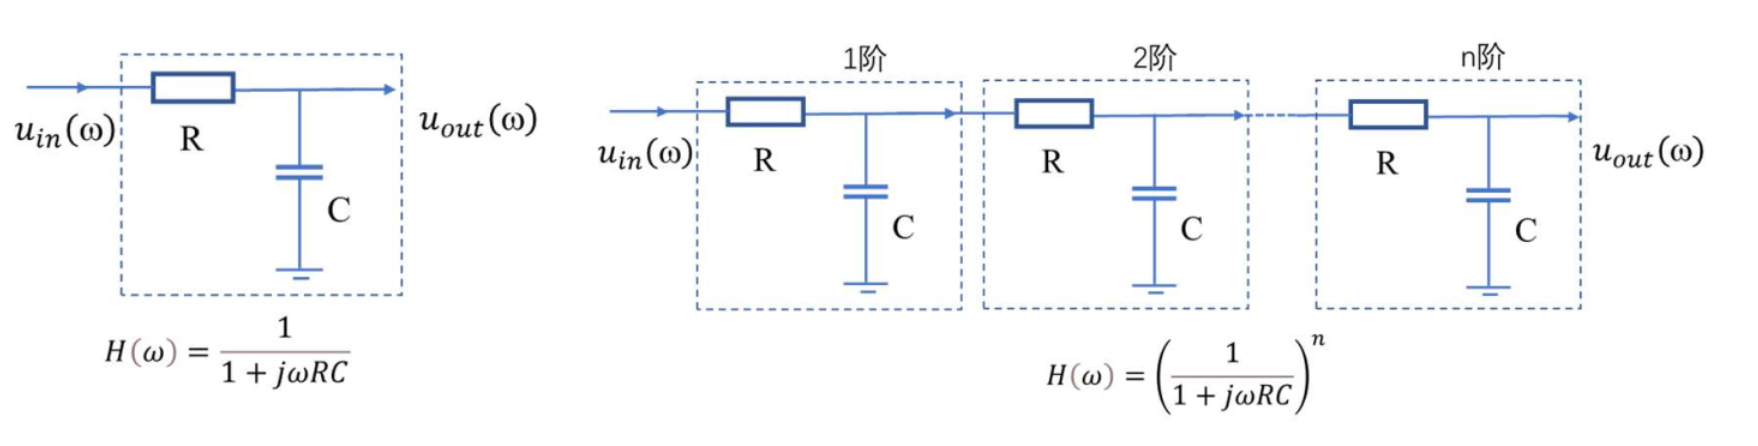
\includegraphics[width=1\linewidth]{原理1.png}
	\caption{多个RC低通滤波器级联}
	\label{}
\end{figure}
\subsubsection{锁相放大法提升信噪比}
锁相放大法(Lock-in Amplification)是一种高灵敏度信号检测技术,广泛应用于物理、电子工程和其他科学领域,尤其在测量微弱信号时表现突出。其基本原理和工作步骤如下:

锁相放大法通过调制和解调的方式,将待测信号从噪声中提取出来。其核心在于使用相敏检测技术,这使得该方法能够有效地隔离信号与噪声。

工作步骤
\begin{enumerate}
	\item 信号调制:将待测的微弱信号 \( s(t) \) 与一个高频正弦载波 \( \cos(𝜔ₘ t) \) 相乘。这一过程将信号频谱迁移至调制频率 \( 𝜔ₘ \) 附近。这种频谱迁移有助于避免低频噪声(如1/f噪声)的干扰。
	\item 相敏检波:使用相敏检波器(PSD)对调制后的信号进行解调。PSD能够通过参考信号(与调制信号同频且相位相同)提取目标信号。由于噪声的相位通常不同于信号,因此噪声的影响被显著降低。
	\item 低通滤波:将解调后的信号通过一个窄带低通滤波器(LPF),进一步去除高频噪声和不必要的频率成分。低通滤波器的带宽设计得非常窄,使得只有调制频率附近的信号能通过,从而提高信噪比。
\end{enumerate}
\subsection{锁相放大器工作原理}
锁相放大器的基本结构如图 2(b) 和 (c) 所示的虚线框内, 其中信号通道、参考通道为锁相放大器的输入通道,相敏检测器(PSD)和低通滤波器(LPF)等。

\begin{figure}[{H}]
	\centering
	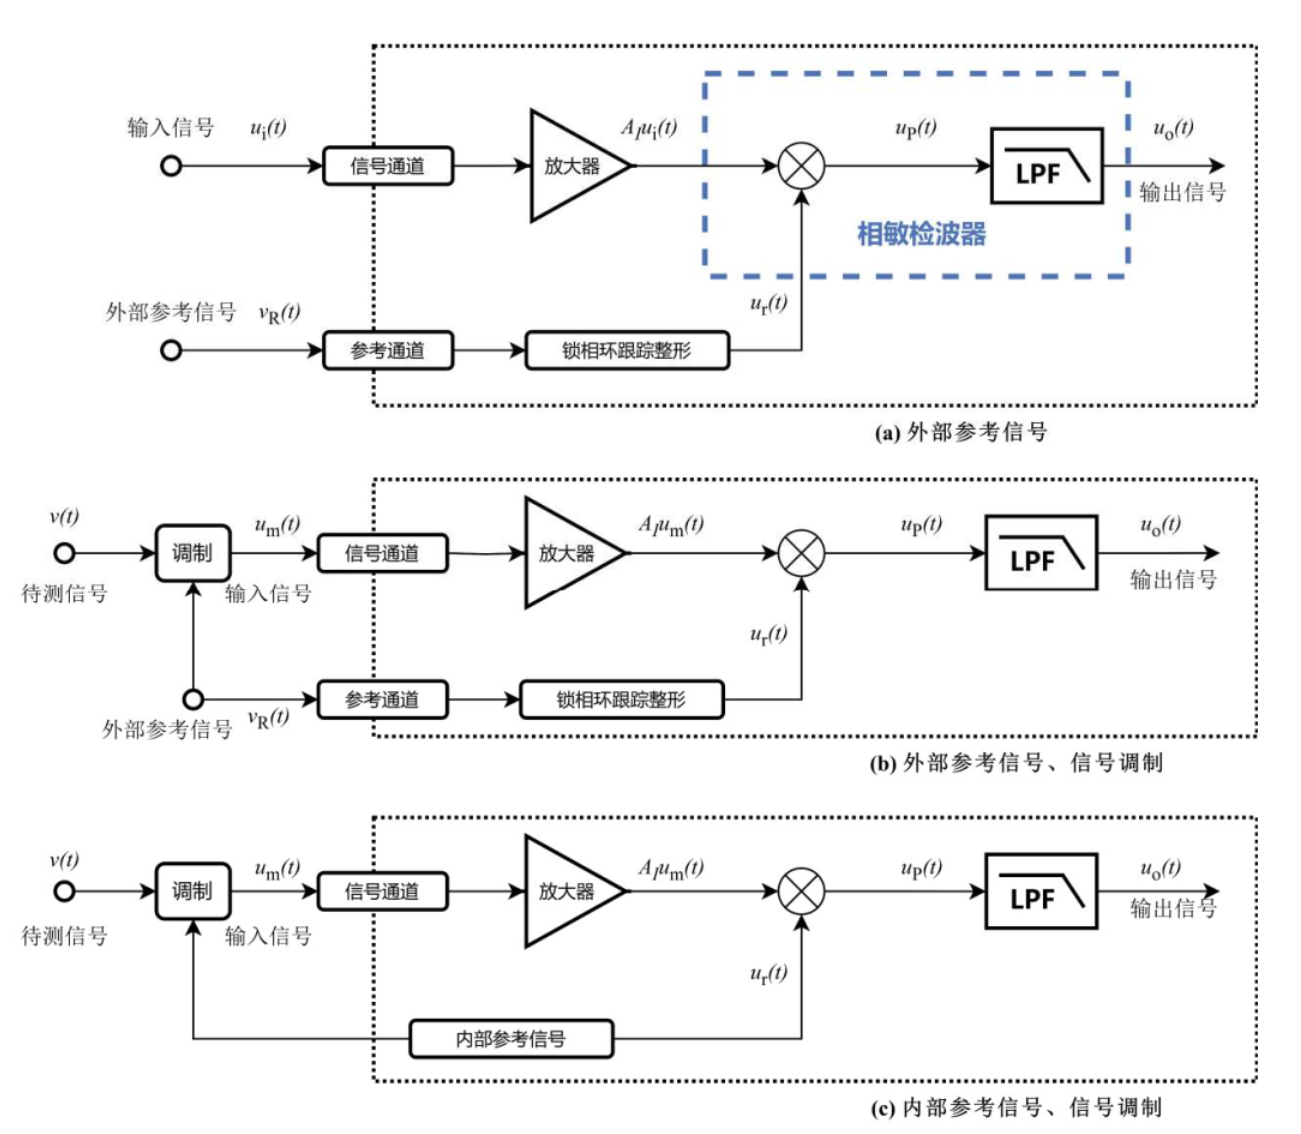
\includegraphics[width=0.8\linewidth]{原理2.png}
	\caption{锁相放大器的工作原理}
	\label{}
\end{figure}


对于三角函数信号 \(u_i(t) = u_0 \sin (\omega_s t + \phi)\),可直接从信号通道输入(虚线框内的)锁相放大器,此时待测信号即为锁相放大器的输入信号。对于非三角函数信号或慢变信号(如直流信号),它在输入锁相放大器前,需要被与参考信号频率相同的正弦信号所调制。原则上,参考信号既可以是外部输入信号 \(v_R(t)\) 经整定后得到的正弦信号,也可以是锁相放大器内部自带参考信号源提供的正弦信号。实际操作上,因外部输入的参考信号不可避免地受到干扰和变形,要求锁相环对外部信号有很强的整定能力。为改善信号处理效果,现在的锁相放大器内部都有自带的参考信号,且使用内部参考信号的效果优于外部参考信号。

三角函数信号可视为被调制的直流信号。一般情况下,下面以非三角函数信号为待测信号,使用数学方式阐述锁相放大器的工作原理。对于噪声,它可以叠加在调制前的信号中,也可以叠加在调制后的信号中;锁相放大器信号输入端不能区分这两种情况,因此,下面推导中只考虑后者,即输入信号为三角函数,输入噪声为 \(n(t)\)。

调制前信号包含待测信号和噪声,有:
\begin{equation}
    v(t) = s(t) + n(t)
\end{equation}

经 \(\sin (\omega_m t + \theta)\) 信号调制后:
\begin{equation}
    u_m(t) = x(t) \sin (\omega_m t + \theta) = s(t) \sin (\omega_m t + \theta) + n(t)
\end{equation}

其中, \(n(t) = v_N(t) \sin (\omega_m t + \theta)\)。

\begin{enumerate}
    \item 输入:式(8)给出了锁相放大器的输入信号 \(u_{\text{in}}(t)\)。
    \item 放大:输入信号仍然很弱,在经前置放大器后被放大 \(A_I\) 倍:
    \begin{equation}
        u_a(t) = A_I s(t) \sin (\omega_m t + \theta) + A_I n(t)
    \end{equation}
    此时,信号与噪声都被同时放大了。
    \item 解调:锁相放大器采用参考信号 \(u_r(t) = \sin (\omega_r t)\) 解调:
    \begin{equation}
        u_{px}(t) = u_r(t) u_s(t) = A_I [s(t) \sin (\omega_m t + \theta) \sin (\omega_r t) + n(t) \sin (\omega_r t)]
    \end{equation}
    \[
        = A_I \left\{s(2t) \left[\cos ((\omega_m - \omega_r) t + \theta) - \cos ((\omega_m + \omega_r) t + \theta)\right] + n(t) \sin (\omega_r t)\right\}
    \]

    对于调制信号是通过某种物理机制由参考信号触发或用参考信号本身情况,参考信号与调制信号频率相同 (\(\omega_m = \omega_r\)),相位差 \(\theta\) 确定;并经过理想的低通滤波器滤去高频分量,则滤波器输出信号为:
    \begin{equation}
        u_{ox}(t) = A_I \left[\frac{1}{2} s(t) \cos \theta + n_x(t)\right]
    \end{equation}
    式中,\(n_x(t)\) 为未被滤去的、与参考频率相同的“同频噪声”,一般情况下其幅值远小于信号,即对高信噪比情况:
    \begin{equation}
        u_{ox}(t) = s_{ox}(t) = \frac{1}{2} A_I s(t) \cos \theta
    \end{equation}
    锁相放大器输出信号 \(s(t)\) 有效值:
    \begin{equation}
        X = \frac{\sqrt{2} u_{ox}(t)}{A_I} = R \cos \theta
    \end{equation}

    为了获得完整的输入信号,需采用另一路频率相同、且与参考信号相位相差 \(\pi/2\) 的信号 \(u_{r1}(t) = \cos (\omega_r t)\) 作为解调信号, 则通过相敏检测后此路信号与另一路信号也相差 \(\pi/2\):
    \begin{equation}
        s_{py}(t) = \frac{1}{2} A_I s(t) \left[\sin ((\omega_m - \omega_r) t + \theta) + \sin ((\omega_m + \omega_r) t + \theta)\right]
    \end{equation}
    \begin{equation}
        s_{oy}(t) = \frac{1}{2} A_I s(t) \sin \theta
    \end{equation}
    \[
        Y = \frac{\sqrt{2} u_{oy}(t)}{A_I} = R \sin \theta
    \]
    \begin{equation}
        R = \sqrt{X^2 + Y^2}
    \end{equation}
    定义锁相放大器输入信号相对于解调信号(图 3 的参考信号)的相位差:
    \begin{equation}
        \theta = \tan^{-1} \frac{u_{oy}(t)}{u_{ox}(t)}
    \end{equation}
    这种可同时测量完整输入信号信息的锁相放大器称双相锁相放大器。
\begin{figure}[{H}]
	\centering
	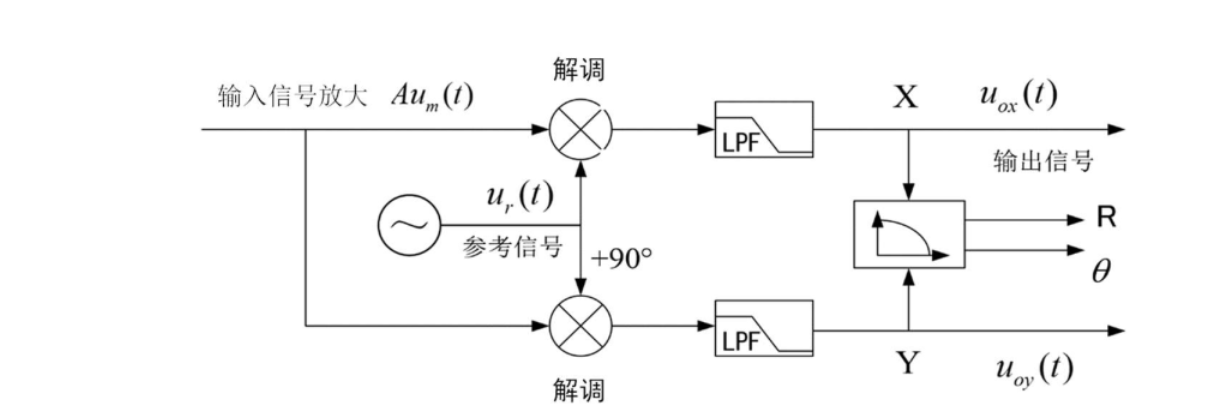
\includegraphics[width=0.8\linewidth]{原理3.png}
	\caption{双锁相放大器}
	\label{}
\end{figure}
    \item 然而,实际滤波器并不理想,且滤波器的性能与锁相放大器参数设置(选择)有关。要用好锁相放大器,就需要对滤波器的工作原理有更深入的了解。先讨论未被滤波(时间常数很小)时,从式(10)和式(14):
    \begin{equation}
        R(t) = s(t) |\sin (\omega_m t + \theta)|
    \end{equation}
    即信号项被 \(|\sin (\omega_m t + \theta)|\) 所调制,其频率是被调制信号频率 \(\omega_m\) 的 2 倍。对 \(|\sin (\omega_m t + \theta)|\) 做傅里叶变换,可得到该频谱,即 2\(\omega_m\) 频率下的幅值和直流分量(平均值)。在信噪比较高时,此式容易被观察到。
\end{enumerate}
\subsection{名称由来}

在许多应用场合中,锁相放大器的参考信号是由外部设备提供的,例如光学斩波器或信号发生器。这种工作模式称为“外部参考模式”(external reference mode)。在这种模式下,锁相放大器的参考通道会接收外部输入的参考信号,并对其进行放大和整形。参考信号通常是正弦波或近似正弦波的周期信号,可能由于噪声或失真而有所变形。为确保后续信号处理的准确性,锁相放大器首先会通过放大器和整形电路将该外部信号处理为一个更为标准、纯净的信号,去除掉噪声和畸变的影响。

在信号整形之后,锁相放大器会使用锁相环(Phase-Locked Loop,简称PLL)技术对外部输入的参考信号进行频率和相位的跟踪。这意味着锁相环会根据输入参考信号产生一个与其频率相同、且相位差锁定的正弦信号。这个锁相环生成的信号即是图 D1-7(b) 所示的 \( u_r(t) \)。这个新生成的参考信号相当于一个理想的版本,保留了外部参考信号的主要特性(如频率),但消除了由于干扰或噪声引起的畸变。这样,锁相放大器可以在保持参考信号准确性的同时,进行高精度的信号检测和分析。

“锁相”的概念在这里指的是:通过锁相环(PLL),锁定外部参考信号与内部生成的参考信号之间的相位关系,确保两者具有相同的频率和确定的相位差。相位差的锁定是锁相放大器实现相敏检测(phase-sensitive detection,PSD)的基础。相敏检测是锁相放大器的核心功能,它允许设备通过与参考信号进行比较,检测到与输入信号同步的部分,滤除掉不相关的噪声和干扰成分,从而提高信号测量的精度。

使用外部参考信号时,锁相放大器能够灵活地处理各种不同来源的周期性信号。这在实际应用中非常有用,尤其是当测量系统中使用的信号源(如光学斩波器或信号发生器)已经包含了周期性参考信号时。通过外部参考模式,锁相放大器能够自动与这些外部参考信号同步,不仅保持了与外部设备的协调性,还避免了因噪声或相位漂移导致的测量误差。

总体而言,锁相放大器的外部参考模式使得其在多种复杂环境下的应用成为可能。无论是光学实验、无线电频率测量,还是其他需要高灵敏度信号检测的领域,锁相放大器都可以通过精确锁定外部参考信号,实现高效的信号提取和测量。这也是锁相放大器在科研和工业测试中的广泛应用的关键所在。

	\subsection{原理部分思考题}
	
	% 思考题1
	\begin{question}
		市频 50Hz 干扰通常通过电源耦合,影响仪器的测量结果;对于 997Hz 的待测信号,
50Hz 干扰是噪声吗?对锁相放大器的测量会有影响吗?
	\end{question}
	50Hz 的市频干扰对于 997Hz 的待测信号确实是噪声,但为避开市电 50Hz 及其整数倍频率外部干扰,
待测信号选择了 997Hz,因此对于锁相放大器而言测量几乎不存在影响。
	% 思考题2
	\begin{question}
		如何用锁相放大器检测到待测的直流信号或慢变信号?
	\end{question}
	在锁相放大器的使用中,首先需要对待测信号 \(x(t)\) 的频谱进行迁移,即进行调制。其调制过程是将待测信号 \(x(t)\) 乘以频率为 \(\omega_0\) 的正弦载波。例如,待测信号可以表示为:
\[
x(t) = s(t) + n(t)
\]
经过信号 \(\sin(\omega_0 t + \theta)\) 调制后,变为:
\[
u(t) = x(t) \sin(\omega_0 t + \theta) = s(t) \sin(\omega_0 t + \theta) + n(t) \sin(\omega_0 t + \theta)
\]
从而将其频谱迁移到调制频率 \(\omega_0\) 附近。

接下来,对信号进行选频放大处理,并使用相敏检测器对信号进行解调,将其频移到直流的两侧。之后,通过窄带低通滤波器滤除噪声,得到高信噪比的放大信号。这样,锁相放大器就能够检测到待测直流信号或慢变信号。

	% 思考题3
	\begin{question}
		如用斩波器调制直流信号(如光强),被斩制后的信号仍
然包含有直流分量(即平均值不为零),但该直流分量随交流信号输入锁相放大器后
不会被锁相放大器检测,请从数学推导上说明。
	\end{question}
	被斩波器调制后的信号为:
\[
A(t) = u_m(t) + a = [s(t) + n(t)] \sin(\omega_0 t + \theta) + a
\]
其中 \(a\) 为直流分量。经过锁相放大器后得到:
\[
B(t) = A_l [s(t) + n(t)] \sin(\omega_0 t + \theta) + A_l a
\]
此处 \(A_l\) 为锁相放大器的放大倍数,之后再经过参考信号 \(u_r(t) = \sin(\omega_0 t)\) 解调得到信号:
\[
B(t) = \frac{A_l}{2} [s(t) + n(t)] (\cos \theta - \cos(2 \omega_0 t + \theta)) + A_l a \sin(\omega_0 t)
\]
这里 \(\omega_0\) 为高频频率,因此经过低通滤波后,低频分量 \(\frac{A_l}{2} [s(t) + n(t)] \cos \theta\) 得到保留,而高频分量 \(\frac{A_l}{2} [s(t) + n(t)] \cos(2 \omega_0 t + \theta)\) 以及 \(A_l a \sin(\omega_0 t)\) 将被滤过。由此可见,直流分量会被过滤而不会被放大。

此外,若 \(a\) 为慢变信号,不妨设 \(a = \sin(\omega_1 t)\),则其经过解调后变为:
\[
A_l \sin(\omega_1 t) \sin(\omega_0 t) = \frac{A_l}{2} [\cos(\omega_1 t - \omega_0 t) - \cos(\omega_1 t + \omega_0 t)]
\]
此时两个信号也都是高频信号(\(\omega_1\) 的值非常小),经过低通滤波器后均会被滤去,因此直流分量随交流信号输入锁相放大器后不会被锁相放大器检测到。


	\begin{question}
		相位以及相位差的含义是什么?锁相放大器输出的是待测信号的相位还是待测信号
与参考信号之间的相位差?
	\end{question}
	相位是交流信号中的相角,例如信号 \(x(t) = A e^{i(\omega t + \phi)}\) 的相位为 \(\phi\)。相位差是指两个交流信号的相位之差。设两个交流信号分别为:
	\[
	x_1(t) = A e^{i(\omega t + \phi_1)}, \quad x_2(t) = A e^{i(\omega t + \phi_2)}
	\]
	则两个交流信号的相位差为:
	\[
	\phi_1 - \phi_2
	\]
	锁相放大器输出的 \(\theta\) 是待测信号与参考信号之间的相位差。

	\begin{question}
		(选)以上仅讨论了滤波器的幅频特性,那么其相频特性又会是怎样呢?在时域的时
间响应特性又是怎样呢?感兴趣的同学可以自己推导。进一步,该相频特性会影响到
相位角$\theta$的测量吗?
	\end{question}
	锁相放大器的相频特性为:
	\[
	\Delta \theta = \frac{L}{v} \times 2\pi f
	\]

	该特性会影响相位角 \(\theta\) 的测量。

	% ---
	
	
	
	% 实验记录	
	\clearpage
	\section{D1 锁相放大器与弱信号测量(1) \quad\heiti 预习报告}
	% ---
	
	% 实验目的
	\subsection{实验目的}
	\begin{enumerate}
		\item 了解锁相放大器工作原理和特点,理解信号、噪声、信噪比等概念。
		\item 掌握锁相放大器基本参数含义及锁相放大器的基本操作,学会合理选择或调节参数(频
		率、相位、灵敏度、时间常数、陡降);复习示波器的使用;
		\item 掌握用锁相放大器检测弱信号方法,通过与示波器比较其检测能力了解其技术优势。
	\end{enumerate}
	% ---
	\subsection{实验要求}
	\begin{enumerate}
		\item 把锁相放大器作为测量工具,理解其工作原理:
		\begin{enumerate}
			\item 基本概念:信号、噪声、信噪比;时域谱、频域谱;
			\item 锁相放大器工作原理:信号的调制、解调(相敏检波)、滤波的数学表述;
		\end{enumerate}
		
		\item 学习合理地设置锁相放大器参数,为后面实验应用锁相放大器及时、准确、精密地
		获得待测微弱信号的之间获得合理的平衡。锁相放大器参数(频率、相位、灵敏
		度、时间常数、陡降)及其对锁相放大器测量的影响;
	
		\item 锁相放大器操作:参数设置,用示波器观察锁相放大器通道输出结果,或用
		DISPLAY 显示输出结果;
		
		\item 在实验报告中用实验结果回答问题。
		
		\item (选)参数设置和操作:浮地,差分(A-B)输入,外部输入参考信号(TTL 参考
		信号),扫频。
		
	\end{enumerate}
	% 仪器用具
	\subsection{仪器用具}
	\begin{center}
		\begin{tabular}{cm{4cm}cm{6cm}c}
				\hline
				编号 & 仪器用具名称 & 数量 & 主要参数(型号,规格等)  \\
				\hline
				1 & 锁相放大器 & 1 & OE1022(系列)   \\
				2 & 配套教学实验箱 & 1 &    \\
				3 & 示波器 & 1 & RIGOL DS2202A   \\
				4 & 信号发生器 & 1 & RIGOL DG4162  \\
				5 & BNC-BNC 信号线 & 若干 &    \\
				\hline
		\end{tabular}
		\end{center}
		

	
	
	
	% 实验前思考题
	\subsection{预习思考题题}
	
	% 思考题1
	\begin{question}
		噪声有哪些类型?一般测量对象本身的噪声是哪来的?它有什么特征?
	\end{question}
	噪声可分为来自外界的环境的有规律的声源(如市电噪声)以及来自被测量对象本身的噪声(如无规
的热噪声)。
对于一项实验,一般测量对象本身的噪声,最典型的比如无规的热噪声,既可来自于实验对象本身,也
可来自于测量系统,包括传感器和测量仪器。
	% 思考题2
	\begin{question}
		是否可以用 RIGOL DG4162 信号发生器产生白噪声取代教学实验箱产生的白噪声?如
何将它与信号混合?
	\end{question}
	可以用 RIGOL DG4162 信号发生器产生白噪声取代教学实验箱产生的白噪声。
按 Utility -> CH1 设置 -> 噪声叠加,用户可以打开或关闭噪声叠加功能。默认为“关闭”。选择“打
开”时,可以使用数字键盘或方向键和旋钮设置噪声比例。可设置范围为 0\% 至 50\%,默认值为 10.0\%。
当 Mod、 Sweep 或 Burst 开启时,噪声叠加菜单置灰禁用。
本实验中并未进行此操作,只是通过查阅 RIGOL DG4162 用户手册得知上述操作步骤。

	
	
	
	% 实验记录	
	\clearpage
	% 顶栏
	\begin{table}
		\renewcommand\arraystretch{1.7}
		\centering
		\begin{tabularx}{\textwidth}{|X|X|X|X|}
			\hline
			专业: & 物理学 & 年级: & 2022级 \\
			\hline
			姓名: &黄罗琳、 & 学号: & 22344001\\
			\hline
			室温: & 26℃ & 实验地点: & A101 \\
			\hline
			学生签名:& 
\includegraphics[width=1cm]{签字.jpg}  & 评分: &\\
			\hline
			实验时间:& 2024/9/20 & 教师签名:&\\
			\hline
		\end{tabularx}
	\end{table}
	% ---
	
	% 小标题
	\section{ D1 锁相放大器与弱信号测量(1)\quad\heiti 实验记录}
	% ---
	
	% 实验过程记录
	\subsection{用示波器观察内部信号输出(与参考信号同频同相)}
	OE1022 的内部振荡器 SINE OUT 相当于函数发生器,输出正弦信号。通过它产生一个幅
值为 80mVrms、频率约为 1kHz 的正弦波,并用示波器观察和记录波形及信号参数。

\begin{question}
		问题一:示波器是否显示出正弦波?其测量的信号参数值是否与锁相放大器的信号设置值
一致?
\end{question}


\begin{figure}[H]
    \begin{minipage}[b]{0.45\linewidth}
      \centering
      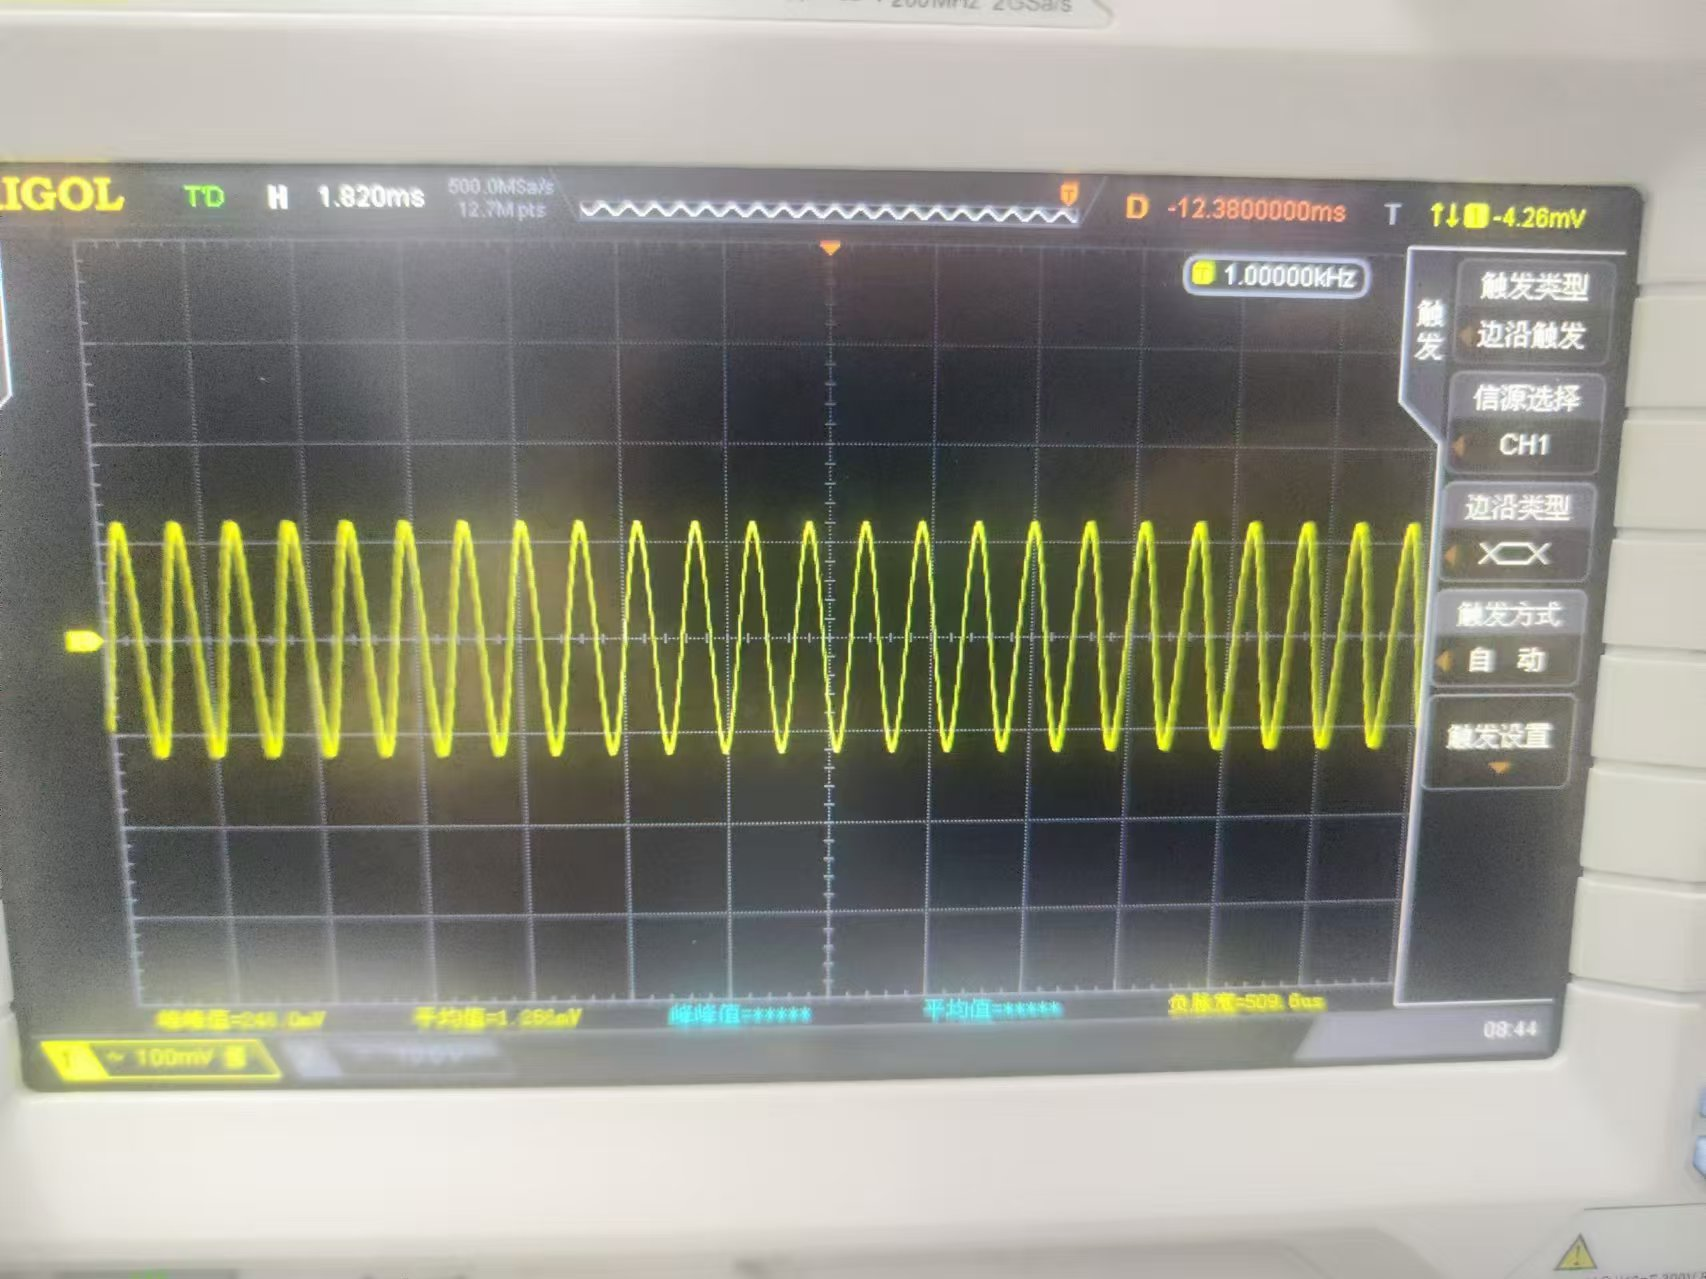
\includegraphics[width=\linewidth]{11.jpg} % 确保文件路径正确
      \caption{内部信号输出(1)}
    \end{minipage}
    \hfill
    \begin{minipage}[b]{0.45\linewidth}
      \centering
      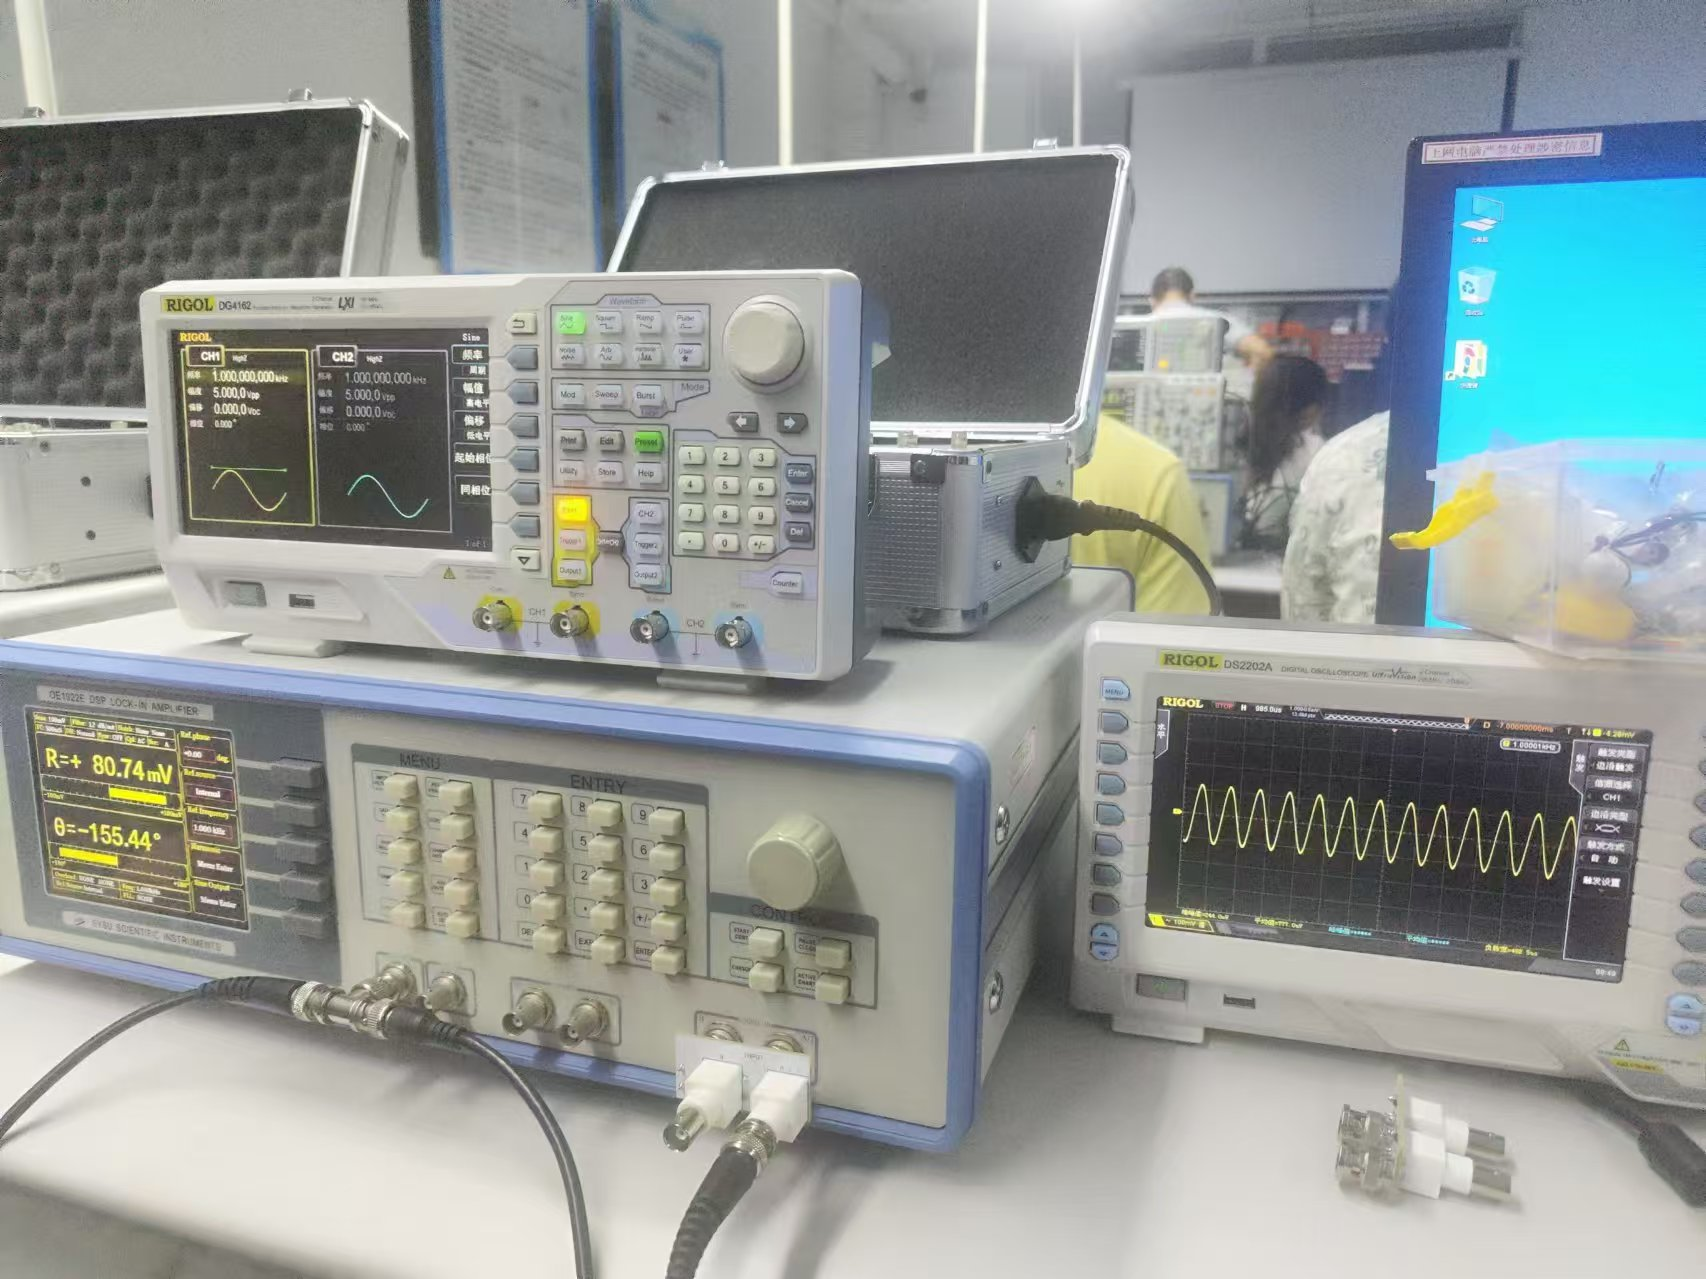
\includegraphics[width=\linewidth]{12.jpg} % 确保文件路径正确
      \caption{内部信号输出(2)}
    \end{minipage}
\end{figure}

如图所示,示波器输出的是正弦波。利用示波器测量其频率为 1kHz,与锁相放大器的信号设置参数一致;测得信号有效值为 84.85mVrms,与设定值相差 6.06\%。
\subsection{测量信号 $R$、$\theta$、$X$ 以及 $Y$ 值,并验证它们之间的关系
)}
\begin{enumerate}
    \item 用一条 BNC-BNC 信号线连接 OE1022 前面板 SINE OUT 输出接口和 SIGNAL IN 的 A/I 接口后,观察主界面中监测栏的 Overload 是否提示溢出:若前级输入溢出,则显示 Overload: INPUT NONE;若放大溢出,则显示 Overload: NONE GAIN;若同时溢出,则显示 Overload: INPUT GAIN。
    
    \item 若有前级溢出时应立即减小数字信号发生器输出幅值,若有放大溢出应立即调节量程灵敏度(sensitivity)值(OE1022 输入端峰值高于 1.7V 或谷值低于 -1.7V 时发生前级溢出,且默认量程灵敏度值为 100mV,因此本例中数字信号发生器输出幅值为 80mVrms 的正弦波时不会发生溢出,但是测量其他信号时要注意溢出情况)。
    
    \item 调节量程灵敏度值。按下前面板 GAIN/TC 按键进入子菜单。
    
    \item 按下软键 1 以选中 Sensitivity 功能,选中区域会有高亮显示,通过旋转旋钮调节 Sensitivity 值,使测量信号值尽量满偏而又不超量程。至此,我们即简单测出了从内置函数信号发生器输出的正弦波幅值大小以及相位。
\end{enumerate}
\begin{question}
	请比较示波器的读数和锁相放大器的$R$值,以理解$R$值的确切含义。
\end{question}
\begin{figure}[htbp]
    \centering
    \begin{minipage}{0.45\textwidth}
        \centering
        \includegraphics[width=\linewidth]{2.2.jpg}
        \caption{监测栏显示效果图}
        \label{fig:monitoring_display}
    \end{minipage}
    \hfill
    \begin{minipage}{0.45\textwidth}
        \centering
        \includegraphics[width=\linewidth]{2.1.jpg}
        \caption{直角坐标系中显示 $\theta$ 值随时间变化的效果图}
        \label{fig:theta_time_variation}
    \end{minipage}
\end{figure}

锁相放大器的输出值为 \( R = +80.74 \, \text{mV} \),而示波器所测得的有效值为 \( 84.85 \, \text{mV} \),这表明两者之间的数值基本一致,说明锁相放大器的输出信号与示波器的读数具有良好的相符性。这一测量值 \( R \) 代表的是锁相放大器输出信号经过调制、放大和解调后的有效值,其确切含义为电压方均根 \( V_{\text{rms}} \),即表示该交流信号的有效值。

有效值是交流信号的重要特性,它能够反映信号在一定时间内所提供的功率,与直流信号相同的功率值。在该实验中,通过锁相放大器处理的信号不仅被调制和放大,还经过了有效的解调,确保最终输出信号的准确性。这种处理过程使得测量结果更为可靠,为后续的信号分析和应用提供了基础。
\begin{question}
	测量数据反映出$R$、$X$、$Y$及$\theta$的之间是什么关系?是否与式(D1- 21)、式(D1- 24)和(D1- 25)符合?
\end{question}
根据测量结果,我们得到 \( R = +80.74 \, \text{mV} \),\( \theta = -155.44^\circ \),\( X = -73.44 \, \text{mV} \),以及 \( Y = 33.55 \, \text{mV} \)。


\[
R \cos \theta = 80.74 \, \text{mV} \times \cos(-155.44^\circ) \approx -73.44 \, \text{mV} \approx X
\]


\[
R \sin \theta = 80.74 \, \text{mV} \times \sin(-155.44^\circ) \approx -33.55 \, \text{mV} \approx Y
\]

因此,得出验证结果:
\[
X = R \cos \theta \quad Y = R \sin \theta
\]

这些计算结果表明 \( X \) 和 \( Y \) 确实与 \( R \) 和 \( \theta \) 的关系相一致,验证了它们之间的数学关系。

\begin{question}
	你使用的 OE1022 是双锁相放大器吗?为什么?
\end{question}
是单锁相放大器。

单锁相放大器的原理图如图所示,调制解调过的信号经过低通滤波后的输出信号 \( u_o(t) \) 仅存在一个信号输出 \( u_x(t) \)。在这种情况下,输出信号的相位信息通过与参考信号的比较获得,通常只输出一个通道的有效值。因此,单锁相放大器在功能上简化了信号处理流程,适用于对相位和幅度进行单一测量的应用场合。

\subsection{相敏检波器工作原理——乘法器}

当低通滤波器工作在宽带宽下时,锁相放大器的输出即使反映乘法器的输出。我们通过比较该输出与式 (D1-27),加深对相敏检波器工作原理的认识。

以测量一个幅值约为 $50 \, \text{mVrms}$、频率约为 $1 \, \text{kHz}$ 的正弦波信号为例输入 OE1022 锁相放大器,将滤波器带宽调至最大(TC=$10 \, \mu s$、Slope=$6 \, \text{dB/oct}$),锁相放大器输出可等效于乘法器输出;将锁相放大器模拟输出(Fast channel out)连接到示波器的输入进行观察。注意信号是否超量程,调节信号幅值或量程灵敏度(sensitivity)使之在合适量程以内(本例中,量程灵敏度设置为 $100 \, \text{mV}$ 至 $1 \, \text{V}$ 之间)。

\begin{question}
	示波器上看到的波形是什么?$X$、$Y$ 是正弦波吗?其相位差为多少度?$X$、$Y$ 的平均值为零吗?平均值是否会随滤波器参数而改变?参照式 (D1-19) 和式 (D1-23) 进行讨论。

$R$ 值波形是否呈现全波整流的正弦信号,其频率为多少?与 $X$ 或 $Y$ 的频率存在什么关系?请对比式 (D1-27) 讨论此波形。

\end{question}
\begin{figure}[htbp]
    \centering
    \begin{minipage}{0.45\textwidth}
        \centering
        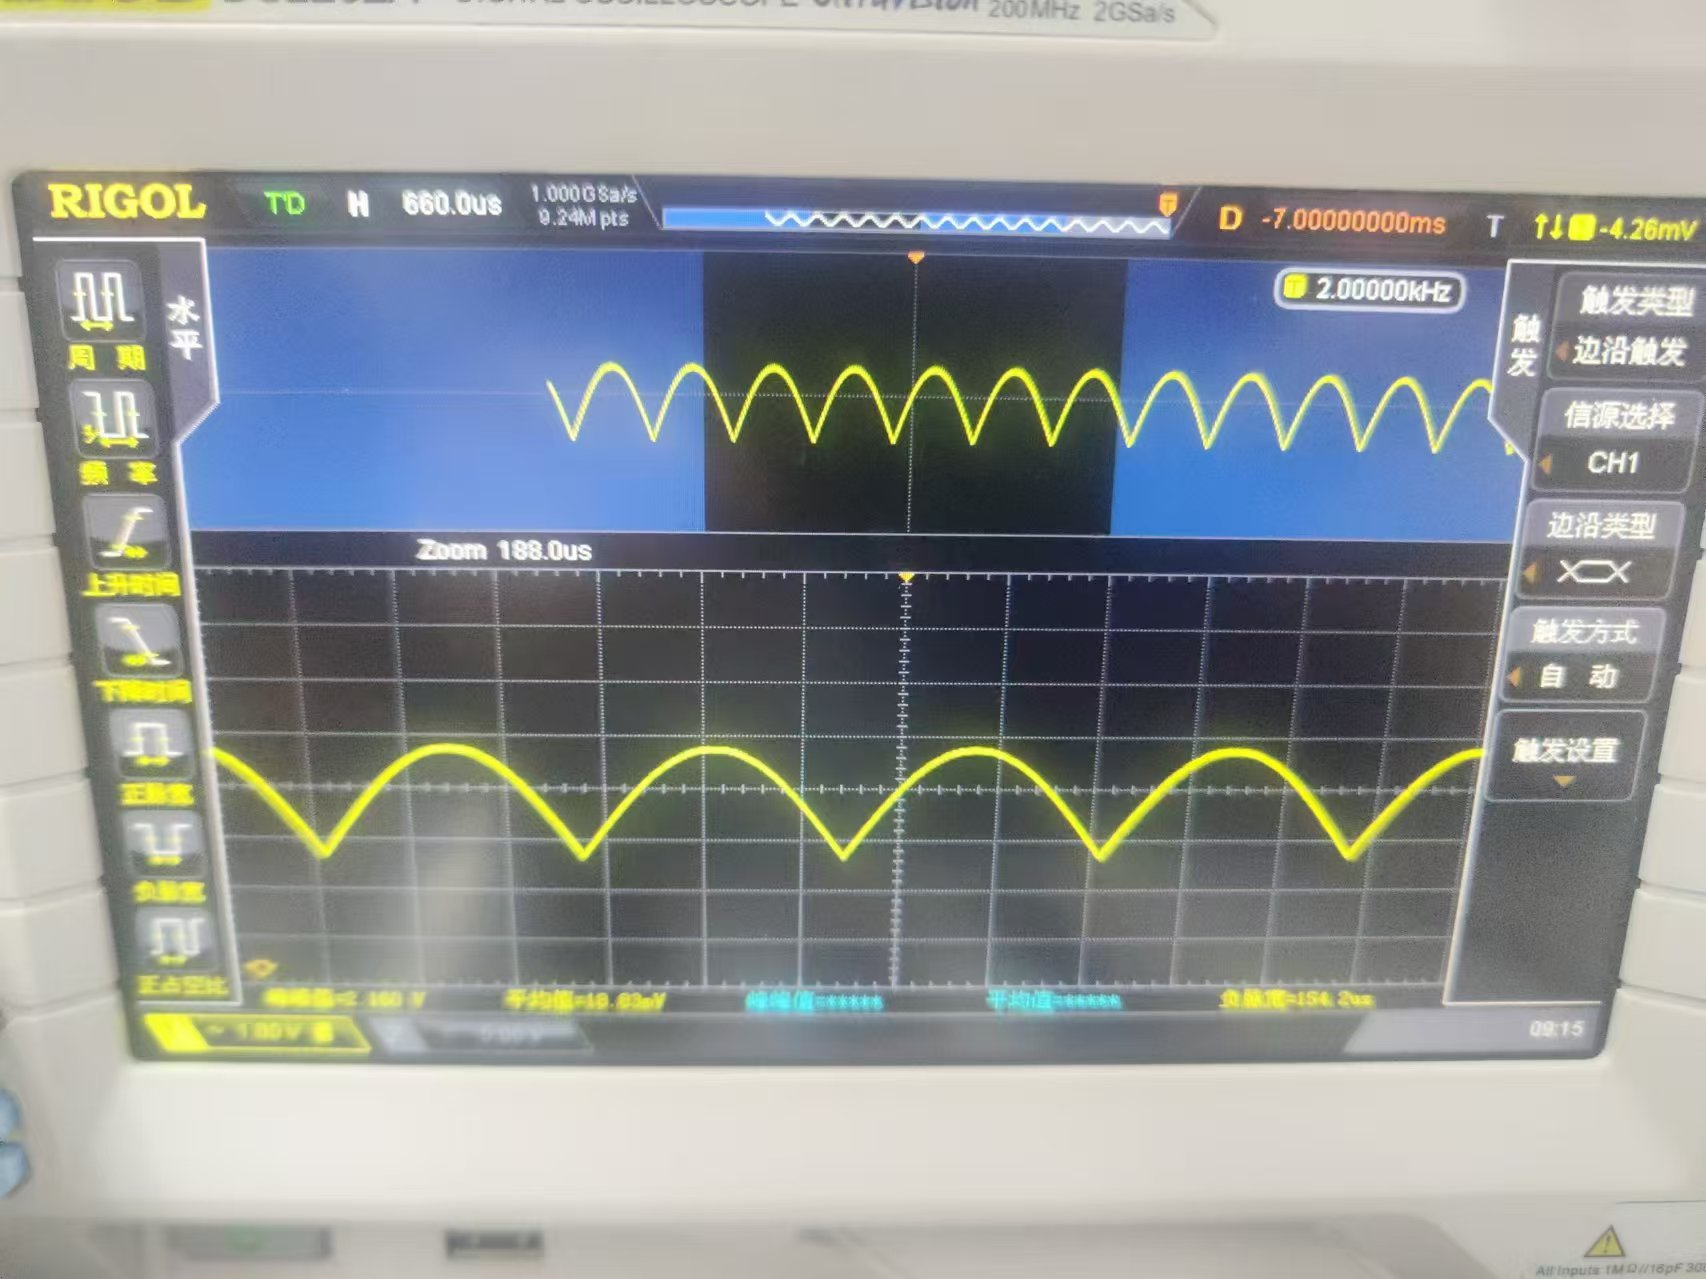
\includegraphics[width=\linewidth]{3.1.jpg}
        \caption{Fast 模式下 CH1 输出 R 信号波形}
        \label{fig:fast_mode_ch1_r_signal}
    \end{minipage}
    \hfill
    \begin{minipage}{0.45\textwidth}
        \centering
        \includegraphics[width=\linewidth]{3.2.jpg}
        \caption{接入示波器测量相位差}
        \label{fig:phase_difference_measurement}
    \end{minipage}
\end{figure}

	对于$XY$,均为正弦波,接入示波器进行测量,$XY$相位差为 $89.32^\circ$,接近 $90^\circ$,平均值不为零,会受到滤波器参数的影响,分析如下公式可知:
	$$u_{ox}(t)=A_I[\frac12s(t)\cos\theta+n_x(t)]$$
$$u_{oy}(t)=\frac12A_Is(t)\sin\theta$$

可能由于滤波器带宽调整导致信号频谱的变化,增益设置影响了信号的幅度,特别是在信号较弱或噪声较大的情况下从而影响了滤波效果,故平均值受滤波器参数影响。

对于$R$值波形,
$$R\left(t\right)=s(t)\left|\sin\left(\omega_mt+\theta\right)\right|$$

即信号项被$\left|\sin\left(\omega_mt+\theta\right)\right|$所调制,其频率是被调制信号频率$\omega_m$的 2 倍,所以从示波器波形看
到,R 值输出呈现全波整流的正弦信号,示波器显示频率 2kHz。
\subsection{相敏检波器工作原理——乘法器+低通滤波器}
\begin{question}
	当调大时间常数后,输出$R$是否越来越稳定?直流分量(信号平均值)是否有改变?
\end{question}
如图所示,保持滤波器陡降不变,通过增大时间常数,可以明显看出两信号越来越稳定,而信号的平均值产生了波动,但是观察最后哦两张图片,可以发现其是稳定的,这说明在完成滤波后,滤波效果较好时,信号的直流分量是稳定的。
\begin{figure}[htbp]
	\centering
	\subfloat[10 $\mu$s]{\label{10μs}
	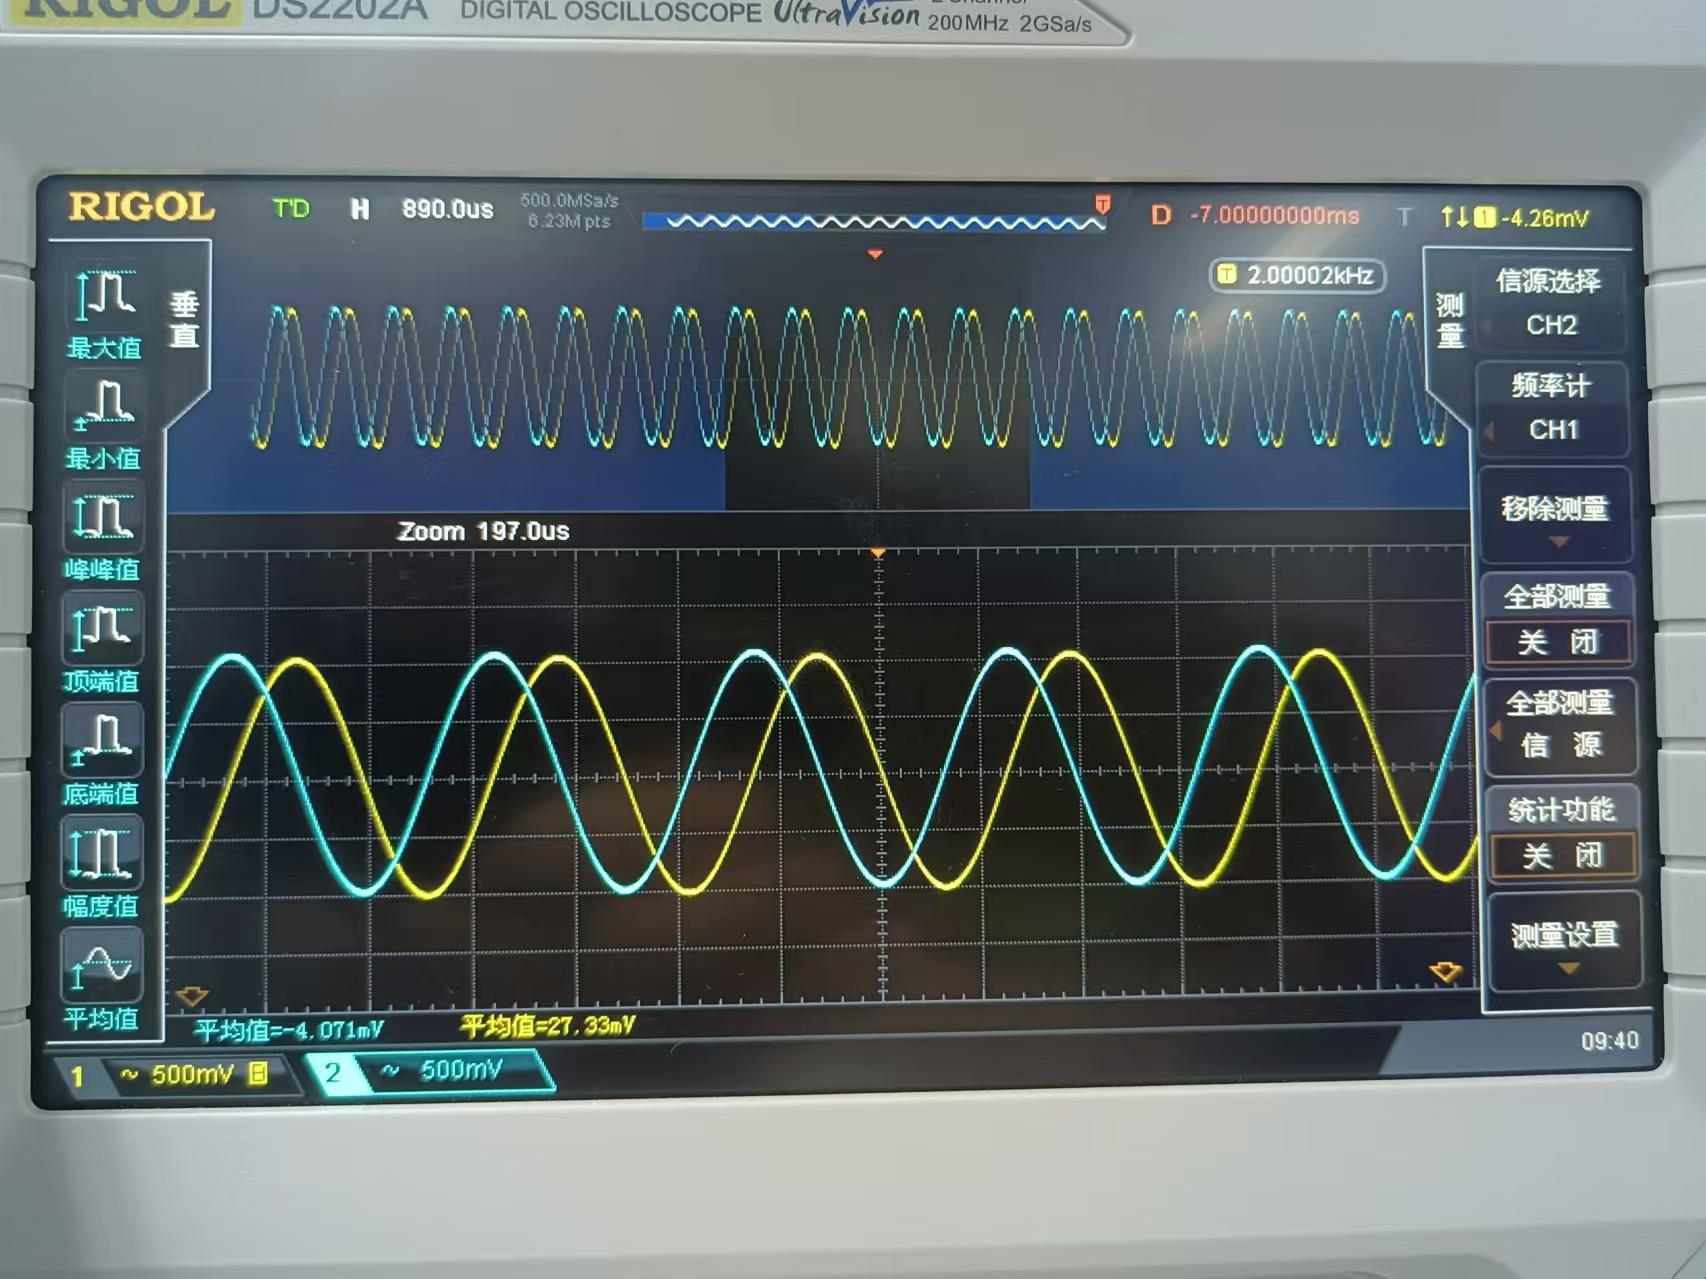
\includegraphics[width=0.28\linewidth]{10us.jpg}}
	\quad
	\subfloat[30 $\mu$s]{\label{30μs}
	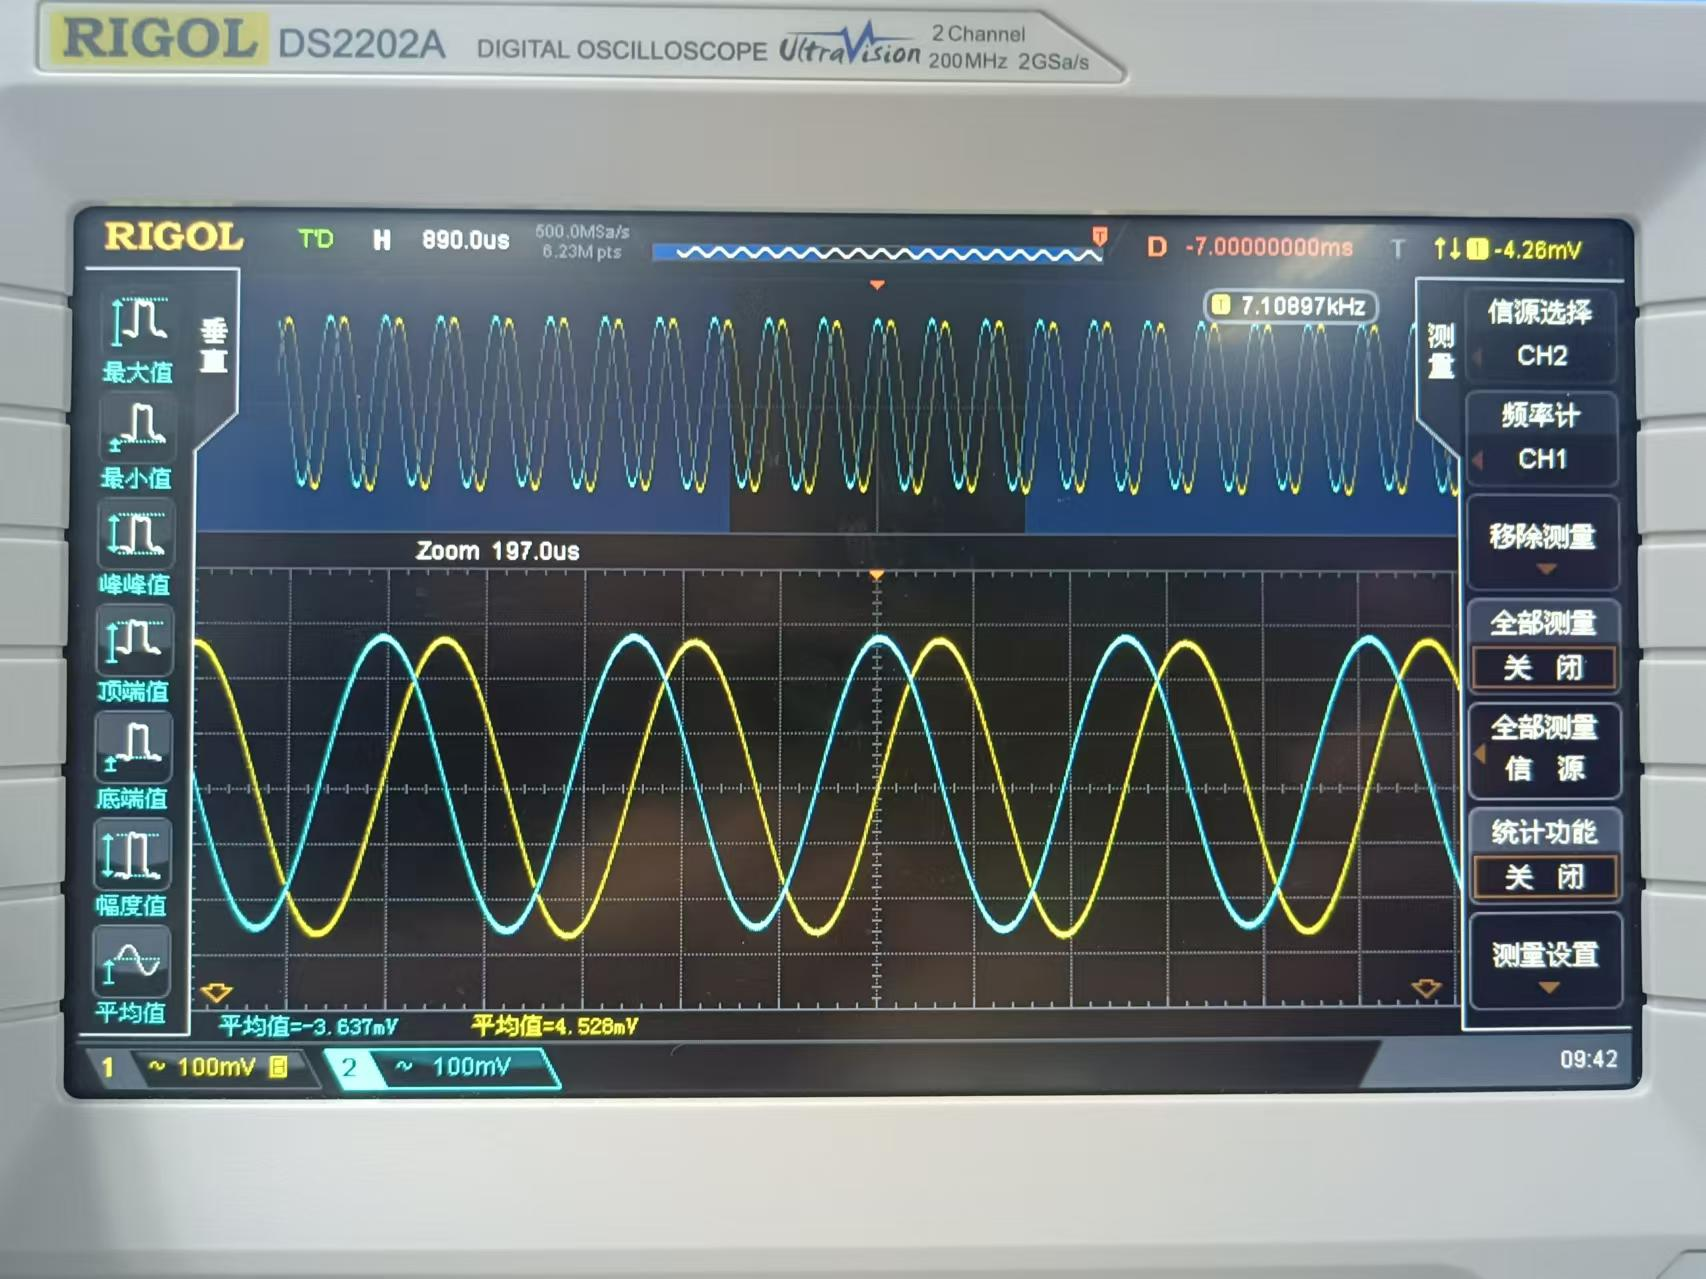
\includegraphics[width=0.28\linewidth]{30us.jpg}}
	\quad
	\subfloat[300 $\mu$s]{\label{300μs}
	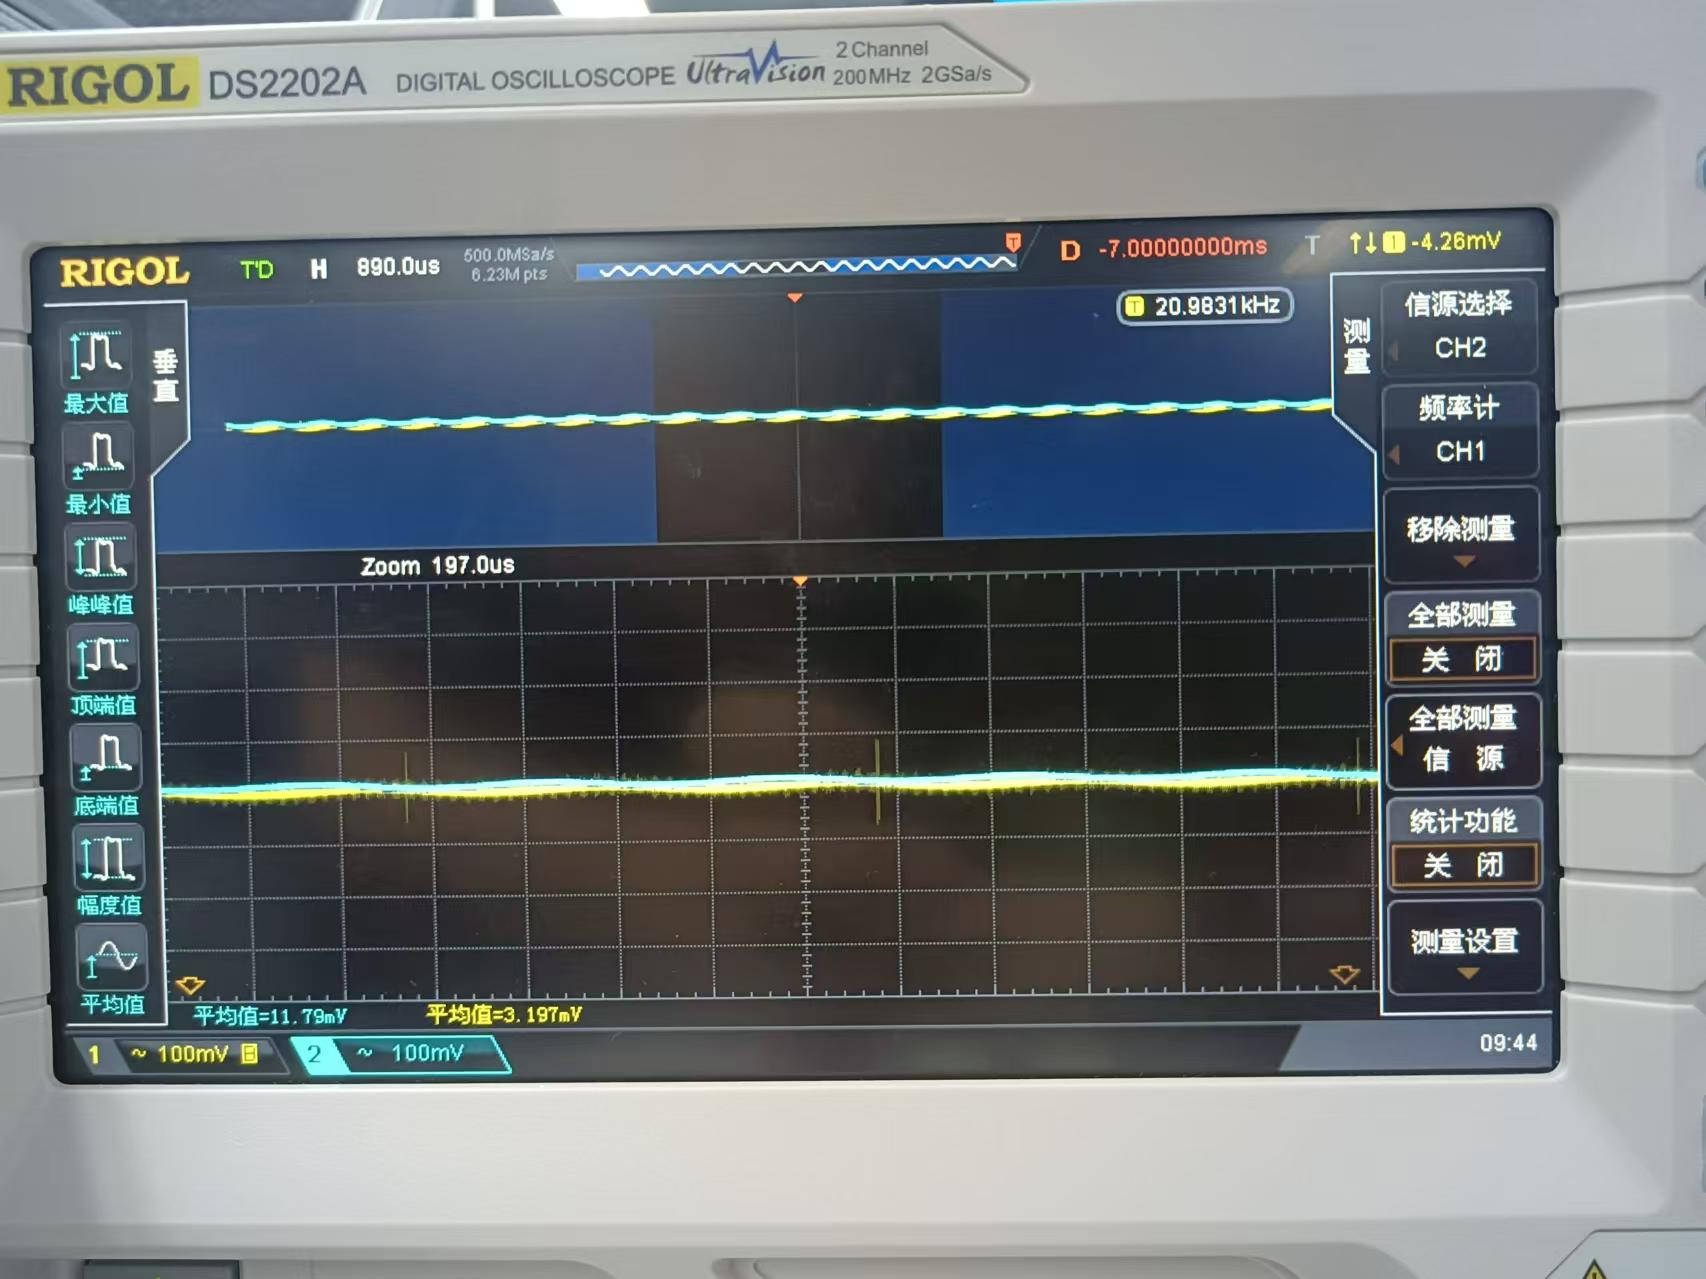
\includegraphics[width=0.28\linewidth]{300us.jpg}}\\

	\subfloat[1 ms]{\label{1ms}
	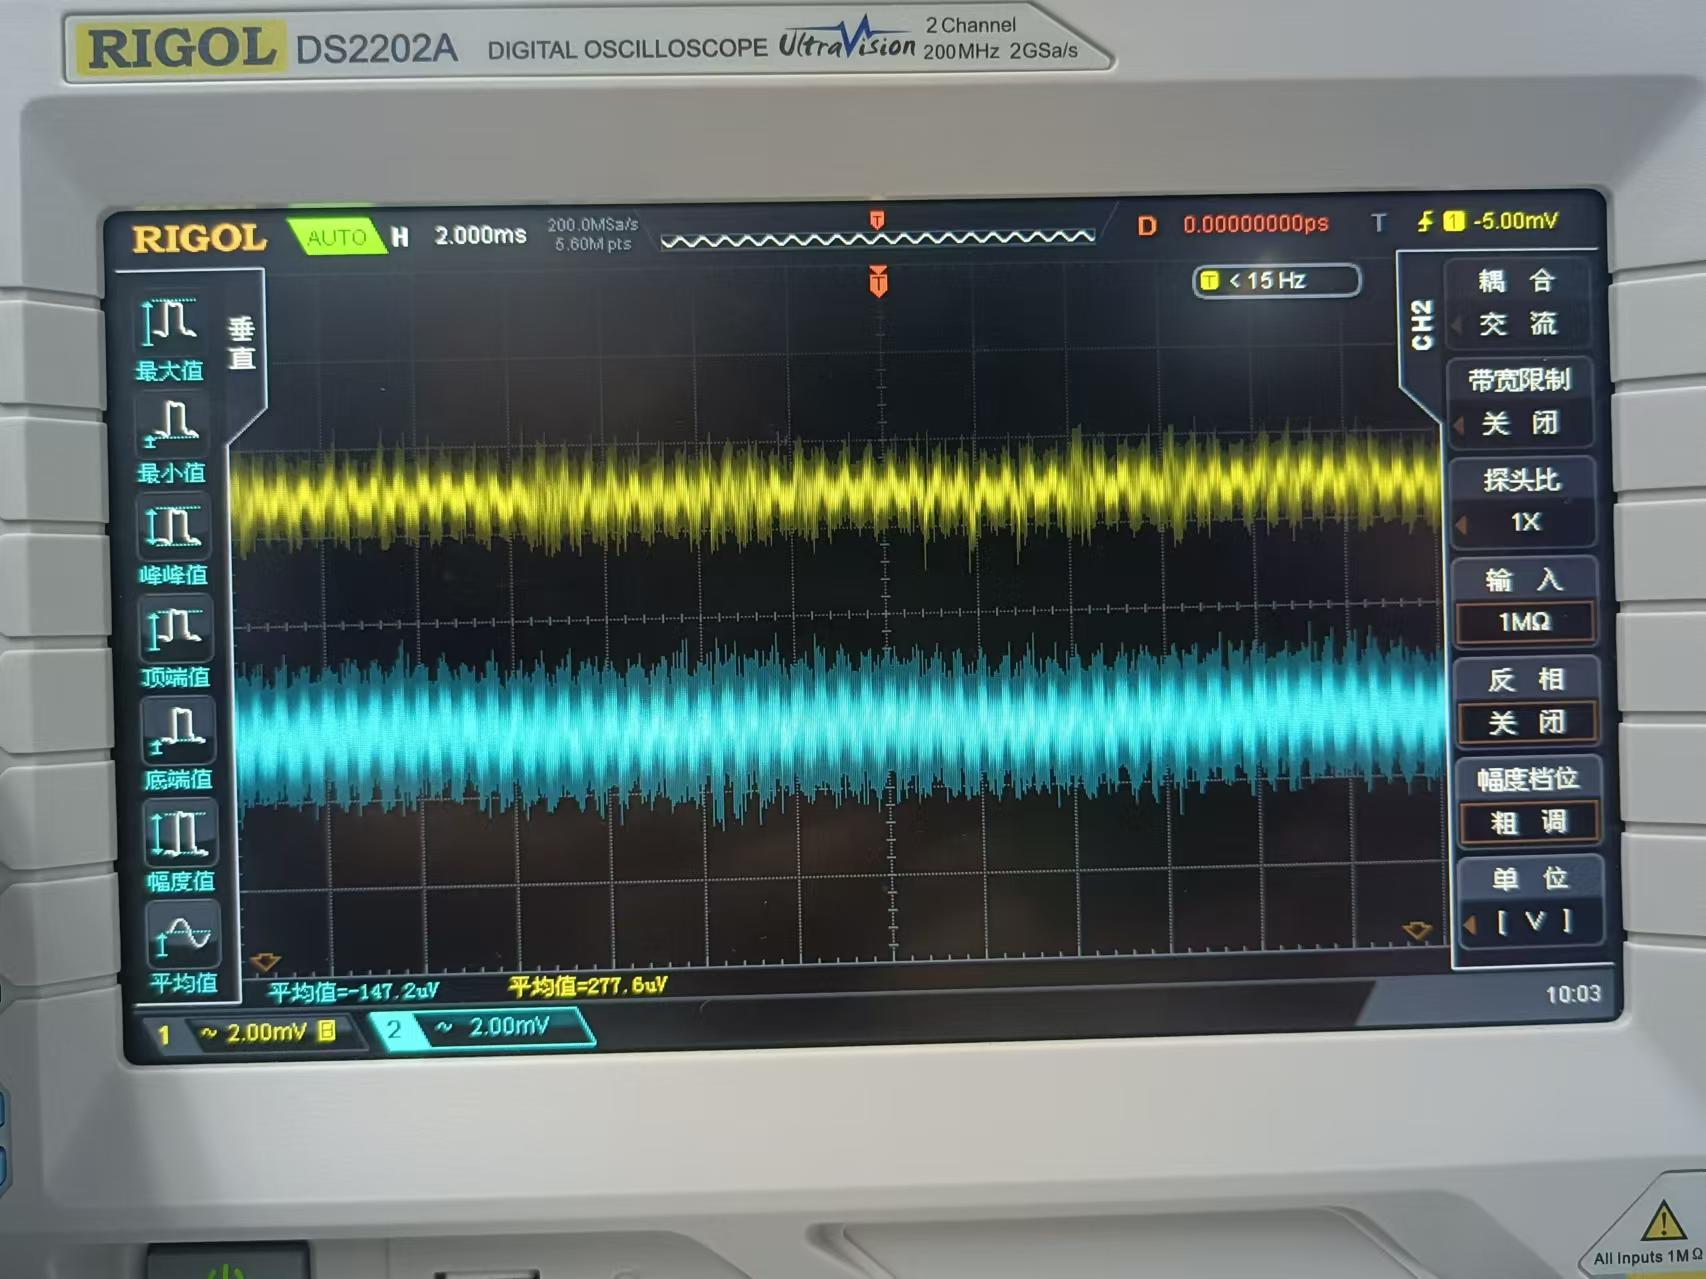
\includegraphics[width=0.28\linewidth]{1ms.jpg}}
	\quad
	\subfloat[3 ms]{\label{3ms}
	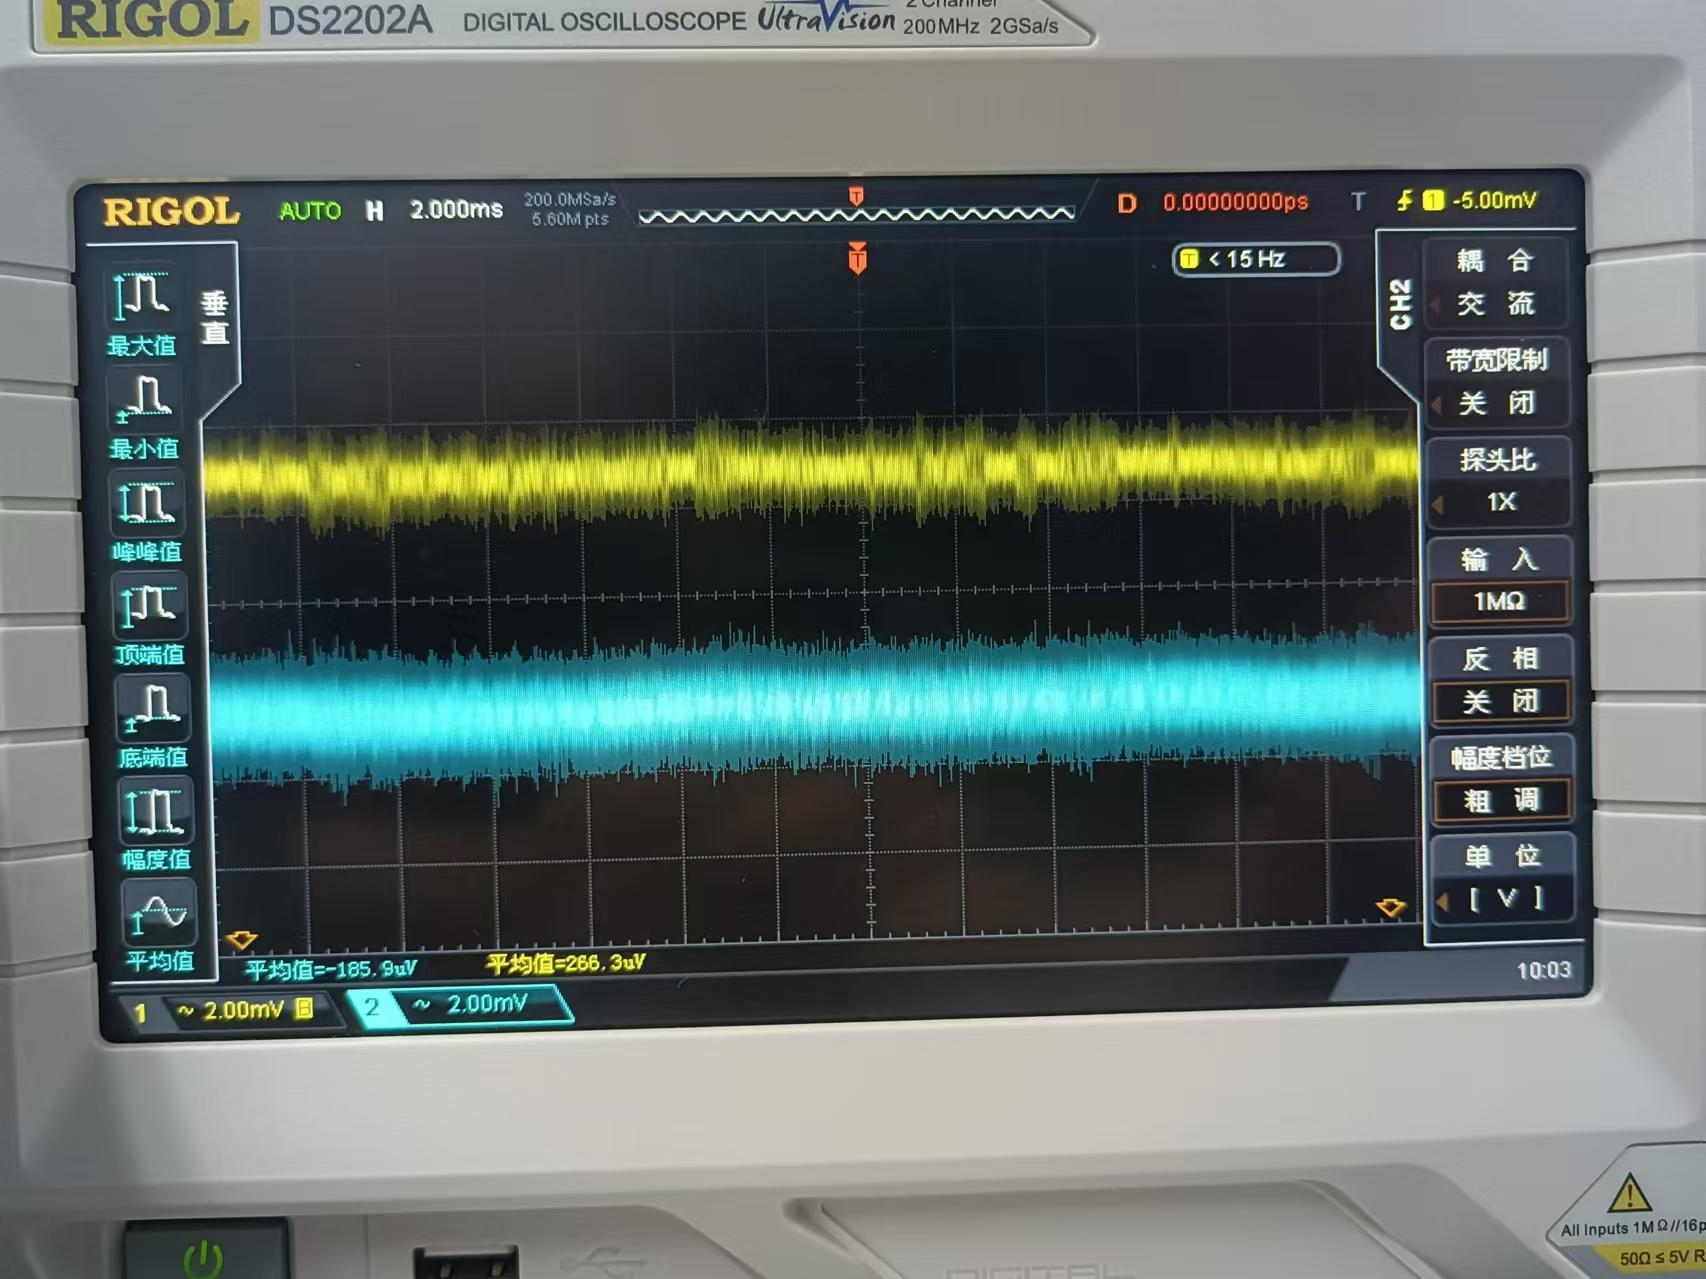
\includegraphics[width=0.28\linewidth]{3ms.jpg}}
	\quad
	\subfloat[10ms]{\label{10ms}
	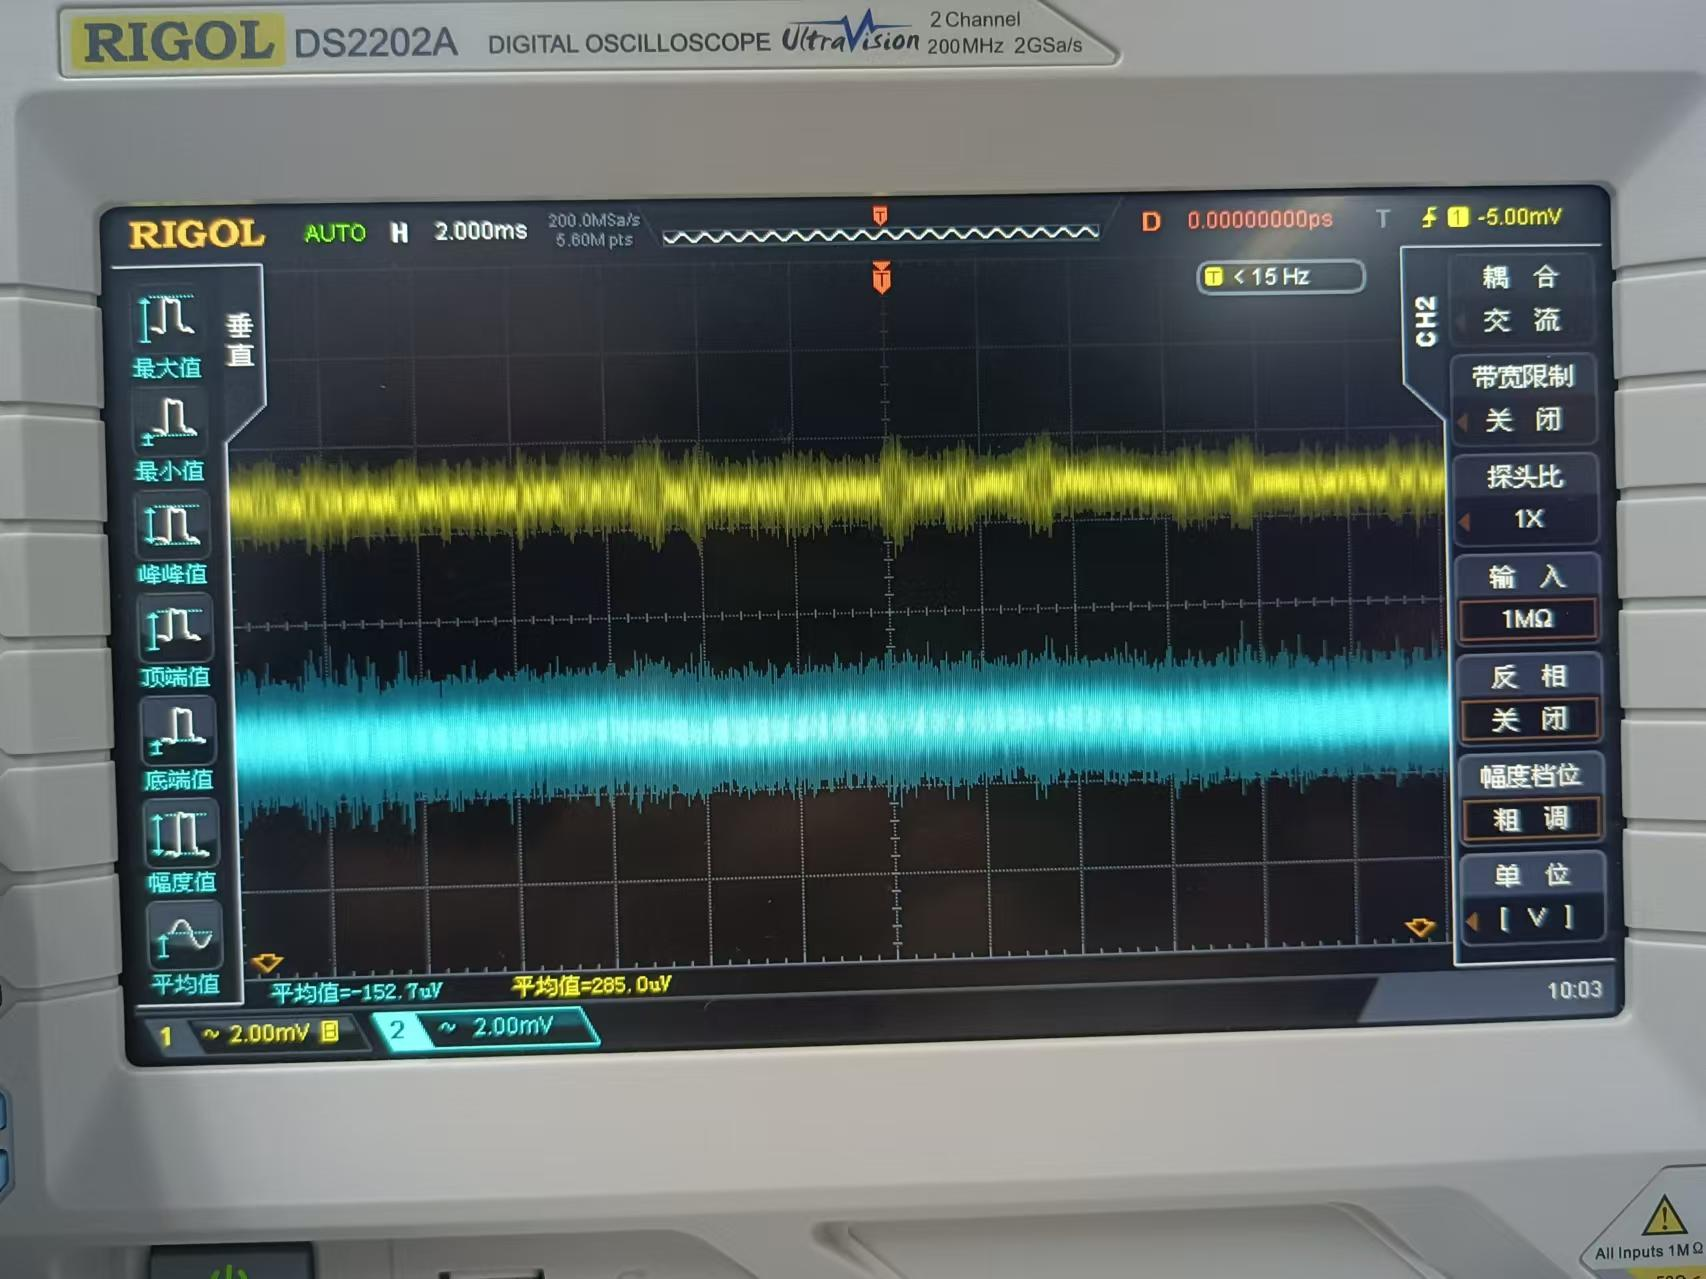
\includegraphics[width=0.32\linewidth]{10ms.jpg}}
	\caption{陡降 24 dB/oct 不变,增大时间常数,观察示波器波形}
	\label{fig:time_constant_effect}
\end{figure}
\begin{question}
	观察示波器波形,并给出在某一陡降值下,时间常数为多少个信号周期时,才能观
察到稳定的直流输出?提示:注意调节示波器$Y$轴量程以提高测量振幅变化的精度。
\end{question}
根据理论公式,时间常数 \( TC = RC = \frac{1}{\omega_0} \),其中 \( \omega_0 \) 为截止频率。较大的时间常数意味着低通滤波器的通带变窄,这样能够有效抑制高频噪声。在这种情况下,波形中包含的高频成分,最终留下的主要是直流分量。这一过程使得输出信号的波形变得更加稳定,更容易观察。

在本实验中,我们设定陡降为 \( 24 \, \text{dB/oct} \),并逐步增大时间常数,最终将其设定为 \( 10 \, \text{ms} \)。这一设定使得低通滤波器能够有效地过滤掉输入信号中的高频噪声成分,确保输出信号的稳定性。\textbf{输入信号的周期为 \( 1 \, \text{ms} \),在设定的时间常数下,滤波器能够处理大约 10 个信号周期。}这意味着滤波器有足够的时间对信号进行平滑处理,从而产生稳定的直流输出。

这是由于我们选用的陡降为 \( 24 \, \text{dB/oct} \),这就导致相比于较低的陡降,时间常数对于滤波效果的影响更快,所以只需10个信号周期,便可以观察到稳定的直流输出。
\begin{question}
	为何在 1 阶(6dB/oct)时还没怎么起滤波效果,而到 4 阶(24dB/oct)时,则可看见明显的效果?
\end{question}


	\begin{figure}[H]
		\centering
		\subfloat[6dB/oct]{\label{6dB/oct}
		\includegraphics[width=0.32\linewidth]{3.3.1.jpg}}
		\quad
		\subfloat[12dB/oct]{\label{12dB/oct}
		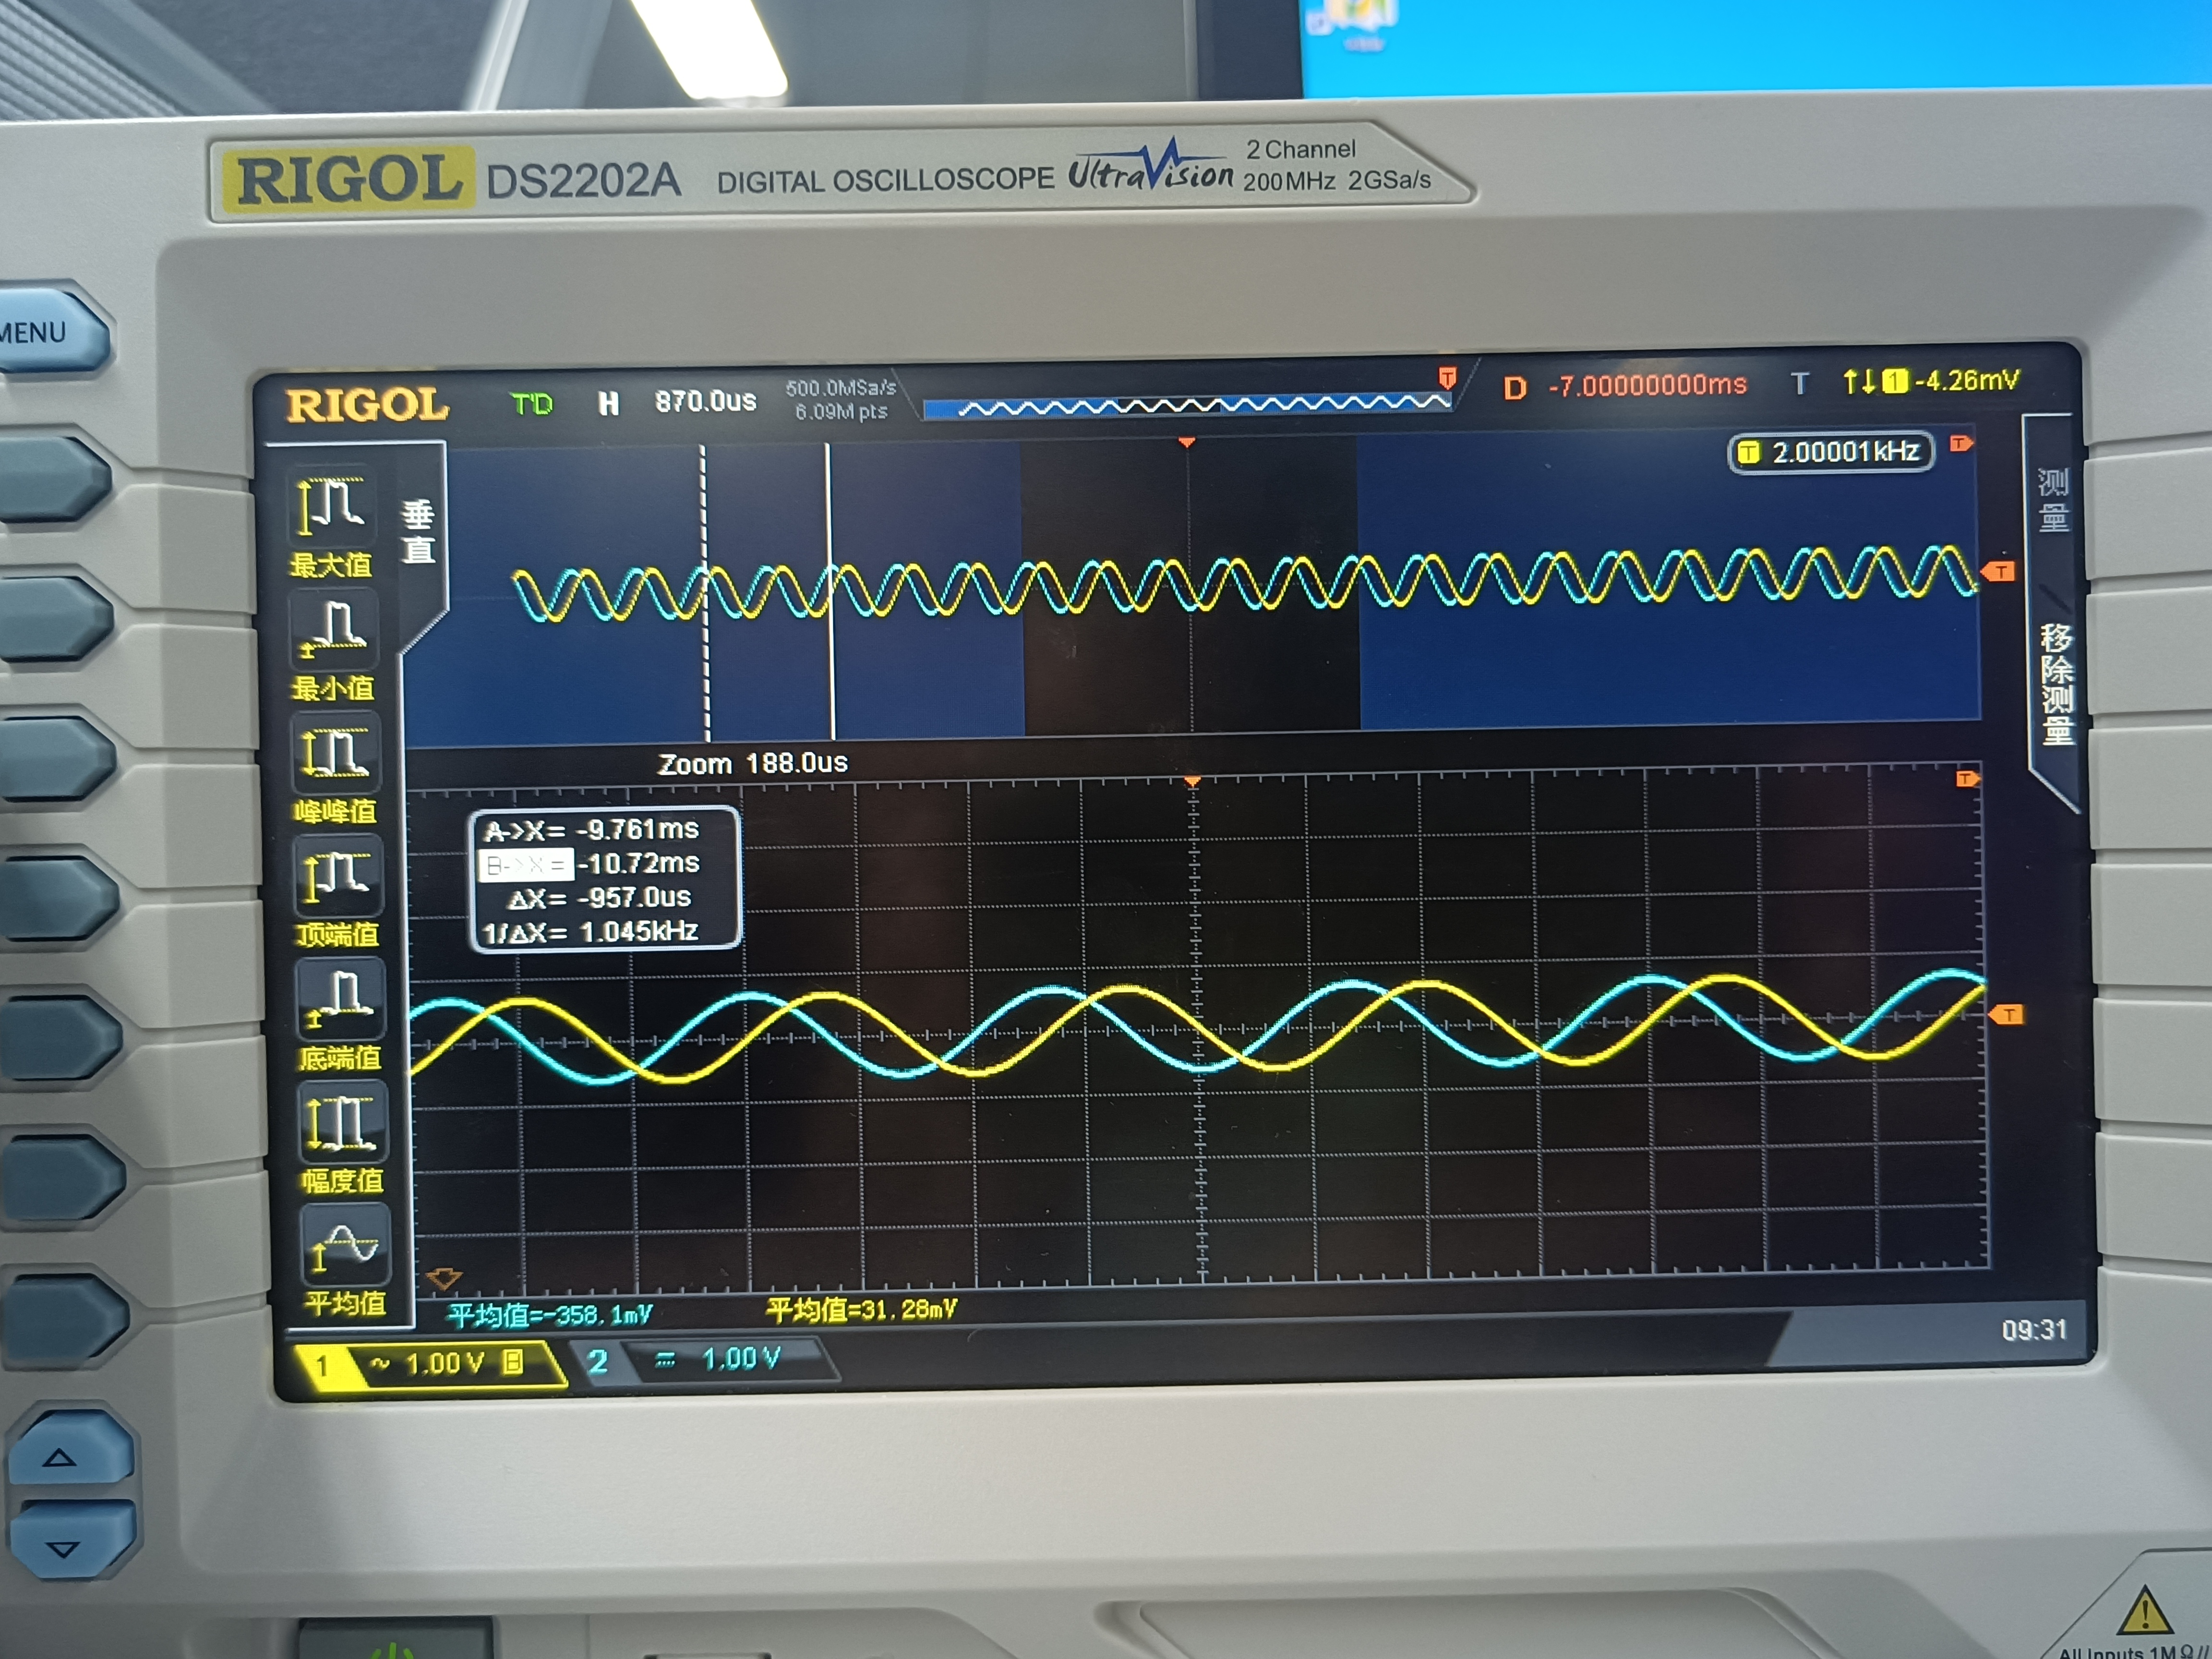
\includegraphics[width=0.32\linewidth]{3.3.2.jpg}}
		\quad
		\subfloat[18dB/oct]{\label{18dB/oct}
		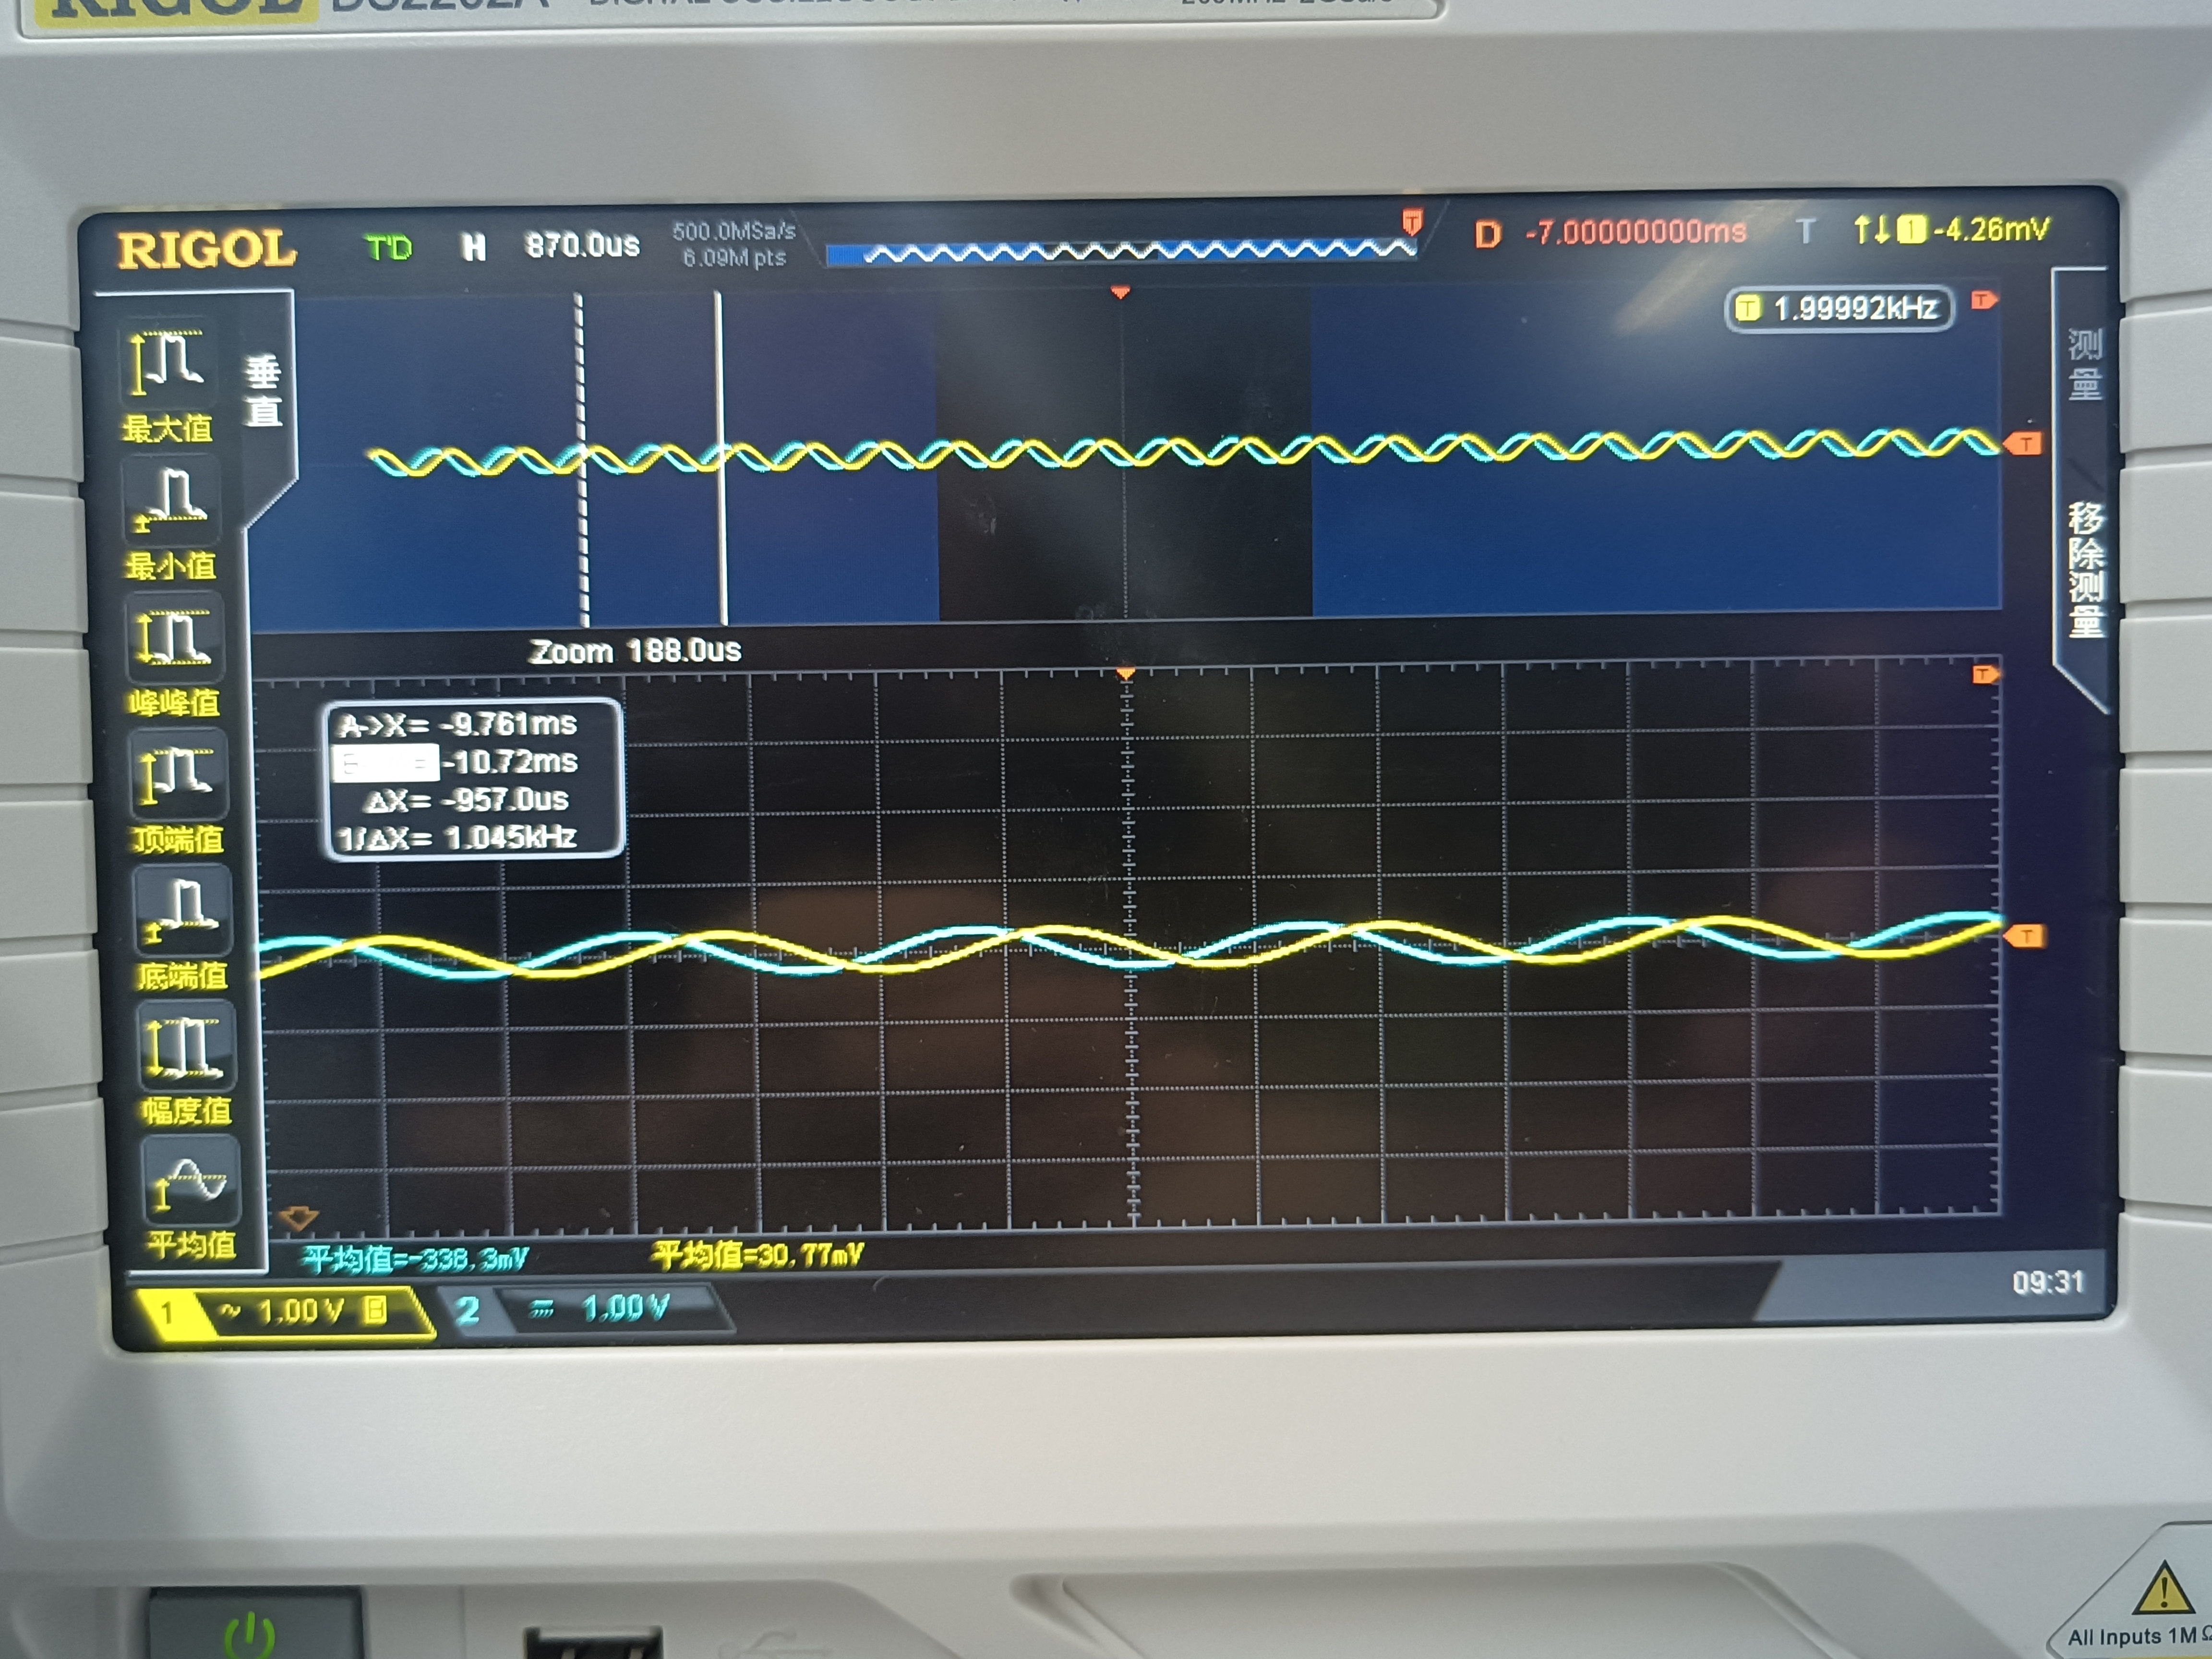
\includegraphics[width=0.32\linewidth]{3.3.3.jpg}}
		\quad
		\subfloat[24dB/oct]{\label{24dB/oct}
		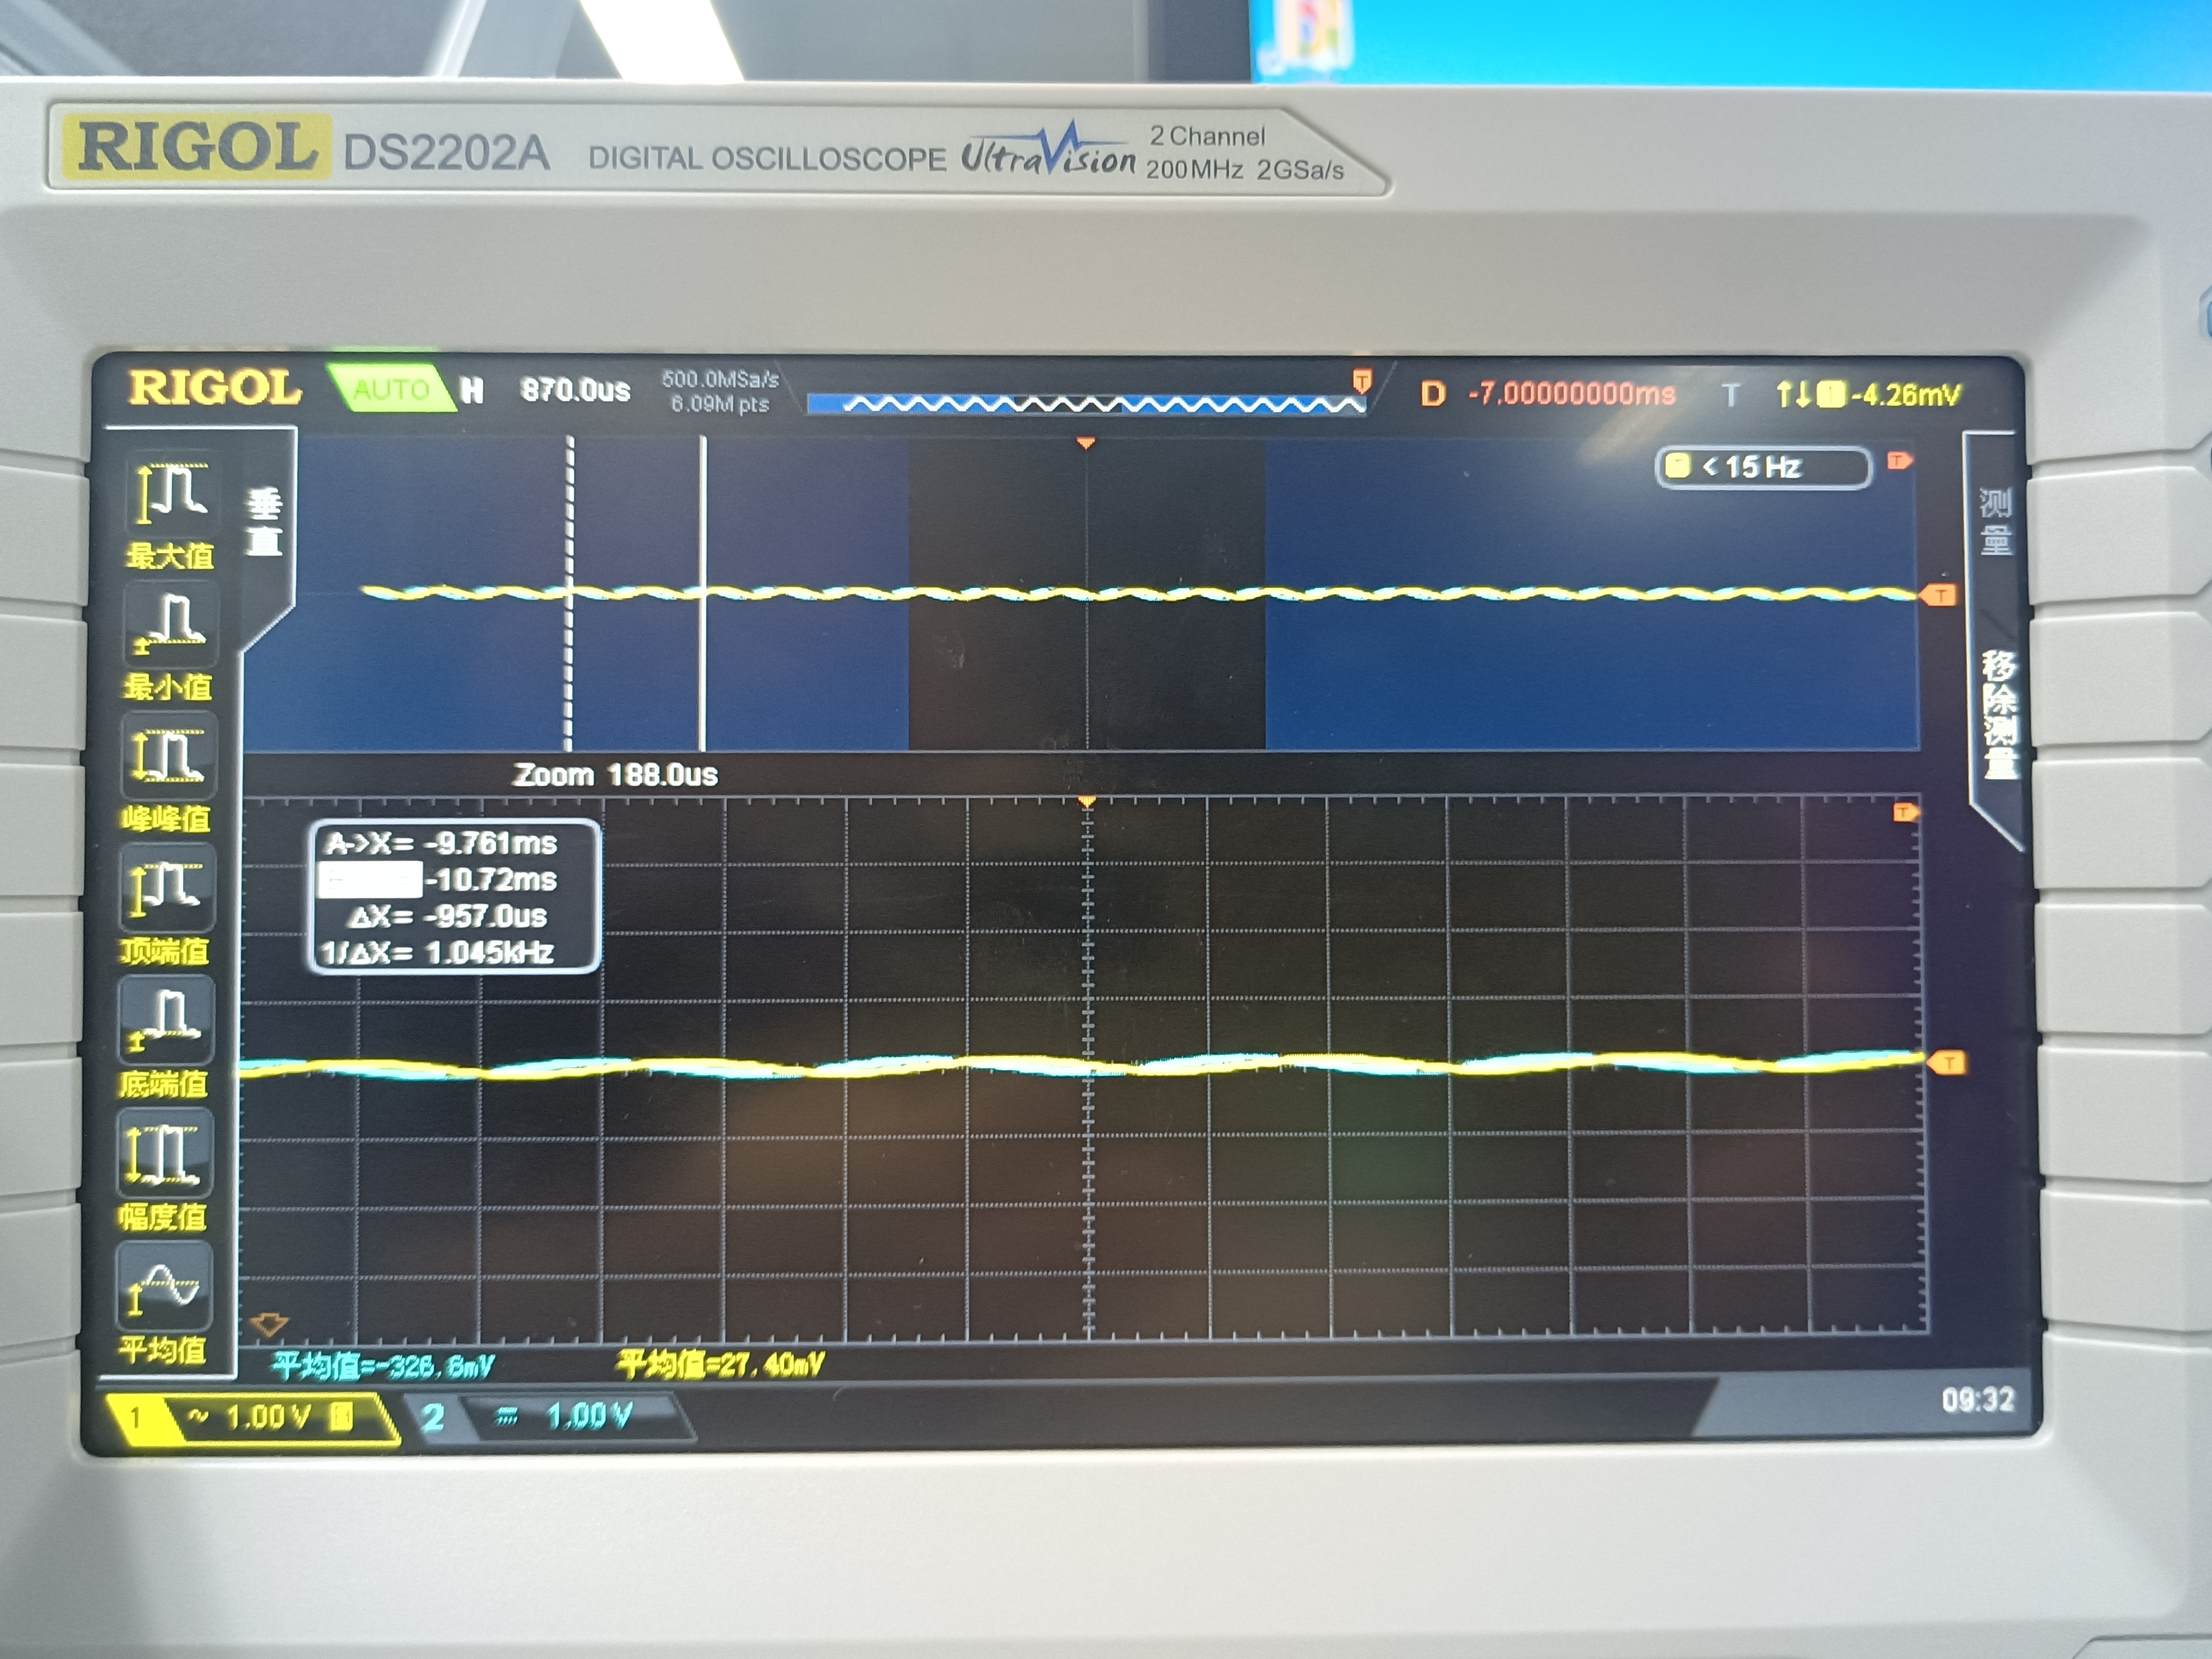
\includegraphics[width=0.32\linewidth]{3.3.4.jpg}}
		\quad
		\caption{时间常数10$\mu$s不变,增大陡降,观察示波器波形}
		\label{时间常数10μs不变,增大陡降,观察示波器波形}
		\end{figure}
		使用  $10\mu s$ 的时间常数,选择时间常数 \( TC \) 等效于选择滤波器的电阻 \( R \) 或电容 \( C \),决定了一阶滤波器的带宽;而选择陡降值则等于选择级联 RC 滤波器的阶数 \( n \),这决定了带通边缘的陡度。

		在 1 阶(6 dB/oct)时,滤波器对高频信号的抑制效果相对较弱,因为其带宽较宽,许多高频成分仍然可以通过。而当提升至 4 阶(24 dB/oct)时,滤波器的陡降增加,使得高频信号在截止频率附近的衰减更加显著。因此,在这种情况下,更多的高频成分被有效削减,输出信号的稳定性和直流分量的增强更加明显。这解释了为何在低阶滤波时滤波效果不明显,而高阶滤波时则能显著改善信号质量。
	\subsection{滤波器带宽对输出信号响应的影响}
	观测输出信号变化 \( R(t) \) 对输入信号变化 (\( \Delta V = V_{sh} - V_{s1} \)) 的响应:

	\begin{enumerate}
		\item 在某一陡降、不同时间常数下;
		\item 在某一时间常数、不同的陡降下。
	\end{enumerate}
	
	
	\begin{question}
		$R(t)$与时间常数和陡降有何关系?
	\end{question}
	\begin{figure}[htbp]
		\centering
		\subfloat[30$\mu$s 24dB/oct]{\label{30us 24dB/oct}
		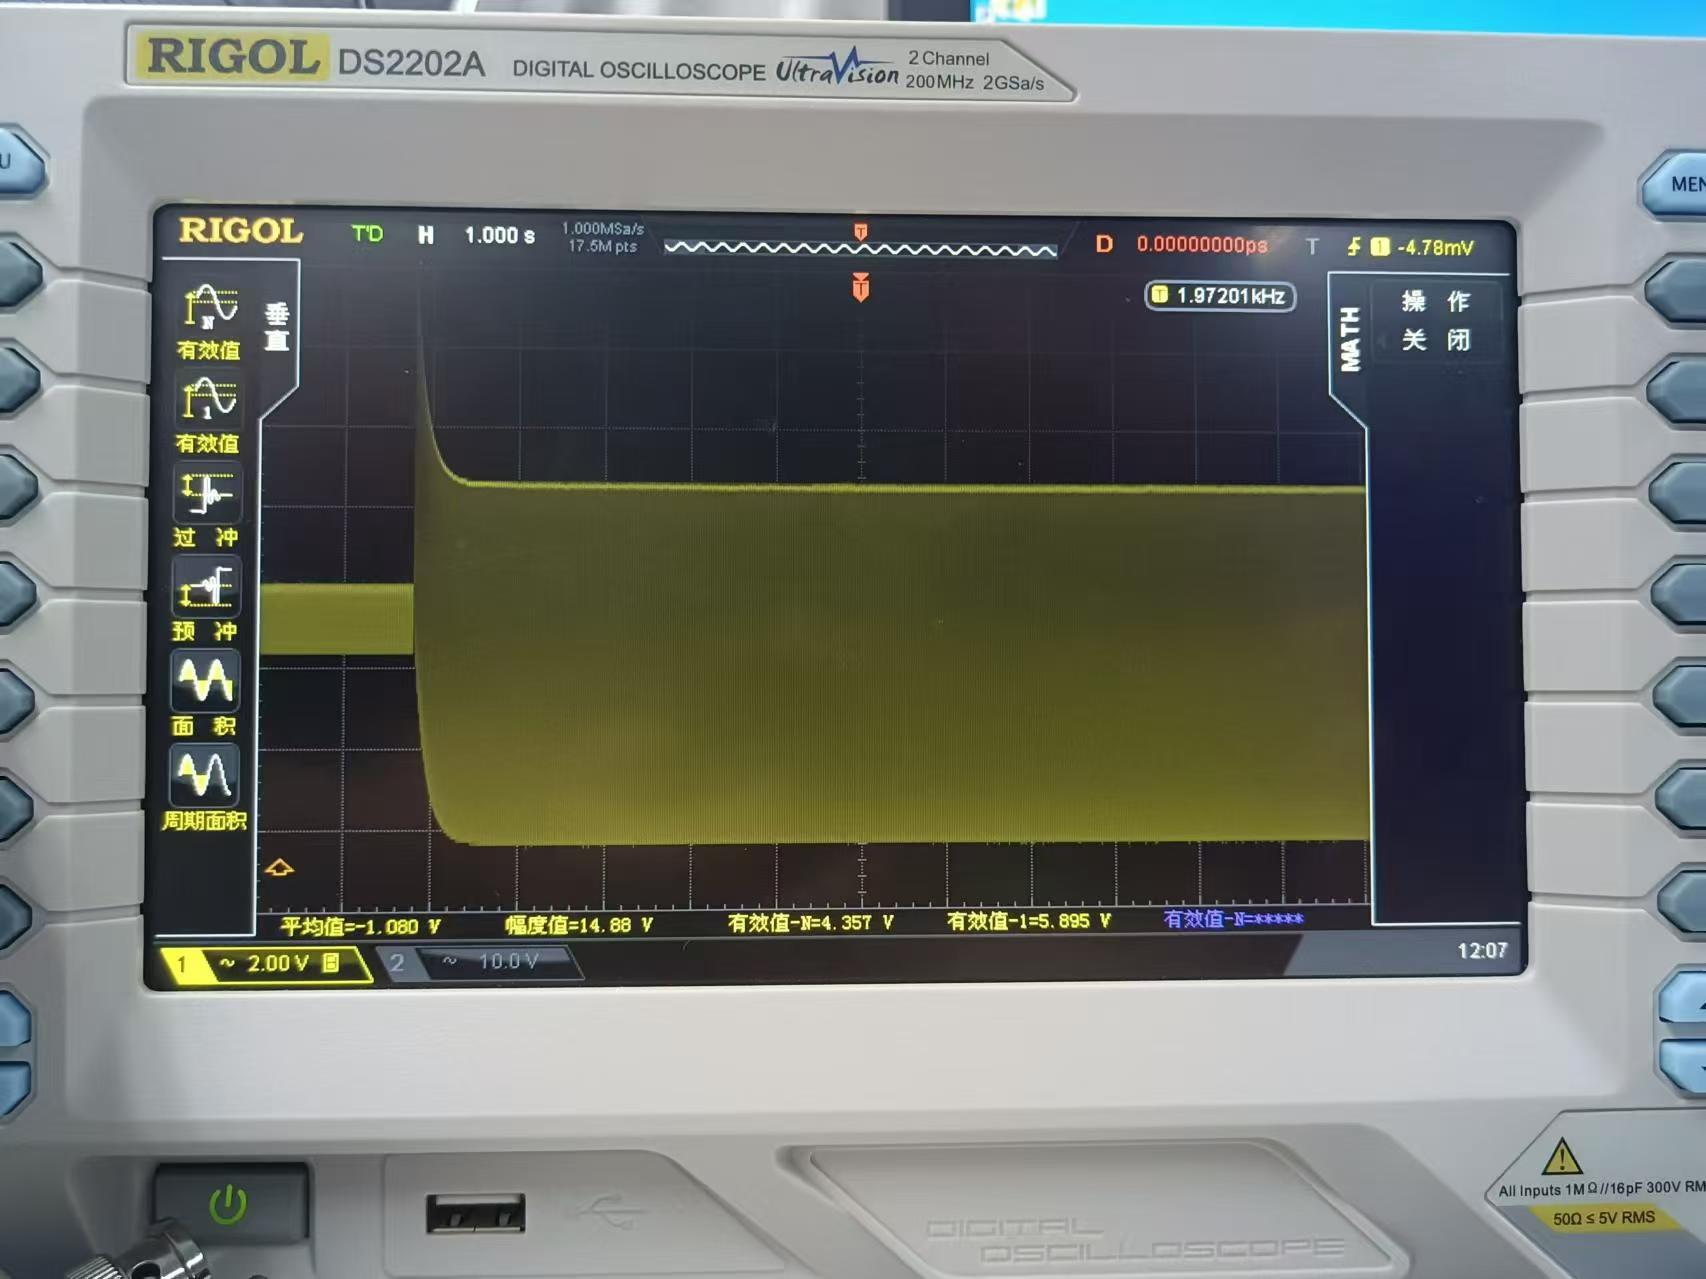
\includegraphics[width=0.32\linewidth]{30us 24.jpg}}
		\quad
		\subfloat[100$\mu$s 24dB/oct]{\label{100us 24dB/oct}
		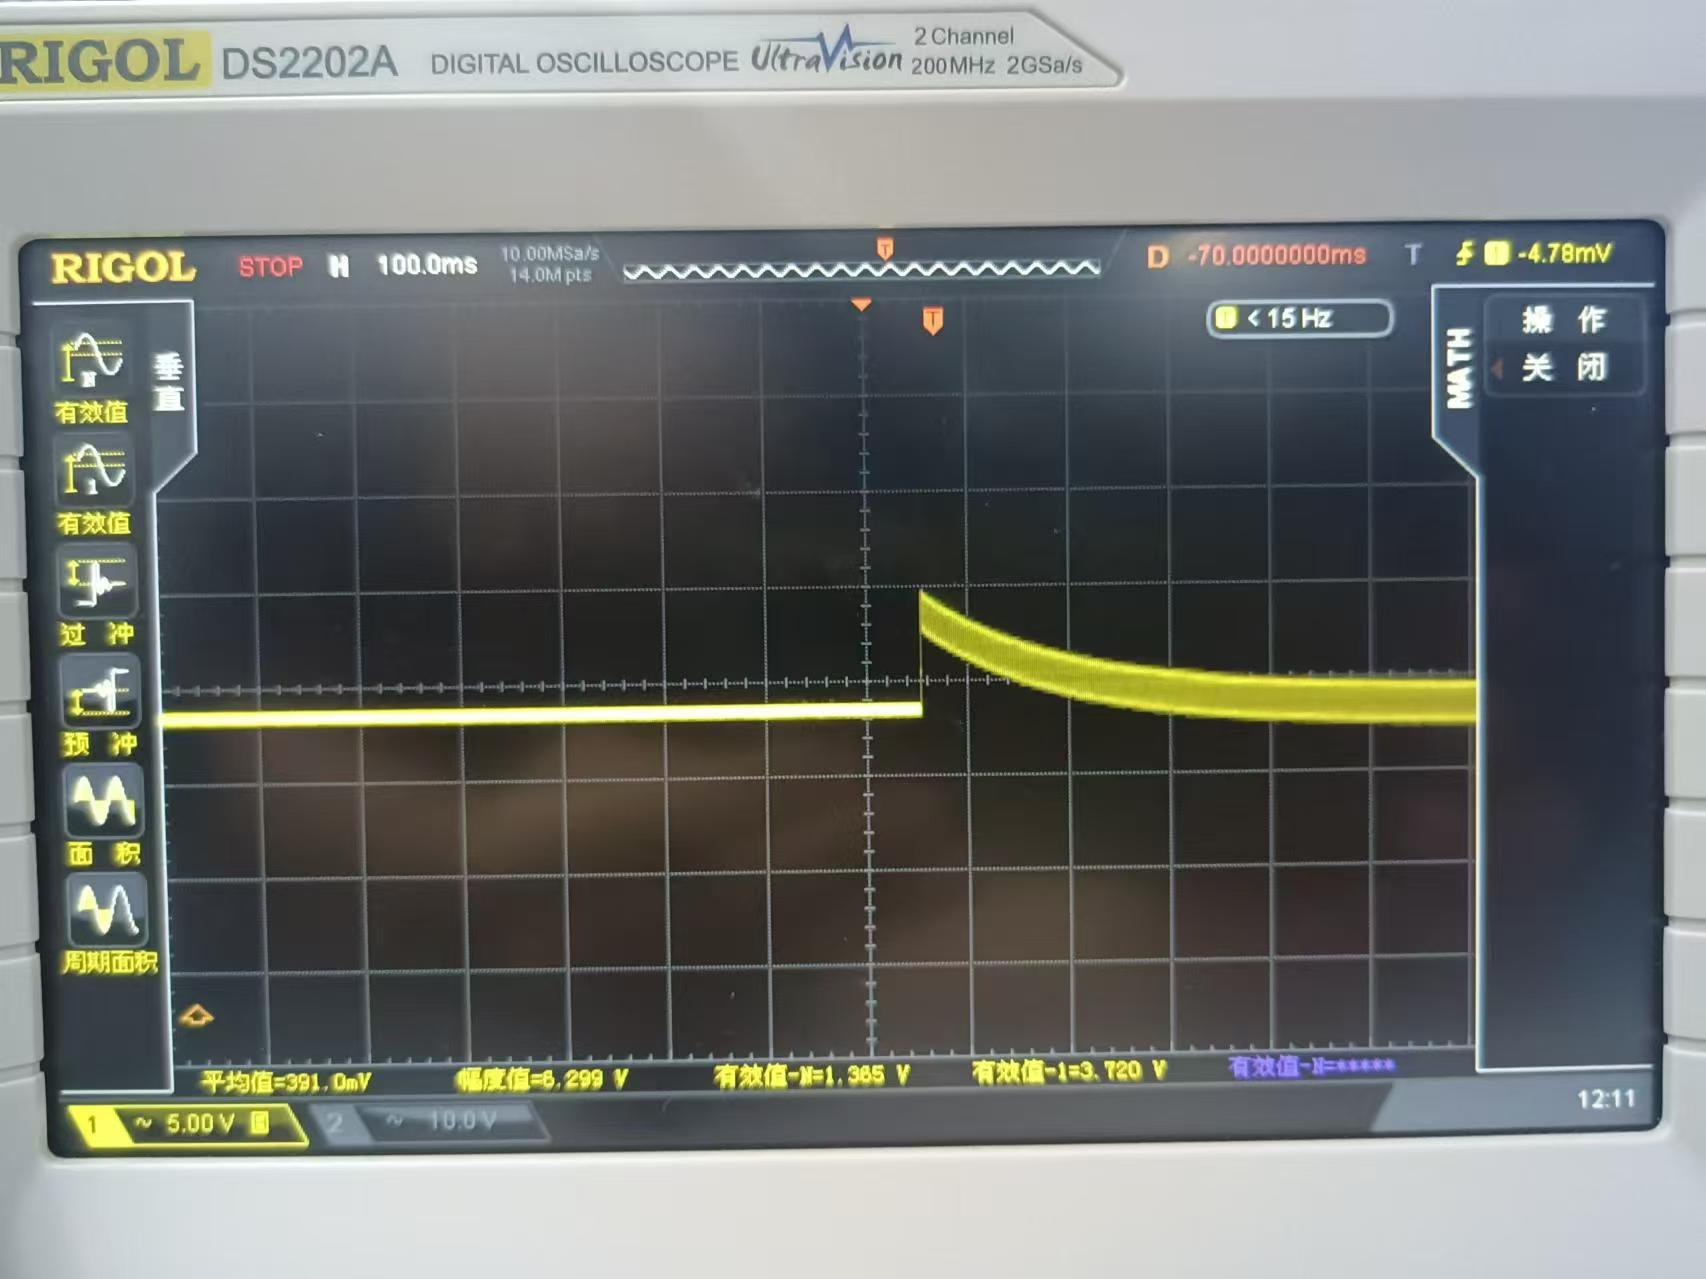
\includegraphics[width=0.32\linewidth]{100us 24.jpg}}
		\quad
		\subfloat[300$\mu$s 24dB/oct]{\label{300us 24dB/oct}
		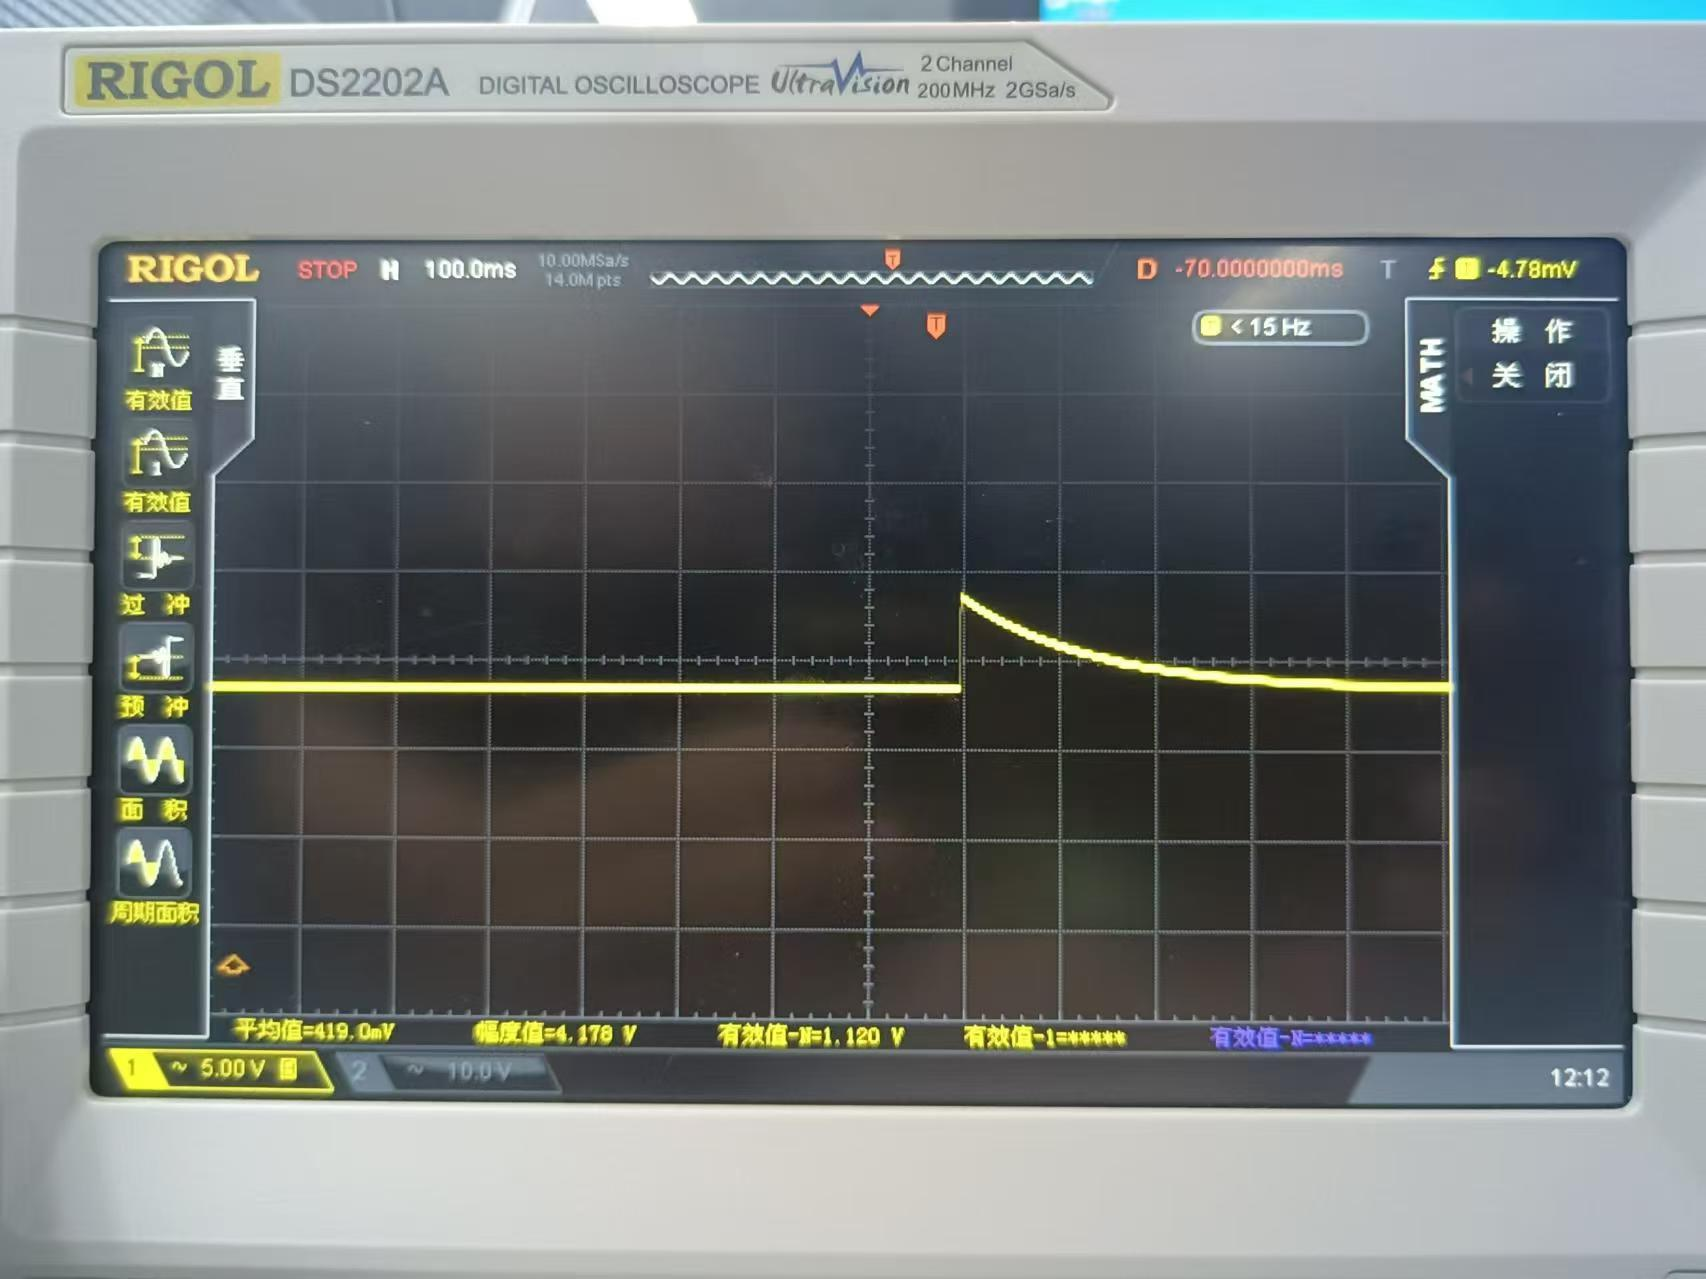
\includegraphics[width=0.32\linewidth]{300us 24.jpg}}
		\quad
		\subfloat[1ms 24dB/oct]{\label{1ms 24dB/oct}
		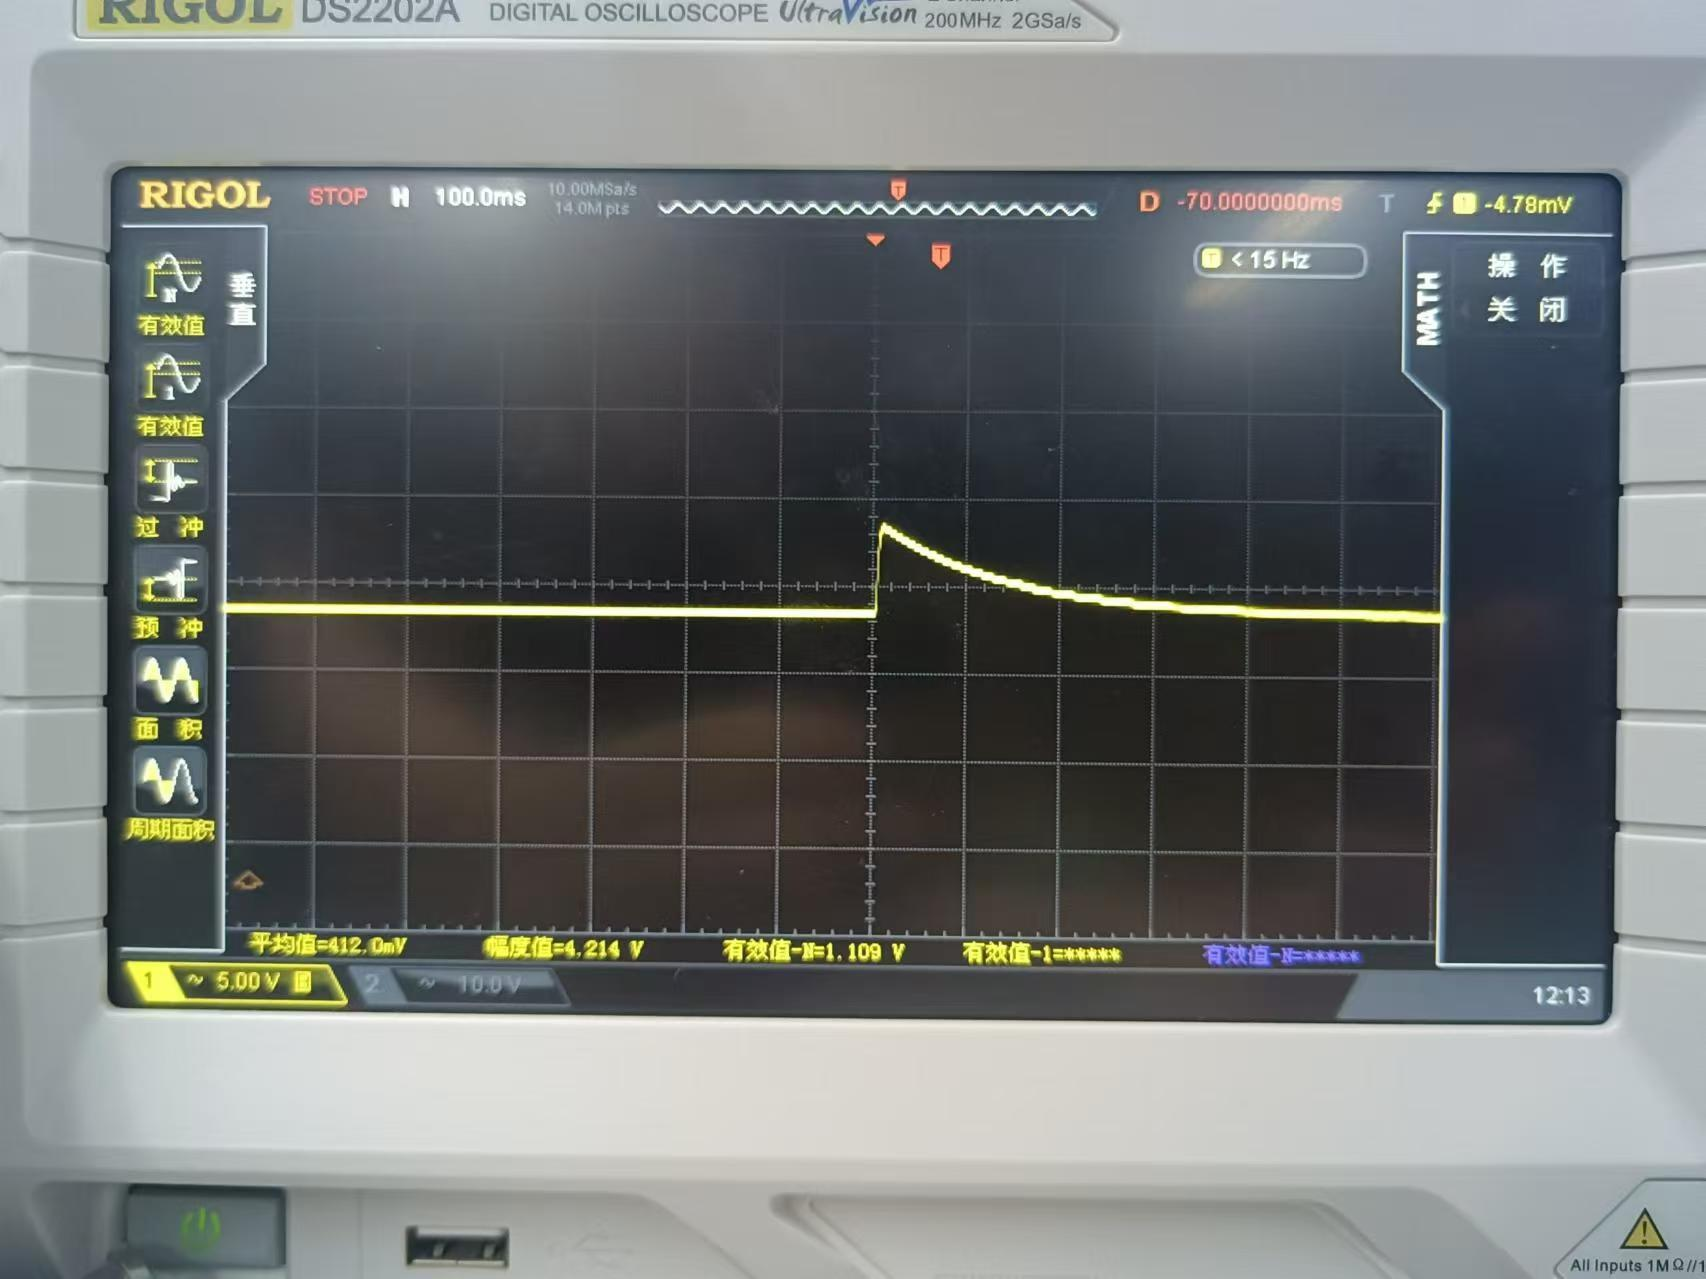
\includegraphics[width=0.32\linewidth]{1ms 24.jpg}}
		\quad
		\caption{陡降为 24dB/oct 不变,改变时间常数}
		\label{陡降为 24dB/oct 不变,改变时间常数}
		\end{figure}

	\begin{figure}[htbp]
		\centering
		\subfloat[100$\mu$s 6dB/oct]{\label{100us 6dB/oct}
		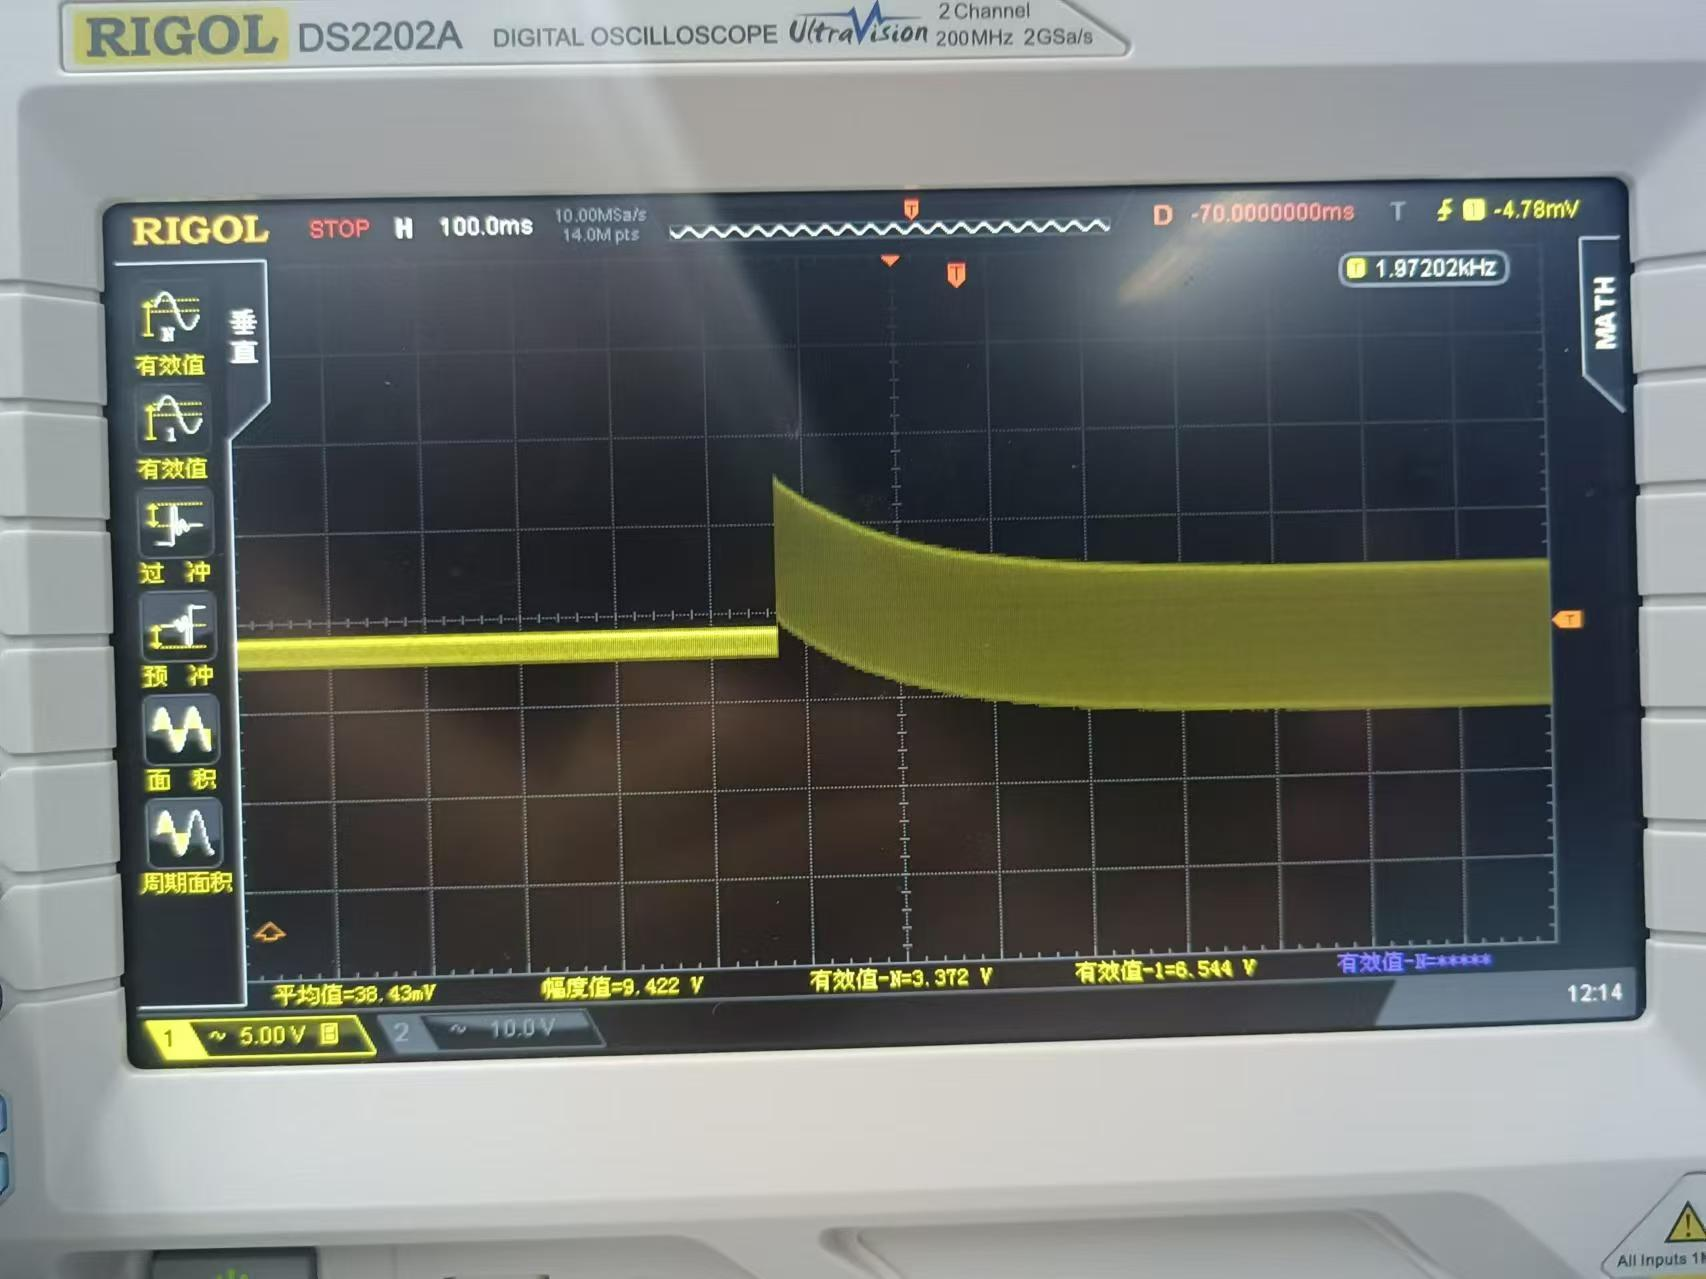
\includegraphics[width=0.32\linewidth]{100us 6.jpg}}
		\quad
		\subfloat[100$\mu$s 12dB/oct]{\label{100us 12dB/oct}
		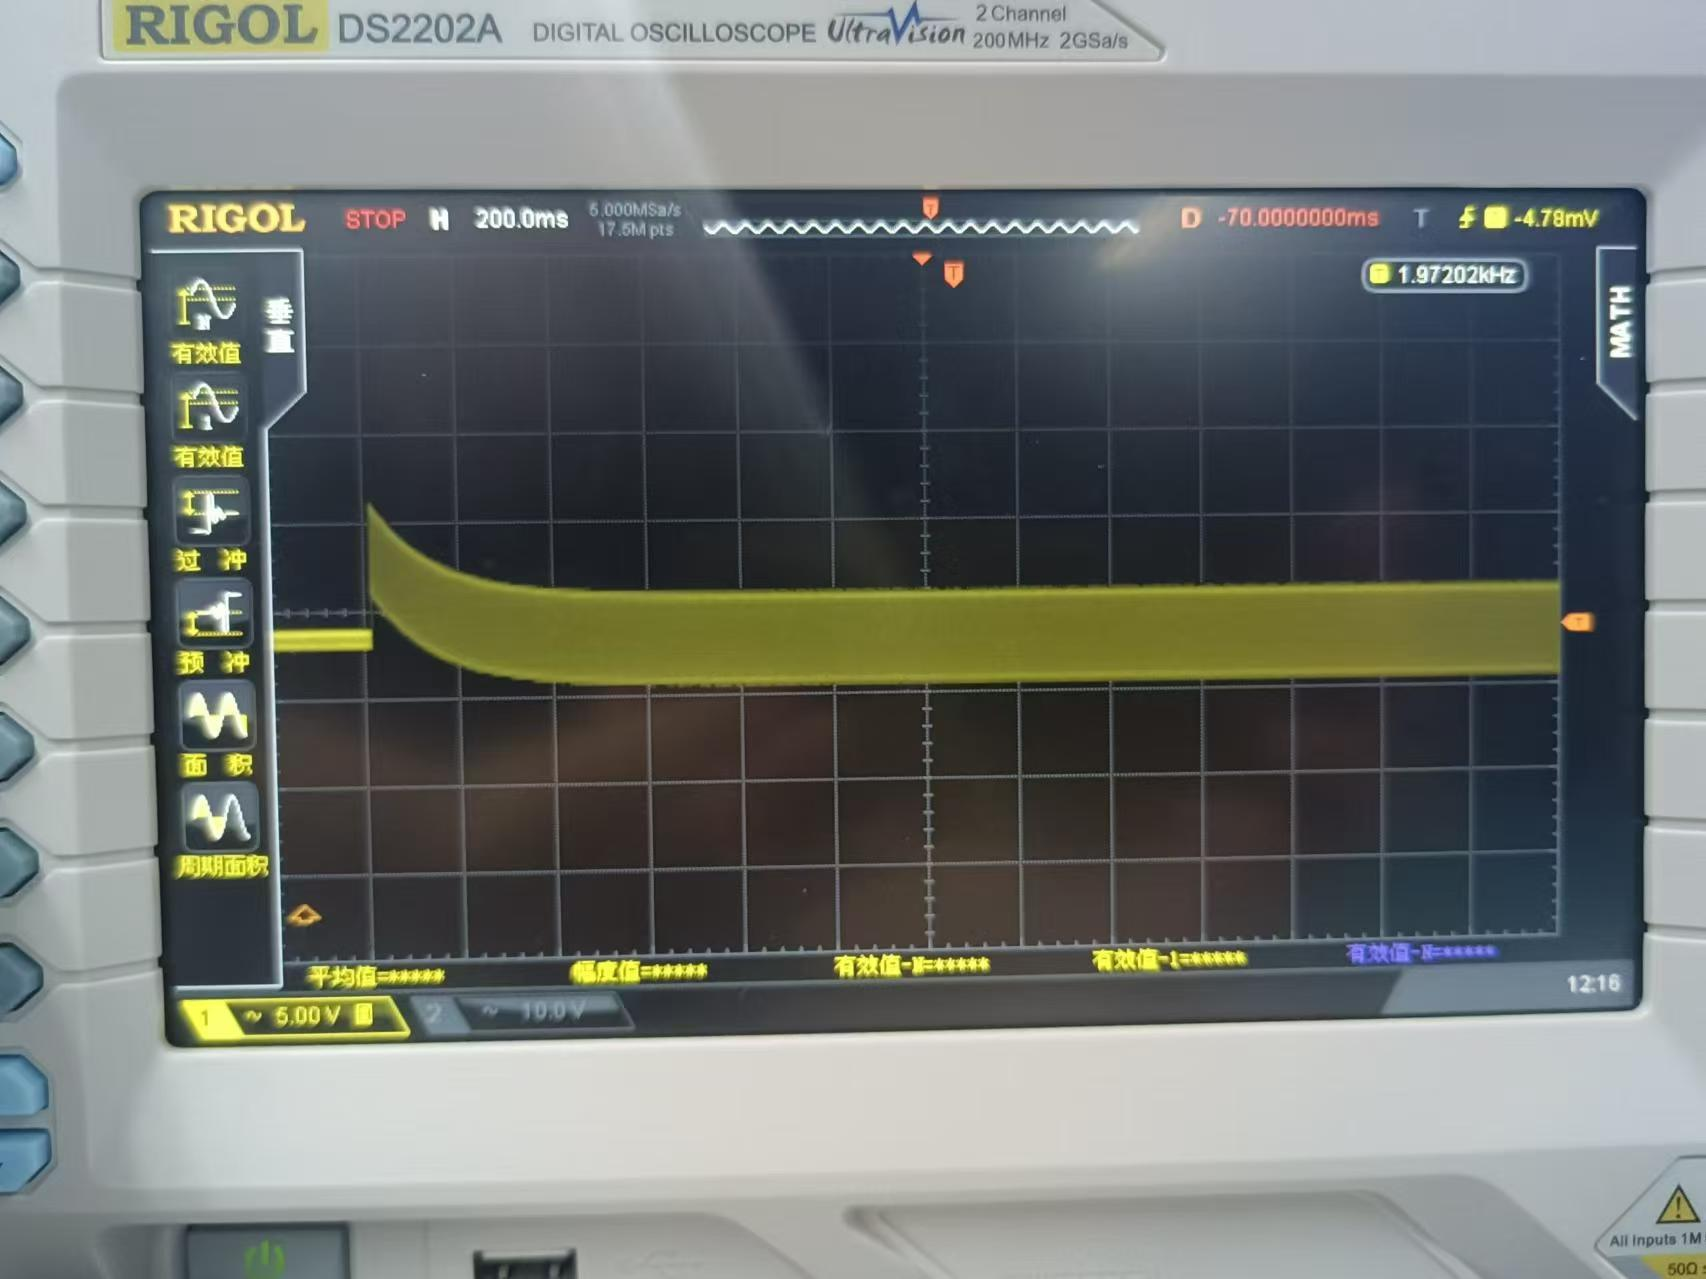
\includegraphics[width=0.32\linewidth]{100us 12.jpg}}
		\quad
		\subfloat[100$\mu$s 18dB/oct]{\label{100us 18dB/oct}
		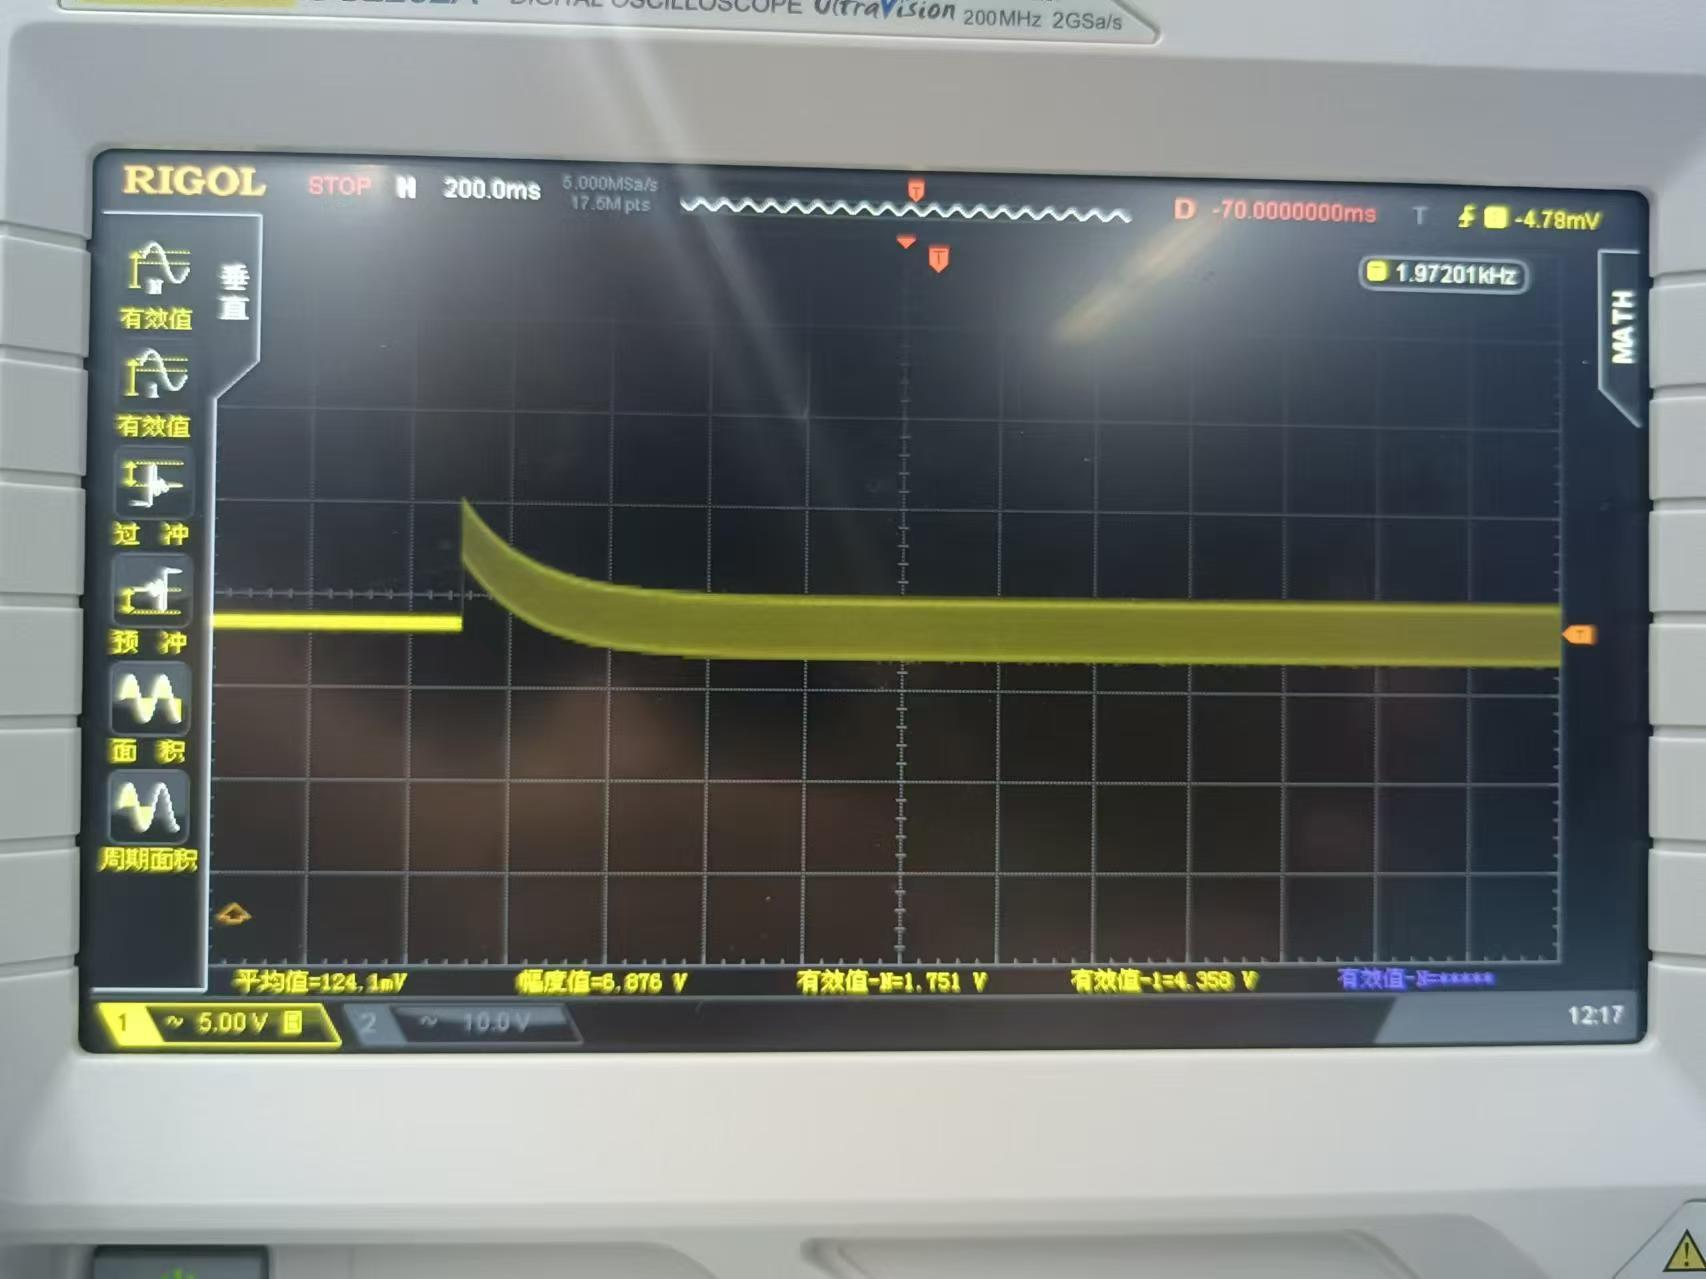
\includegraphics[width=0.32\linewidth]{100us 18.jpg}}
		\quad
		\subfloat[100$\mu$s 24dB/oct]{\label{100us 24dB/oct}
		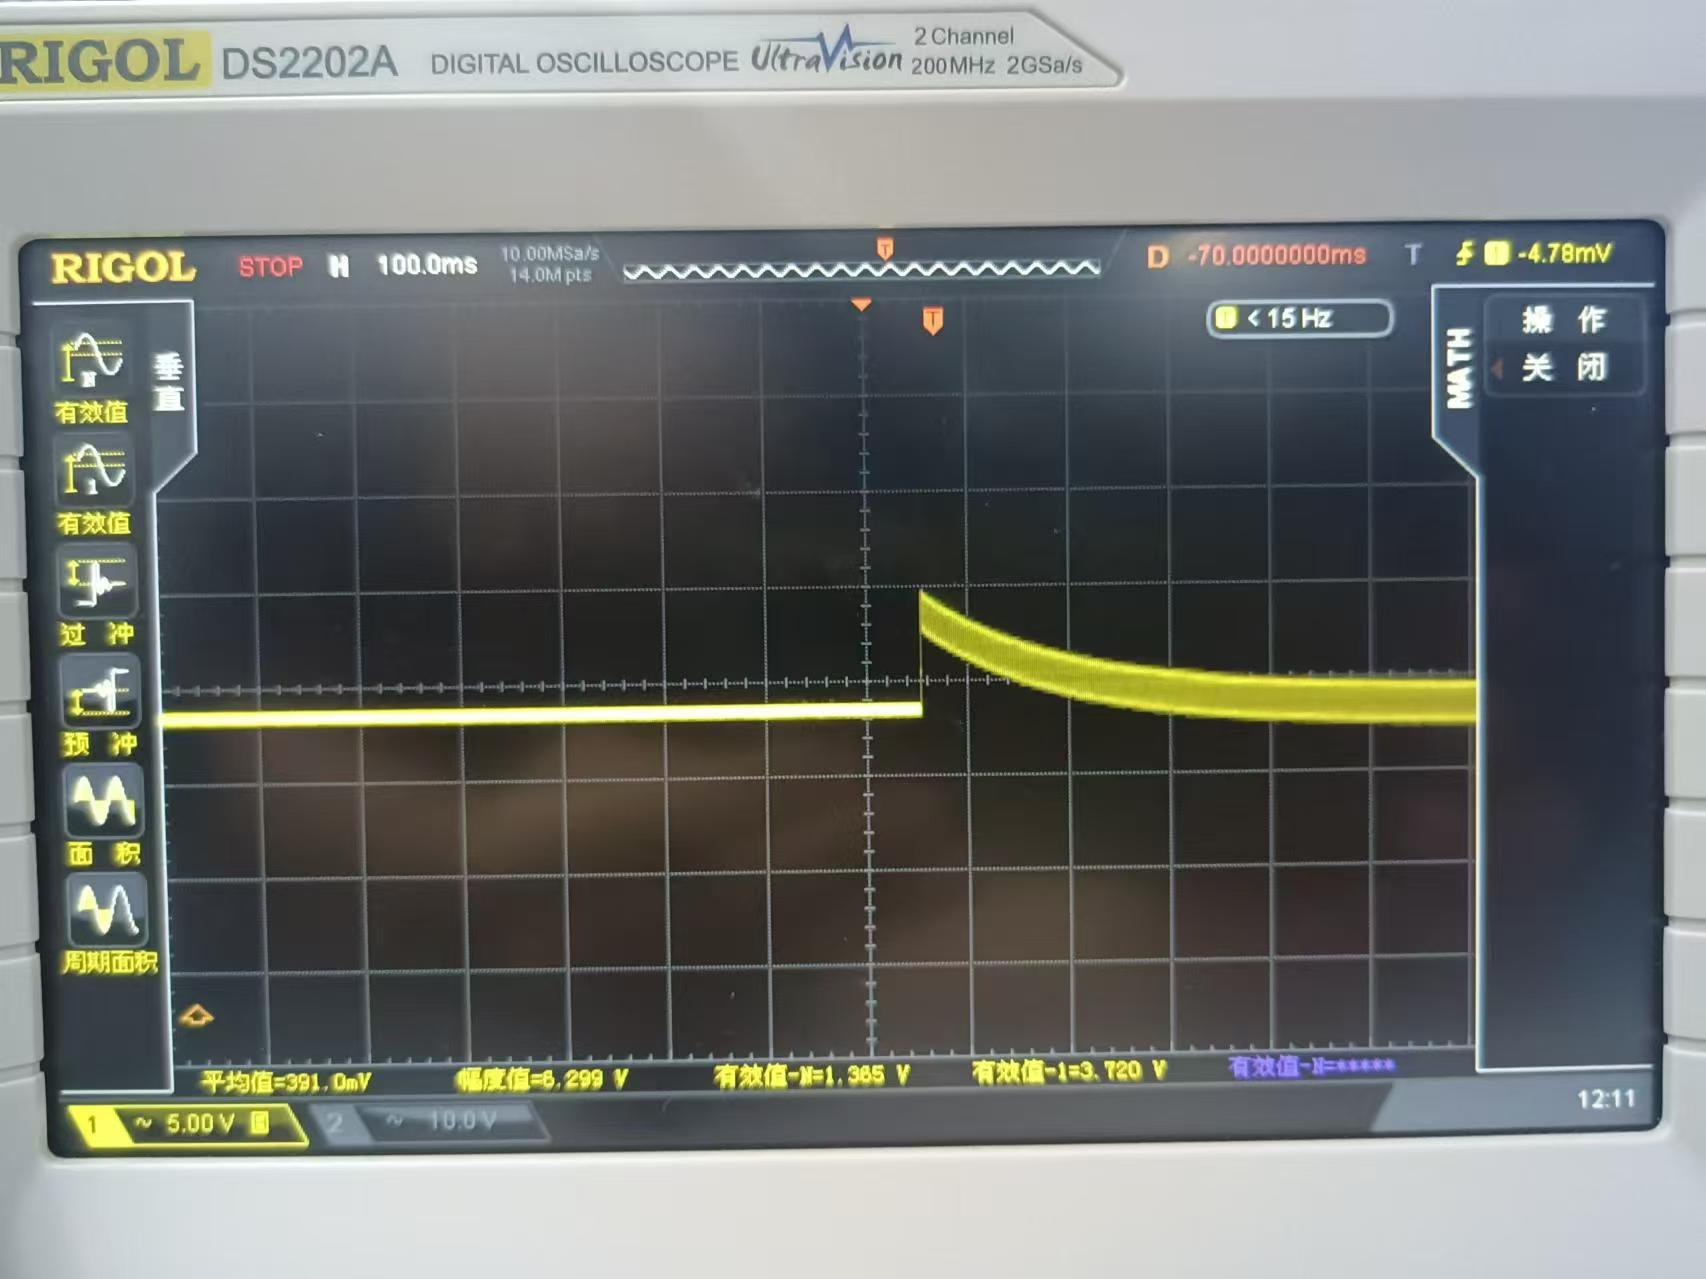
\includegraphics[width=0.32\linewidth]{100us 24.jpg}}
		\quad
		\caption{时间常数为 100$\mu$s 不变,改变陡降}
		\label{时间常数为 100us 不变,改变陡降}
		\end{figure}	
		在保持陡降不变的情况下,随着时间常数从 30 $\mu$s 增加到 1 $ms$,信号变化的幅度会逐渐减小。这是因为较大的时间常数使低通滤波器的通带变窄,从而抑制了高频成分,导致输出信号对快速变化的输入信号响应变得迟缓。虽然增大时间常数可以提高输出信号的稳定性,但这并不意味着时间常数越大越好。对于不同特性的待测信号,选择合适的时间常数至关重要,只有在适当的时间常数下,系统才能具备足够的响应能力,快速捕捉 \( R(t) \) 随时间的变化,确保信号的真实性和有效性。

		在保持时间常数不变的情况下,当陡降从 6 dB/oct 增加到 24 dB/oct 时,信号变化的幅度也会稍微减小。陡降的增加意味着对高频噪声的抑制更加显著,但如果陡降设置过高,可能会导致滤波器对输入信号的响应变得缓慢。这同样影响到对快速变化信号的准确捕捉。因此,选择适当的陡降值是关键,它能够在有效抑制噪声的同时,保证信号变化过程的准确显示。过高的陡降会使得系统对信号变化的敏感度降低,从而影响测量结果的准确性。
		
		总体而言,针对不同变化快慢的待测信号,需要在时间常数和陡降之间找到最佳平衡,以实现最佳的信号捕捉和处理效果。
	\subsection{强噪声背景下的弱信号检测}
\subsubsection{实验步骤}
\begin{enumerate}
    \item 用示波器观察教学实验箱噪声发生器输出的噪声是否为白噪声,记录时域和频域图谱以说明。
    \item 比较 OE1022 与示波器对不同信号强度和信噪比的测量结果,设计如下:
    \begin{enumerate}
        \item 用非市电倍频的频率( 986 Hz),幅值自定的正弦波信号与噪声信号叠加;
        \item 调节锁相放大器的量程灵敏度和 LPF 带宽,获得至少两组稳定的数字读数(3 位有效数字),记录的 \( R \) 值和对应的锁相放大器参数;
        \item 同时在示波器中通过“Math”选项带通滤波器,设置信号频段(通带频率范围),并在滤波后的信号中读取有效值;截录滤波前后的波形图,分别记录所测信号值以及波形图;
        \item 改变 OE1022 产生正弦波有效值,在不同信噪比下重复上述测量;仅要求测量 3 种信噪比的情况,其中必须包括信噪比为 -60 dB 的情况;
        \item 观察滤波效果,分析实验结果。
    \end{enumerate}
\end{enumerate}
\subsubsection{实验准备}
白噪声的定义是:一种随机信号,其特点是包含从低频到高频的所有频率成分,且每个频率的功率均匀分布,听起来如同“嘶嘶”或“沙沙”的声音。其在信号处理和通信领域也常被用于测试和分析系统性能,其数学模型通常被视为零均值的高斯随机过程,具有很高的实用价值。

对于教学实验箱噪声发生器输出的噪声,根据白噪声的定义,下图所显示的噪声的时域和频域图,明显符合关于白噪声的定义,故可以认为教学实验箱噪声发生器输出的噪声是白噪声。
\begin{figure}[htbp]
	\centering
	\includegraphics[width=10cm]{6.1.jpg}
	\caption{利用示波器测量噪声的时域和频域图}
	\label{内利用示波器测量噪声的时域和频域图}
	\end{figure}
	对于此实验中由于要将教学试验箱噪声发生器接入线路中,其中具体接线方式如下所示:
	\begin{figure}[{H}]
		\centering
		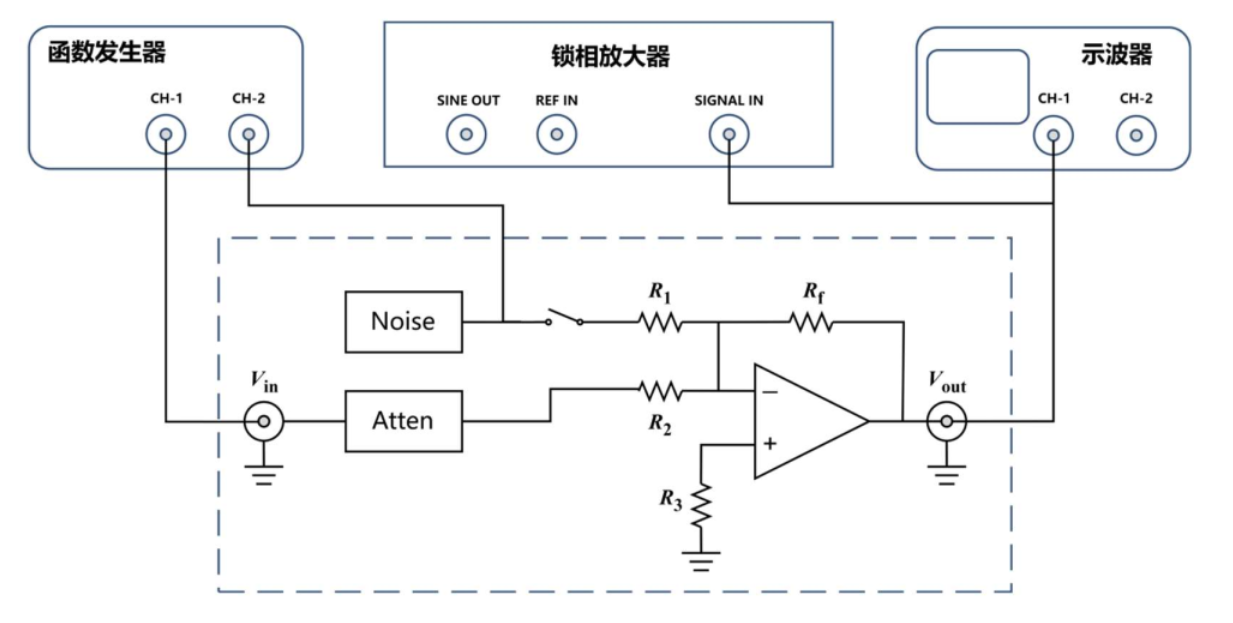
\includegraphics[width=0.8\linewidth]{jiexian.png}
		\caption{实验接线示意图}
		\label{}
	\end{figure}
	\begin{figure}[{H}]
		\centering
		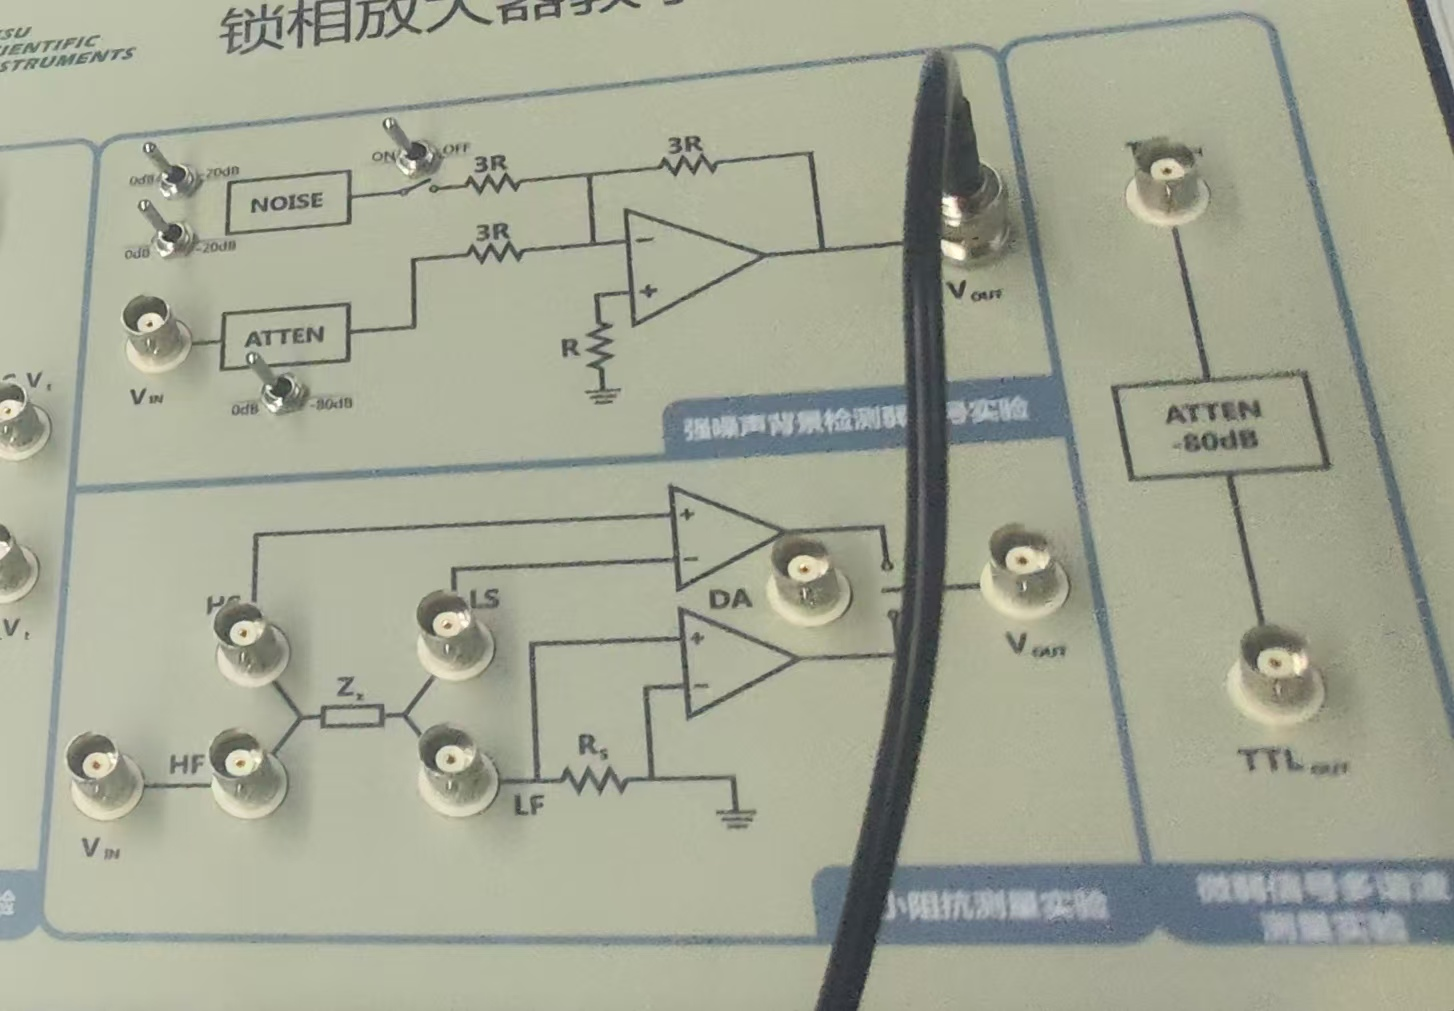
\includegraphics[width=0.8\linewidth]{噪声箱.jpg}
		\caption{}
		\label{}
	\end{figure}
	\begin{question}
		如何获得幅值为 $0.1mVrms $的正弦波输入信号?
	\end{question}
直接通过信号发生器输入即可,这个精度的信号,信号发生器可以生成,再小精度的信号的生成方式在讨论正弦波幅值时进行讨论。
\begin{question}
	对低信噪比信号或非周期噪声测量,能否用示波器的“auto”键?若通过手动调节,示波器屏宽(时间轴范围)应为多少个信号周期为宜?
\end{question}
对于低信噪比信号或非周期噪声的测量,使用示波器的“auto”键可能会导致无法准确捕捉到信号的细节。因为“auto”模式通常会根据输入信号的特征自动调整设置,但在低信噪比情况下,这可能会影响波形的显示。

手动调节示波器时,建议将屏幕的时间轴范围设置为多个信号周期,以便更好地观察信号的形态。一般而言,设置为2到5个信号周期是比较合适的,这样可以平衡信号的可见性和波形的完整性。如果信号周期较短,可以适当缩短时间轴范围,但仍然需要保证至少包含1到2个完整周期的波形以便进行分析。

	\begin{question}
		对低信噪比信号或非周期噪声测量,能否用示波器的“auto”键?若通过手动调节,示波器屏宽(时间轴范围)应为多少个信号周期为宜?
	\end{question}
\begin{enumerate}
	\item  精确测量:有效值(RMS)是信号在一个周期内的功率等效值。如果时间轴范围不足以包含完整周期,可能会导致测量的不准确,因为示波器无法捕捉到信号的全部特性。
	\item  避免混叠:如果时间轴范围不完整,信号可能会与下一个周期的信号重叠,导致混叠现象,进一步影响有效值的计算。
	\item 稳定显示:显示完整周期有助于观察信号的稳定性和重复性,使得波形更加平滑,从而便于分析信号特征。
	\item 周期性特征:信号的有效值计算通常依赖于其周期性特征,只有在完整周期内进行测量才能获得准确的结果。
\end{enumerate}

	
\begin{question}
	用锁相放大器测量 R 值时,读数应保留几位有效数字?调节锁相放大器的什么参数设置可以得到?调节锁相放大器的什么参数可以获得稳定的读数。
\end{question}
应该保留两位数字,通过调节锁相放大器的量程灵敏度(sensitivity),便可以调节读数的有效位数,按照实验经验,正常来说读数较为稳定。
\subsubsection{实验数据解析}
在记录实验数据之前,需要明确在实验数据记录表中各个数据所代表的含义。

一切实验的基础是信噪比公式:$$\mathrm{SNR_{i}(dB)}=20lg(V_{S,RMS}/V_{N,RMS})$$

输入信号信噪比:这个要提前设定好,根据此信噪比来设定其他参数。

\textbf{示波器:}
\begin{enumerate}
	\item 正弦波 $V_{in}$幅值:这个需要根据,设定的信噪比以及实际的噪声信号的大小而定。
	\item 噪声信号大小:由于存在仪器老化,尽管教学实验箱噪声发生器的标准发出的噪声为$100mV_{rms}$,但是实际上存在偏差,需要测出一个实际值记录。
	\item $\mathrm{SNR_i}$:此信噪比相比于设定的输入信号信噪比会存在些许的不同,这是由于实验设定值会存在一定的误差,故存在不同。

	\item 滤波器带宽:带宽的计算是在设置示波器的数字滤波是,会给出一个频率上限和下限,将两者相减便可以得到带宽。
	\item 滤波后的信号有效值:在示波器上,使用滤波后会有一条紫色的线,这就是滤波后的信号,测得此信号的有效值即可。
	\item $SNR_{0,0S}$:滤波后的信号的和噪声有一个新的信噪比,由于是示波器的滤波后的信噪比,故为:os。
\end{enumerate}
\textbf{锁相放大器:}
\begin{enumerate}
	\item 量程灵敏度:通过设置量程灵敏度,可以调整数值的精度,所以选择合适的灵敏度,可以既保证了量程满足输出的数值要求,也保证了一定的精度。
	\item 时间常数:由设置的频率计算而来。
	\item 陡降:同样为预先设置。
	\item LPF带宽:需要通过计算得来,根据不同的陡降得到不同的系数,在乘以时间常数的倒数便得到带宽。
	\item 信号有效值R:可以通过锁相放大器面板直接输出。
	\item 噪声测量值N:可以通过锁相放大器面板直接输出。
	\item  $SNR_{0,0l}$:滤波后的信号的和噪声有一个新的信噪比,由于是锁相放大器的滤波后的信噪比,故为:ol。
\end{enumerate}
根据以上的相关参数的设置要求,最终测得以下数据,其中关于待测信号的波形图未在表格中,已附在后面。

需要注意的是,在$-80dB$的情况,由于输入信号无法到达该信噪比的要求的数值,故打开在噪声发生器上$-80dB$的开关,从而完成实验。




\begin{table}[H]
	\centering
	\caption{强噪声背景检测弱信号实验记录}
	\label{tab:tab1}
	\begin{tabular}{|c|c|c|c|c|c|}
		\hline
		\thead{仪\\器} & 输入信号信噪比 & (dB) & 0 & -30 & -80 \\
		\hline
		\multirow{7}{*}{\thead{示\\波\\器}} & 正弦波$V_{in}$幅值 & (mVrms) & 101 & 3.25 & 0.01 \\
		\cline{2-6}
		\multirow{7}{*}{} & 噪声信号大小 & (mVrms) & 101.23 & 101.23 & 101.23 \\
		\cline{2-6}
		\multirow{7}{*}{} & SNR$_i$ & (dB) & -0.0197 & 29.86 & -80.11 \\
		\cline{2-6}
		
		\cline{2-6}
		\multirow{7}{*}{} & 滤波器带宽 & (Hz) & 407 & 407 & 407 \\
		\cline{2-6}
		\multirow{7}{*}{} & 滤波后信号有效值 & (mVrms) & 89.59 & 3.65 & 2.792 \\
		\cline{2-6}
		\multirow{7}{*}{} & $SNR_oos$ & (dB) & -1.06 & -28.8 & -37.18 \\
		\hline
		\multirow{7}{*}{\thead{锁\\相\\放\\大\\器}} & 量程灵敏度 & (mV) & 200 & 200 & 200 \\
		\cline{2-6}
		\multirow{7}{*}{} & 时间常数 & (ms) & 1 & 1 & 1 \\
		\cline{2-6}
		\multirow{7}{*}{} & 陡降 & dB/oct & 24 & 24 & 24 \\
		\cline{2-6}
		\multirow{7}{*}{} & LPF带宽 & (Hz) & 78.625 & 78.625 & 78.625 \\
		\cline{2-6}
		\multirow{7}{*}{} & 信号有效值R & (mVrms) & 100.39 & 3.29 & 0.31 \\
		\cline{2-6}
		\multirow{7}{*}{} & 滤波后信号有效值 & (mVrms) & 0.03 & 0.03 & 0.03 \\
		\cline{2-6}
		\multirow{7}{*}{} & SNR$_{o,lo}$ & (dB) & 70 & 40 & 20.28 \\
		\hline
	\end{tabular}
\end{table}		
\begin{figure}[H]
	\centering
	\includegraphics[width=10cm]{6.1.jpg}
	\caption{利用示波器测量噪声的时域和频域图}
	\label{内利用示波器测量噪声的时域和频域图}
	\end{figure}

	\begin{figure}[htbp]
		\centering
		\subfloat[-30dB]{\label{6.2}
		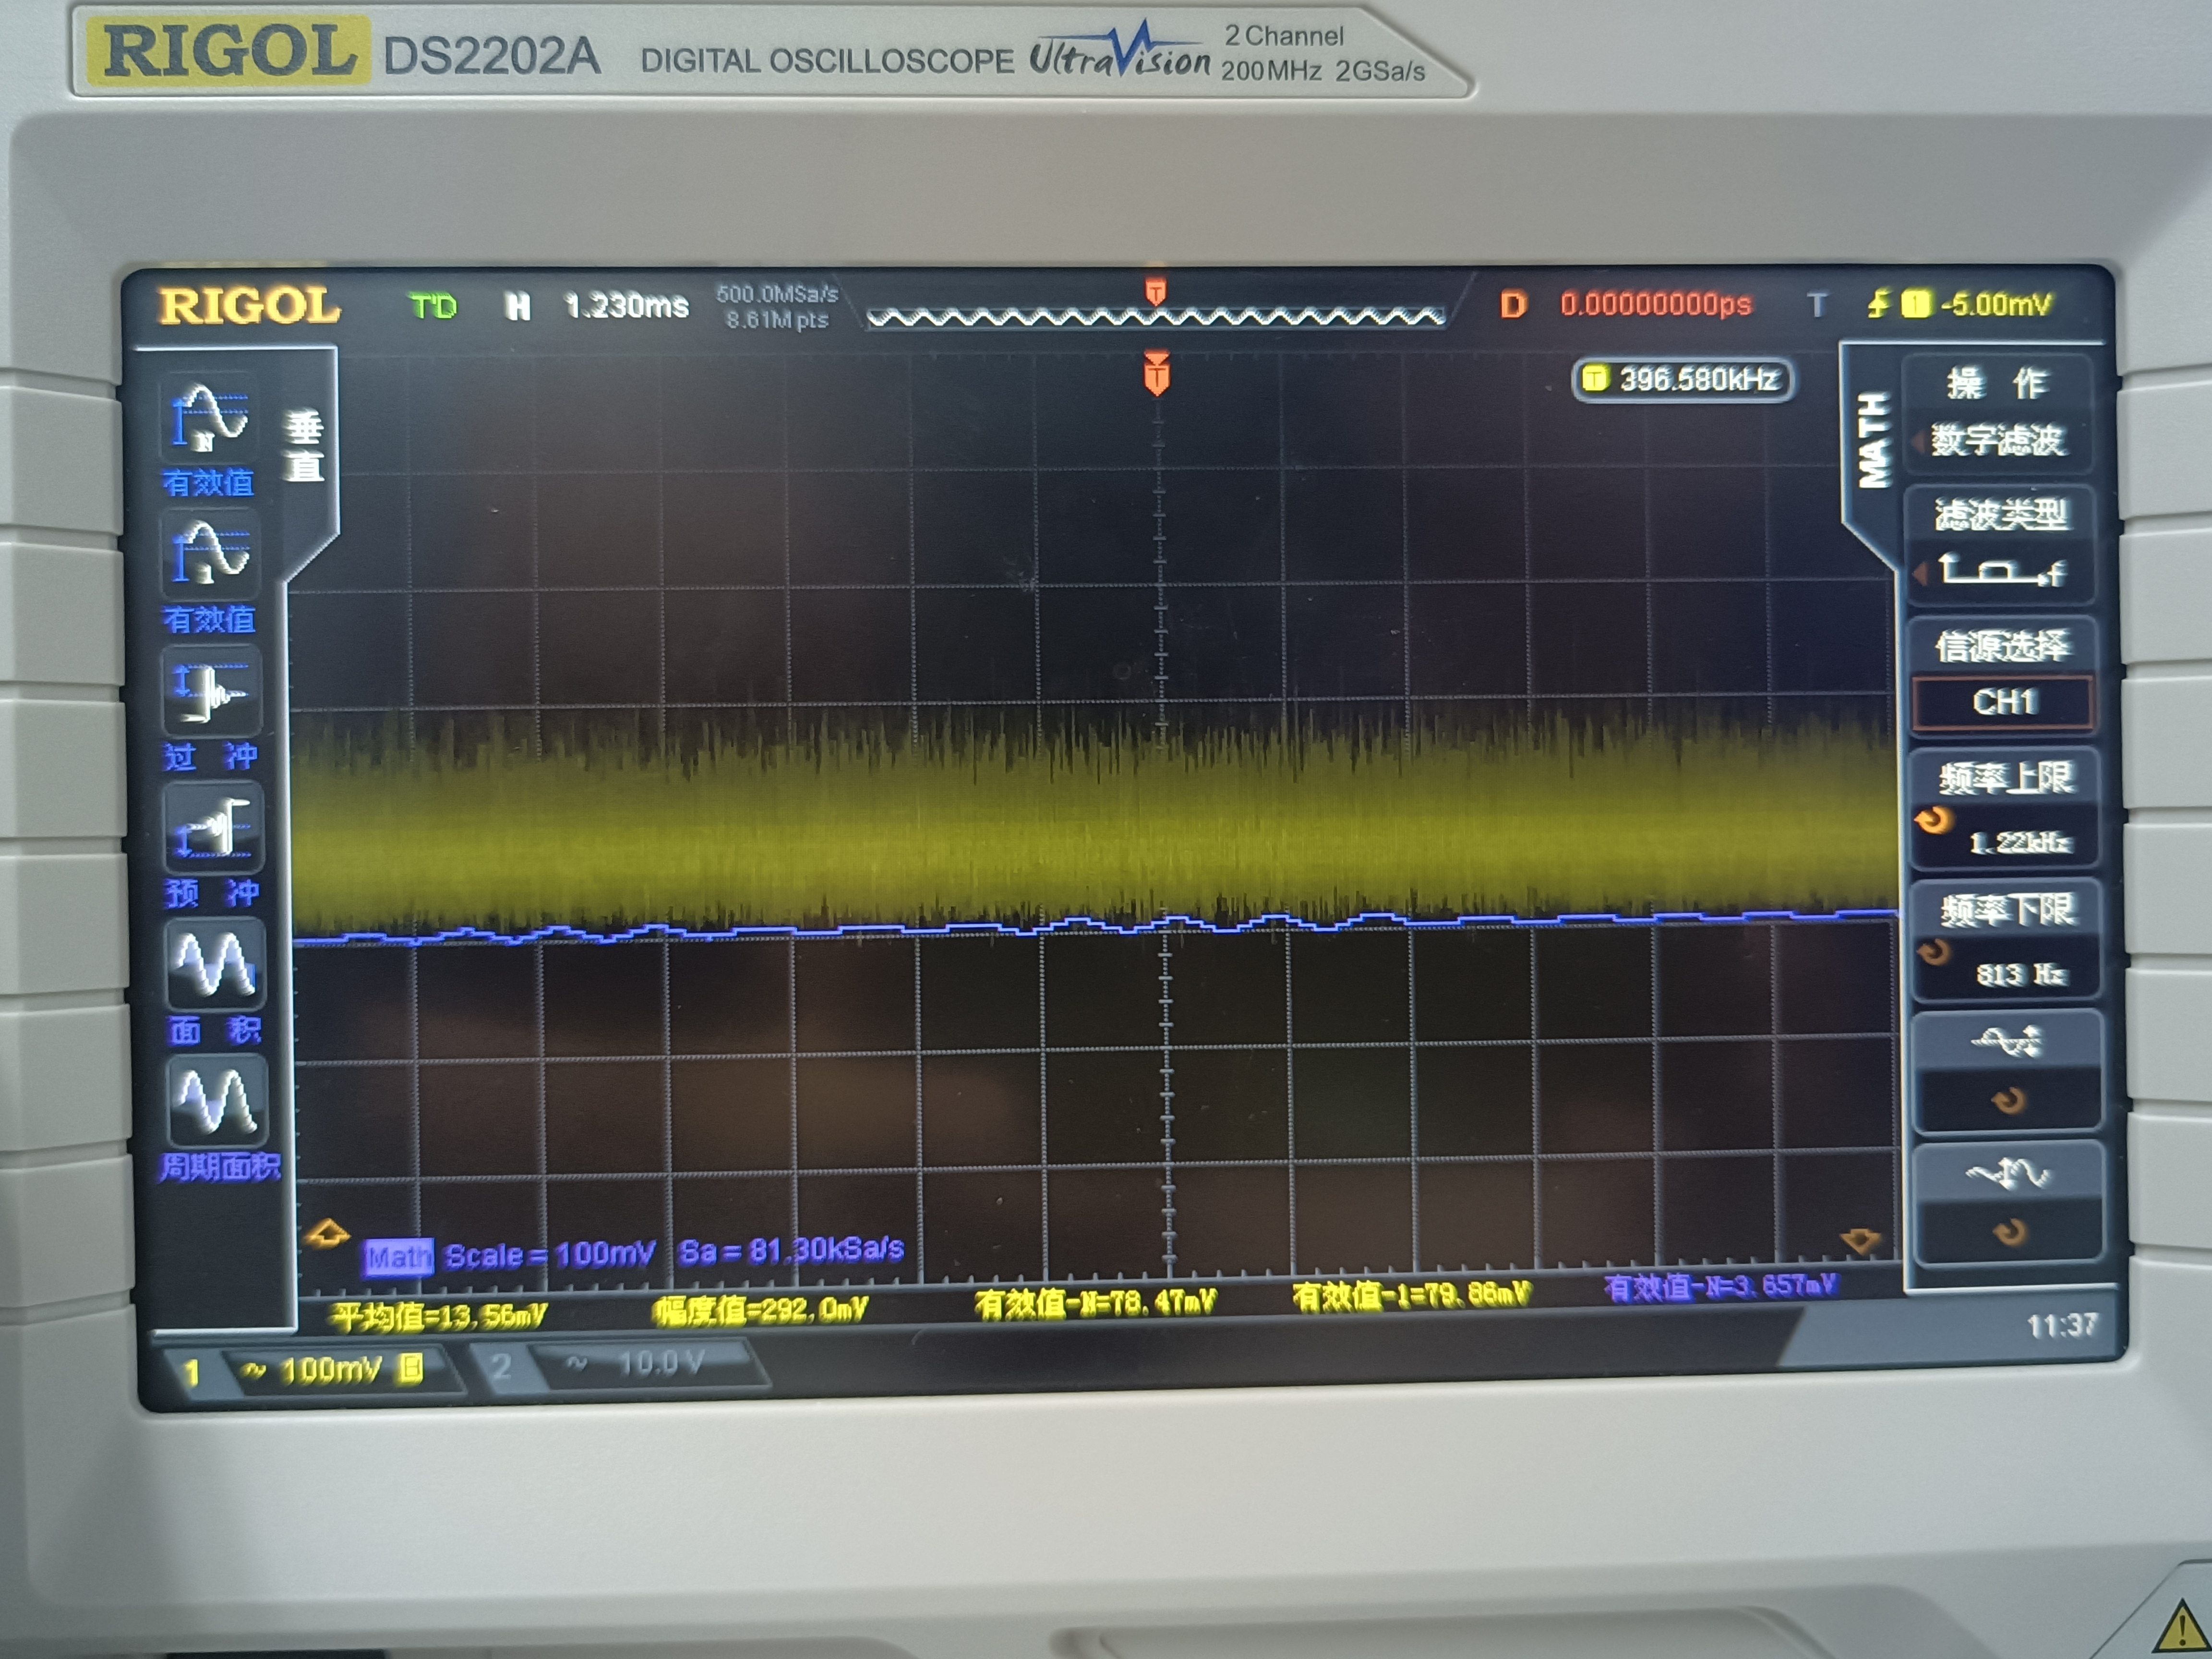
\includegraphics[width=0.32\linewidth]{6.2.jpg}}
		\quad
		\subfloat[-80dB]{\label{6.3}
		\includegraphics[width=0.32\linewidth]{6.3.jpg}}
		\quad
		\caption{强噪声背景检查弱信号}
		\label{强噪声背景检查弱信号}
		\end{figure}



	
	% 问题记录
	\subsection{实验过程遇到问题及解决办法}
	\begin{enumerate}
		\item 实验总体较为繁琐,但是在仔细阅读实验指引和求助老师后,最终按时完成了实验。
		\item 实验中的一些操作较为基础,目的是逐步熟悉仪器,但是在实验过程中出现了由于实验指引稍显简略从而导致不得不不断询问老师来推进实验。
		\item 实验中关于示波器和锁相放大器的调节较为繁琐,并且在调节时发现其中一段连接线较为松动,从而导致了输出的信号非常波动,更换线路后减轻了这个问题。
	\end{enumerate}
	% ---
	
	
	
	% 分析与讨论	
	\clearpage
	
	% 顶栏
	\begin{table}
		\renewcommand\arraystretch{1.7}
		\begin{tabularx}{\textwidth}{|X|X|X|X|}
			\hline
			专业:& 物理学 &年级:& 2022级\\
			\hline
			姓名: & 黄罗琳 & 学号:& 22344001\\
			\hline
			日期:& 2024/9/20& 评分: &\\
			\hline
		\end{tabularx}
	\end{table}
	% ---
	
	% 小标题
	\section{D1 锁相放大器与弱信号测量(1)\quad\heiti 分析与讨论}
	% ---
	
	% 数据处理
	\subsection{实验数据分析}
	本实验中需要讨论的实验数据较少,很多实验相关的原理问题已经在前一部分关于实验过程与结果的叙述中完成,完整性较好,故这里不再进行完整的实验分析。

	需要注意的是,本小组在第一次实验中便已经完成对于1.6部分的测量,并给出了一些分析,并且实验中的结果也同样验证了在1.8中结合表格对锁相放大器带宽的计算。

	此外,实验1.8中,可以明显看出锁相放大器的优势,超级高的信噪比体现了其在滤波作用时的极佳的实验效果。

	
	
	% ---
	
	% 实验后思考题
	\subsection{实验后思考题}
	
	%思考题1
	\begin{question}
		描述用教学实验箱配制不同信噪比信号的原理;实验箱生成的噪声是否为白噪声?
		\end{question}
		教学实验箱通过内置的100mVrms白噪声发生器来生成噪声,该发生器利用双极性晶体管的散粒噪声特性,从而产生高质量的白噪声。使用拨码器可以选择不同的输出电压,如100mVrms、10mVrms和1.0mVrms,分别对应0dB、20dB和40dB的信号衰减。结合锁相放大器OE1022的正弦波输出和外部信号衰减器,可以生成从100nVrms到5Vrms的正弦信号。通过调整有效信号和噪声的强度,可以灵活配置不同信噪比的信号。
		
		实验箱所生成的噪声确实是白噪声,因为其功率谱密度在广泛频率范围内均匀分布,示波器频域分析结果显示没有显著的峰值,符合白噪声特征。
	% 思考题2
	\begin{question}
		随着信噪比的改变,信号 $R$ 和相位差 $\theta$ 的测量值会有什么影响?
	\end{question}
	实验中发现,随着信噪比的减小,相位差 θ 的测量值抖动会变大,而信号 R 的测量误差也可能会增大。这是因为较低的信噪比导致信号中噪声成分的相对增加,从而影响测量的准确性。
	% 思考题3
	\begin{question}
		所有的噪声都可以用锁相放大器消除吗?锁相放大器的理论检测极限是多少?受什么
限制?(提示:降低信噪比后,锁相放大器的测量值偏差变大的原因是什么?缩小 LPF 带宽能缩小该
偏差吗?为什么?)
	\end{question}
	不是,锁相放大器无法消除所有噪声,同频噪声就属于此类。此外,缩小滤波器带宽虽然可以减少噪声,但代价是增加时间常数,从而抹平输入信号随时间的变化,可能导致有用信息的丢失。锁相放大器的理论检测极限由动态储备决定,动态储备由过载电平(OVL)与满刻度输出时的输入电平(FS)决定。OVL与信噪比相关,FS则受系统增益限制。当信号强度降低、信噪比减小时,最大噪声容量下降,动态储备减少,这会导致系统的热噪声使测量值的偏差增大。
	% ---
	
	\begin{question}
		请比较锁相放大器与示波器(经过带通滤波后)测量不同信噪比信号的结果,分析两种测量仪器(方法)的优势与劣势。
		\end{question}
		
		1. 锁相放大器

		   (a) 优势:在低信噪比条件下,示波器可能无法准确测量有效值 \( R \),而锁相放大器仍能保持良好的工作性能。此外,锁相放大器能够测量相位差等多种物理量,适用范围更广。

		   (b) 劣势:锁相放大器的显示信号信息相对有限,不能提供直观的波形展示,可能需要额外的解释或数据处理来理解测量结果。
		
		2. 示波器

		   (a) 优势:示波器提供较高的灵活度,可以实时观察信号的时域和频域图形,直观性较强,便于快速理解信号特性。

		   (b) 劣势:在低信噪比情况下,示波器无法有效测量信号的有效值,导致在噪声环境下的测量精度较低。
		
		极限比较:为了提高测量值的信噪比,锁相放大器可以选择窄带宽的低通滤波器(LPF),从而降低背景噪声。此外,通过对 \( X \) 值和 \( Y \) 值进行多次采样后求平均(,也可以进一步提高信噪比。这些方法使得锁相放大器在处理低信噪比信号时具有明显优势,而示波器在实时观测和直观性上占有优势,但在低信噪比情况下的测量能力受限。
	% 结语部分
	\clearpage
	
	% 小标题
	\section{D1 锁相放大器与弱信号测量(1) \quad\heiti 结语}
	% ---
	
	% 总结、杂谈与致谢
	\subsection{实验心得和体会、意见建议等}
	\begin{enumerate}
		\item 实验所需要的时间的确较长,由于对实验仪器的不熟悉,会导致前期工作大大延长,并且由于在实验开始时对于锁相放大器能够达到的实验效果和结果没有一个合理预期,从而导致了实验过程中存在一步一个坎的情况。
		\item 实验最终带来的震撼,明显的信噪比的差距,可以明显体现出锁相放大器的优势,很期待下一次的实验。
		\item 感谢\textbf{何老师和柳老师}在实验中详细为我解答每一个问题,让我能够按时完成实验,感谢您!
		\item 相关源文件(Latex)已上传Github,相关库包含实验报告内容,如需要查看可联系我进行查阅。
	\end{enumerate}
	\quad \large \textbf{感谢您对于此篇实验报告的阅读与批改,祝您工作顺利!}
	

	% 附件
	\subsection{附件及实验相关的软硬件资料等}
	\begin{figure}[{H}]
		\centering
		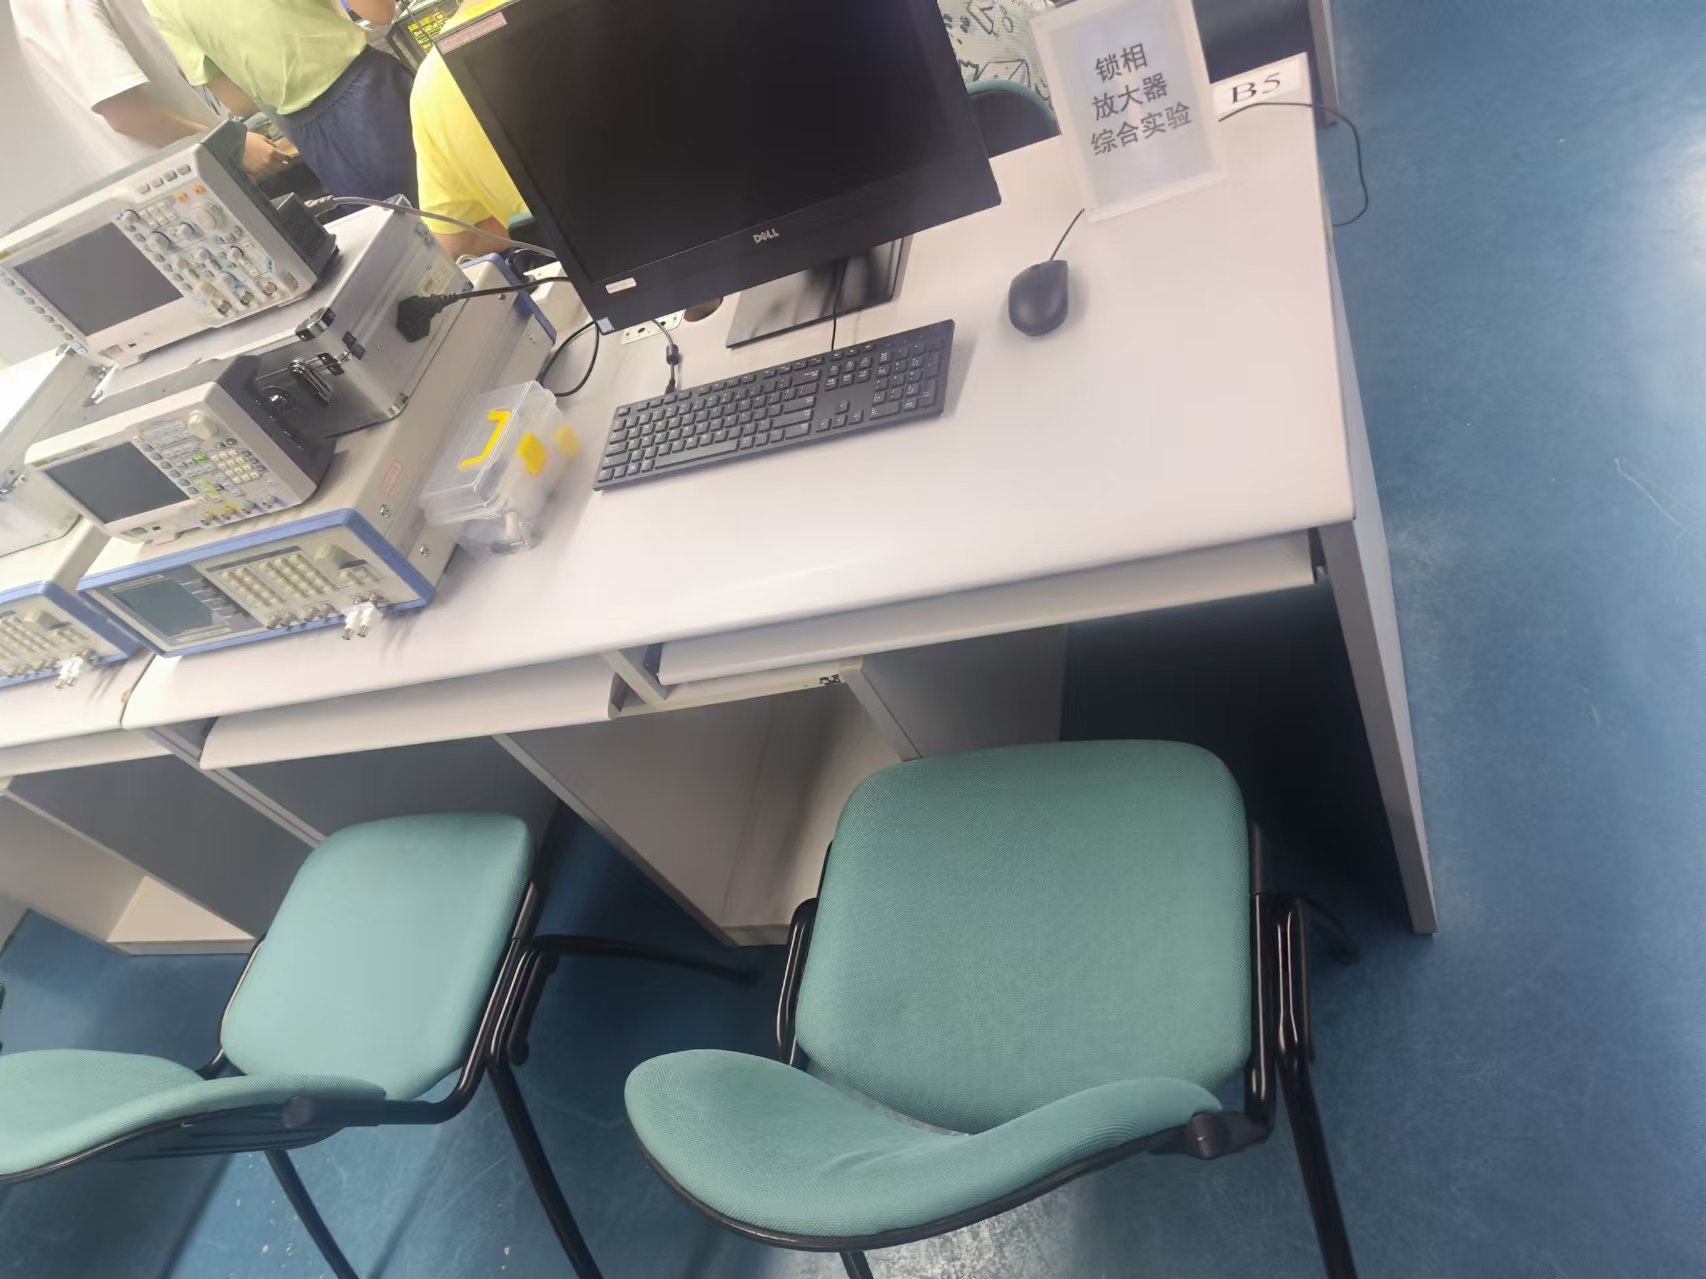
\includegraphics[width=0.4\linewidth]{桌面.jpg}
		\caption{实验桌面整理}
		\label{}
	\end{figure}
	

	\begin{figure}[{H}]
		\centering
		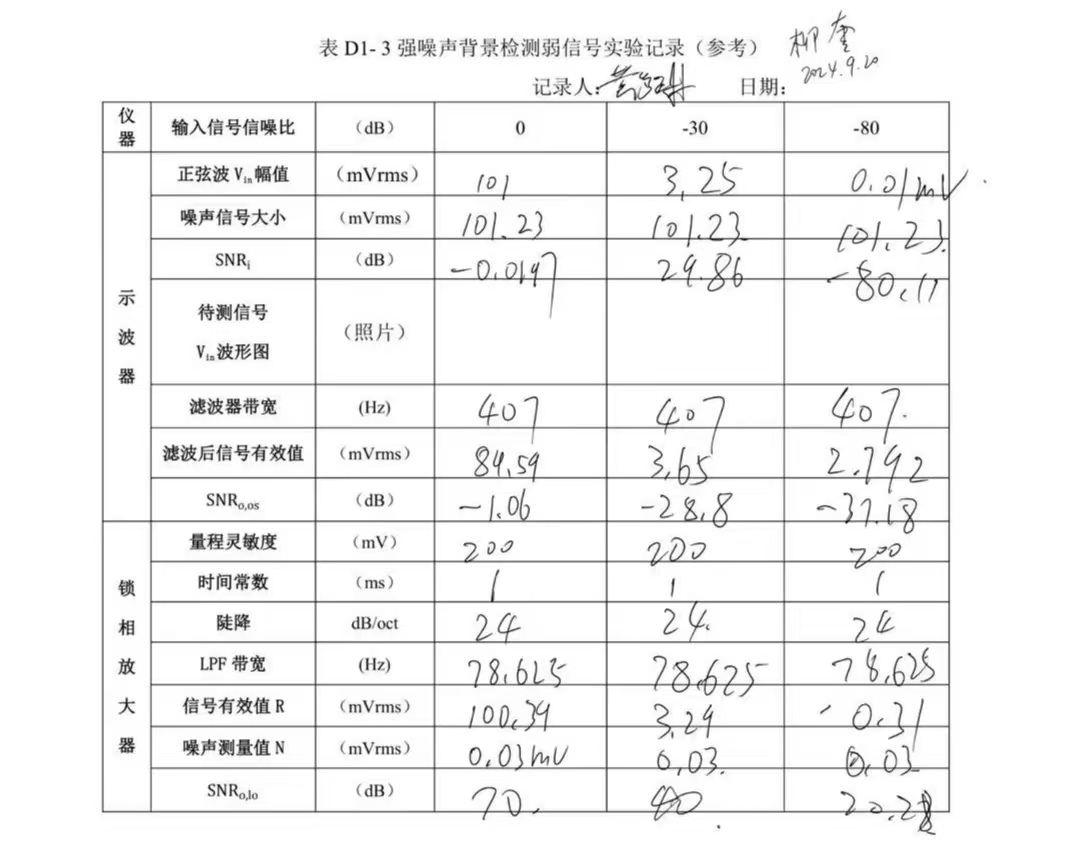
\includegraphics[width=0.4\linewidth]{原始.jpg}
		\caption{实验原始数据及签字}
		\label{}
	\end{figure}

	% ---
	
	
\end{document}